%% USPSC-modelo-ICMCp.tex
% ---------------------------------------------------------------
% USPSC: Modelo de Trabalho Acadêmico (tese de doutorado, dissertacao de
% mestrado e trabalhos monograficos em geral) em conformidade com 
% ABNT NBR 14724:2011: Informação e documentação - Trabalhos acadêmicos -
% Apresentação
%----------------------------------------------------------------
%% Esta é uma customização do abntex2-modelo-trabalho-academico.tex de v-1.9.5 laurocesar 
%% para as Unidades do Campus USP de São Carlos:
%% EESC - Escola de Engenharia de São Carlos
%% IAU - Instituto de Arquitetura e Urbanismo
%% ICMC - Instituto de Ciências Matemáticas e de Computação
%% IFSC - Instituto de Física de São Carlos
%% IQSC - Instituto de Química de São Carlos
%%
%% Este trabalho utiliza a classe USPSC (USPSC.cls e USPSC1.cls) que é mantida 
%% pela seguinte equipe:
%% 
%% Coordenação e Programação:
%%   - Marilza Aparecida Rodrigues Tognetti - marilza@sc.usp.br (PUSP-SC)
%%   - Ana Paula Aparecida Calabrez - aninha@sc.usp.br (PUSP-SC)
%% Normalização:
%%   - Brianda de Oliveira Ordonho Sigolo - brianda@usp.br (IAU)
%%   - Eduardo Graziosi Silva - edu.gs@sc.usp.br (EESC)
%%   - Eliana de Cássia Aquareli Cordeiro - eliana@iqsc.usp.br (IQSC)
%%   - Flávia Helena Cassin - cassinp@sc.usp.br (EESC)
%%   - Maria Cristina Cavarette Dziabas - mcdziaba@ifsc.usp.br (IFSC)
%%   - Regina Célia Vidal Medeiros - rcvmat@icmc.usp.br (ICMC)
%%
%% Os modelos desenvolvidos utilizam diversos arquivos relacionado em 
%% 2.1 Pacote USPSC: Classe USPSC e modelos de trabalhos acadêmicos	do Tutorial do Pacote 
%%  USPSC para modelos de trabalhos de acadêmicos em LaTeX - versão 3.2

%----------------------------------------------------------------
%% Sobre a classe abntex2.cls:
%% abntex2.cls, v-1.9.5 laurocesar
%% Copyright 2012-2015 by abnTeX2 group at https://www.abntex.net.br/ 
%%
%----------------------------------------------------------------

\documentclass[
% -- opções da classe memoir --
12pt,		% tamanho da fonte
openright,	% capítulos começam em pág ímpar (insere página vazia caso preciso)
%twoside, % para impressão em anverso (frente) e verso. Oposto a oneside - Nota: utilizar \imprimirfolhaderosto*
oneside,  % para impressão em páginas separadas (somente anverso) -  Nota: utilizar \imprimirfolhaderosto
% ATENCAO: com twoside as margens sao ESPELHADAS. \setlrmarginsandblock{3cm}{2cm}
% passa a significar 3cm na borda INTERNA, entao as paginas PARES ficam com 2cm a
% esquerda e 3cm a direita, deslocamento de 1cm (28pt) entre pagina par e impar.
% Com oneside todas as paginas ficam 3cm a esquerda e 2cm a direita.
% inclua uma % antes do comando twoside e exclua a % antes do oneside 
a4paper,			% tamanho do papel. 
% -- opções da classe abntex2 --
chapter=TITLE,		% títulos de capítulos convertidos em letras maiúsculas
% -- opções do pacote babel --
english,			% idioma adicional para hifenização
french,				% idioma adicional para hifenização
spanish,			% idioma adicional para hifenização
brazil				% o último idioma é o principal do documento
% {USPSC-classe/USPSC} configura o cabeçalho contendo apenas o número da página
]{USPSC-classe/USPSC}
%]{USPSC-classe/USPSC1}
% Inclua % antes de ]{USPSC-classe/USPSC} e retire a % antes de %]{USPSC-classe/USPSC1} para utilizar o 
% cabeçalho diferenciado para as páginas pares e ímpares:
%- páginas ímpares: com seções ou subseções e o número da página
%- páginas pares: com o número da página e o título do capítulo 
% ---
% ---
% Pacotes básicos - Fundamentais 
% ---
\usepackage[T1]{fontenc}		% Seleção de códigos de fonte.
\usepackage[utf8]{inputenc}		% Codificação do documento (conversão automática dos acentos)
\usepackage{lmodern}			% Usa a fonte Latin Modern
% Para utilizar a fonte Times New Roman, inclua uma % no início do comando acima  "\usepackage{lmodern}"
% Abaixo, tire a % antes do comando  \usepackage{times}
%\usepackage{times}		    	% Usa a fonte Times New Roman	
% Para usar a fonte , lembre-se de tirar a % do comando %\renewcommand{\ABNTEXchapterfont}{\rmfamily}, localizado mais abaixo, logo após "Outras opções para nota de rodapé no Sistema Numérico" 				
\usepackage{lastpage}			% Usado pela Ficha catalográfica
\usepackage{indentfirst}		% Indenta o primeiro parágrafo de cada seção.
\usepackage{color}				% Controle das cores
\usepackage{graphicx}			% Inclusão de gráficos
\usepackage{float} 				% Fixa tabelas e figuras no local exato
\usepackage{placeins}           % \FloatBarrier: impede float de atravessar secao
\usepackage{etoolbox}           % usado para zerar cola vertical dentro dos floats
\usepackage{chemfig}            % Para escrever reações químicas
\usepackage{chemmacros}         % Para escrever reações químicas
\usepackage{tikz}				% Para escrever reações químicas e outros
\usetikzlibrary{positioning}
\usepackage{microtype} 			% para melhorias de justificação
\usepackage{pdfpages}
\usepackage{makeidx}            % para gerar índice remissivo
\usepackage{hyphenat}          % Pacote para retirar a hifenizacao DO TEXTO
\usepackage[absolute]{textpos} % Pacote permite o posicionamento do texto
\usepackage{eso-pic}           % Pacote para incluir imagem de fundo
\usepackage{makebox}           % Pacote para criar caixa de texto
% ---

% ---
% Pacotes de citações
% Citações padrão ABNT
% ---
% Sistemas de chamada: autor-data ou numérico.
% Sistema autor-data
% ATENCAO: abnt-cite-style=AUTHORYEAR reproduz o padrao do texto original,
% com o sobrenome em CAIXA ALTA nas citacoes entre parenteses (NBR 10520:2002).
% O padrao do template USPSC e AuthorYEAR, conforme a NBR 10520:2023.
% Para voltar ao padrao do template, troque o valor abaixo ou remova a opcao.
\usepackage[alf, abnt-cite-style=AUTHORYEAR, abnt-emphasize=bf, abnt-thesis-year=both, abnt-repeated-author-omit=no, abnt-last-names=abnt, abnt-etal-cite=3, abnt-etal-list=3, abnt-etal-text=it, abnt-and-type=e, abnt-doi=doi, abnt-url-package=none, abnt-verbatim-entry=no]{abntex2cite}
\bibliographystyle{USPSC-classe/abntex2-alf-USPSC}
% Se o idioma for o inglês, inclua % no comando acima e exclua o % do comando abaixo
%\bibliographystyle{USPSC-classe/abntex2-alfeng-USPSC}

% Para o IQSC, que indica todos os autores nas referências, incluir % no início dos comandos acima e retirar a % dos comandos abaixo 
%\usepackage[alf, abnt-emphasize=bf, abnt-thesis-year=both, abnt-repeated-author-omit=no, abnt-last-names=abnt, abnt-etal-cite=3, abnt-etal-list=0, abnt-etal-text=it, abnt-and-type=e, abnt-doi=doi, abnt-url-package=none, abnt-verbatim-entry=no]{abntex2cite} 
%\bibliographystyle{USPSC-classe/abntex2-alf-USPSC}
% Se o idioma for o inglês, exclua % no comando acima ou do comando abaixo
%\bibliographystyle{USPSC-classe/abntex2-alfeng-USPSC}

% Sistema Numérico
% Para citações numéricas, sistema adotado pelo IFSC, incluir % no início dos comandos acima e retirar a % dos comandos abaixo
%\usepackage{cite}              % agrupa citações numéricas consecutivas 
%\usepackage[num, abnt-emphasize=bf, abnt-thesis-year=both, abnt-repeated-author-omit=no, abnt-last-names=abnt, abnt-etal-cite=3, abnt-etal-list=3, abnt-etal-text=it, abnt-and-type=e, abnt-doi=doi, abnt-url-package=none, abnt-verbatim-entry=no]{abntex2cite} 
%\bibliographystyle{USPSC-classe/abntex2-num-USPSC}
% Se o idioma for o inglês, exclua % no comando acima ou do comando abaixo
%\bibliographystyle{USPSC-classe/abntex2-numeng-USPSC}

% Complementarmente, verifique as instruções abaixo sobre os Pacotes de Nota de rodapé
% ---
% Pacotes de Nota de rodapé
% Configurações de nota de rodapé

% O presente modelo adota o formato numérico para as notas de rodapés quando utiliza o sistema de chamada autor-data para citações e referências. Para utilizar o sistema de chamada numérico para citações e referências, habilitar um dos comandos abaixo.
% Há diversa opções para nota de rodapé no Sistema Numérico.  Para o IFSC, habilitade o comando abaixo.

%\renewcommand{\thefootnote}{\fnsymbol{footnote}}  %Comando para inserção de símbolos em nota de rodapé

% Outras opções para nota de rodapé no Sistema Numérico:
%\renewcommand{\thefootnote}{\alph{footnote}}      %Comando para inserção de letras minúscula em nota de rodapé
%\renewcommand{\thefootnote}{\Alph{footnote}}      %Comando para inserção de letras maiúscula em nota de rodapé
%\renewcommand{\thefootnote}{\roman{footnote}}     %Comando para inserção de números romanos minúsculos  em nota de rodapé
%\renewcommand{\thefootnote}{\Roman{footnote}}     %Comando para inserção de números romanos minúsculos  em nota de rodapé

\renewcommand{\footnotesize}{\small} %Comando para diminuir a fonte das notas de rodapé
%Para utilizar a fonte Times New Roman, inclua retire % do início do comando abaixo 
%\renewcommand{\ABNTEXchapterfont}{\rmfamily}

% ---
% Pacote para agrupar a citação numérica consecutiva
% Quando for adotado o Sistema Numérico, a exemplo do IFSC, habilite 
% o pacote cite abaixo retirando a porcentagem antes do comando abaixo
%\usepackage[superscript]{cite}	

% ---
% Pacotes adicionais, usados apenas no âmbito do Modelo Canônico do abnteX2
% ---
% \usepackage{lipsum}			% para geração de dummy text (não utilizado neste trabalho)
% ---
% Pacotes adicionais deste trabalho
\usepackage{amsmath}            % fórmulas (valores SHAP, limiares)
\usepackage{amssymb}            % símbolos matemáticos (\mathbb)
% Macro para o rótulo |SHAP| usado em legendas e no texto
\newcommand{\shapabs}{\ensuremath{|\mathrm{SHAP}|}}
% Legendas numeradas fora de ambiente flutuante, para quadros/tabelas longos
% construidos com longtable (recurso nativo da classe memoir).
\newfixedcaption{\quadrocaption}{quadro}
\newfixedcaption{\tabelacaption}{table}
% ---

% pacotes de tabelas
\usepackage{multicol}	% Suporte a mesclagens em colunas
\usepackage{multirow}	% Suporte a mesclagens em linhas
\usepackage{longtable}	% Tabelas com várias páginas
\usepackage{threeparttablex}    % notas no longtable
\usepackage{array}

% ----
% Compatibilização com a ABNT NBR 6023:2018 e 10520:2023
% Para tirar <> da URL e tornar as expressões latinas em itálico
\usepackage{USPSC-classe/ABNT6023-10520}
% As demais compatibilizações estão nos arquivos abntex2-alf-USPSC.bst,abntex2-alfeng-USPSC.bst, abntex2-num-USPSC.bst e abntex2-numeng-USPSC.bst, dependendo do idioma do textos e se o sistemas de chamada for autor-data ou numérico, conforme explicitado acima.
% ----

\newcommand{\checkbox}{\tikz[baseline=-0.55ex]\draw[line width=0.35pt] (0,0) rectangle (0.20,0.20);}
\newcommand{\formline}[1]{\rule{#1}{0.35pt}}
\newcommand{\choice}[1]{\noindent\checkbox\hspace{0.12cm}#1\par}

% ---
% DADOS INICIAIS - Define sigla com título, área de concentração e opção do Programa 
% ConsulteDCCp a tabela referente aos Programas, áreas e opções de sua unidade contante do
% arquivo USPSC-Siglas estabelecidas para os Programas de Pós-Graduação nos APÊNDICES B-J
\siglaunidade{ICMC}
\programa{MBAIAp}
% Os demais dados deverão ser fornecidos no arquivo USPSC-pre-textual-UUUU ou USPSC-TCC-pre-textual-UUUU, onde UUUU é a sigla da Unidade. 
% Exemplo:USPSC-pre-textual-IFSC.tex
% ---
% Configurações de aparência do PDF final
% alterando o aspecto da cor azul
\definecolor{blue}{RGB}{41,5,195}

% informações do PDF
\makeatletter
\hypersetup{
	%pagebackref=true,
	pdftitle={\@title}, 
	pdfauthor={\@author},
	pdfsubject={\imprimirpreambulo},
	pdfcreator={LaTeX with abnTeX2},
	pdfkeywords={abnt}{latex}{abntex}{USPSC}{trabalho acadêmico}, 
	colorlinks=true,       		% false: boxed links; true: colored links
	linkcolor=black,          	% color of internal links
	citecolor=black,        		% color of links to bibliography
	filecolor=black,      		% color of file links
	urlcolor=black,
	%Para habilitar as cores dos links, retire a % antes dos comandos abaixo e inclua a % antes das 4 linhas de comando acima 
	%linkcolor=blue,            	% color of internal links
	%citecolor=blue,        		% color of links to bibliography
	%filecolor=magenta,      		% color of file links
	%urlcolor=blue,
	bookmarksdepth=4	
}
\makeatother
% --- 
% --- 
% Espaçamentos entre linhas e parágrafos 
% --- 

% O tamanho do parágrafo é dado por:
\setlength{\parindent}{1.3cm}

% Controle do espaçamento entre um parágrafo e outro:
\setlength{\parskip}{0.2cm plus 2pt minus 1pt}
% A elasticidade (plus/minus) e necessaria: o memoir aplica \flushbottom, que estica
% cola vertical ate a pagina fechar no rodape. Com \parskip rigido nao ha cola nos
% paragrafos, e o estiramento vai todo para os espacos de titulo e de float, o que
% faz o espacamento variar de pagina para pagina.

% \raggedbottom: a pagina termina onde o texto termina, sem esticar nada. E o que
% garante espacamento identico entre paragrafos em todas as paginas. Para voltar ao
% comportamento anterior (rodape alinhado, espacamento variavel), troque por \flushbottom.
\raggedbottom

% Espaco antes de cada entrada de capitulo no Sumario (a classe usa 1em).
% Reduzido para o Sumario caber em uma pagina.
\setlength{\cftbeforechapterskip}{0.5em}

% Dentro de figure/table/quadro os ambientes center e flushleft do bloco de Fonte
% acrescentam \topsep acima e abaixo (cerca de 40pt por float). Zerar aqui uniformiza
% o espacamento de todos os floats sem precisar reescrever os blocos um a um.
\newcommand{\USPSCfloatglue}{%
  \setlength{\topsep}{0pt}\setlength{\partopsep}{0pt}%
  \setlength{\parskip}{0pt}}
\AtBeginEnvironment{figure}{\USPSCfloatglue}
\AtBeginEnvironment{table}{\USPSCfloatglue}
\AtBeginEnvironment{quadro}{\USPSCfloatglue}

% ---
% compila o sumário e índice
\makeindex
% ---
% ----
% Início do documento
% ----
\begin{document}

% Seleciona o idioma do documento (conforme pacotes do babel)
\selectlanguage{brazil}
% Se o idioma do texto for inglês, inclua uma % antes do 
%      comando \selectlanguage{brazil} e 
%      retire a % antes do comando abaixo
%\selectlanguage{english}

% Retira espaço extra obsoleto entre as frases.
\frenchspacing 

% --- Formatação dos Títulos
\renewcommand{\ABNTEXchapterfontsize}{\fontsize{12}{12}\bfseries}
\renewcommand{\ABNTEXsectionfontsize}{\fontsize{12}{12}\bfseries}
\renewcommand{\ABNTEXsubsectionfontsize}{\fontsize{12}{12}\normalfont}
\renewcommand{\ABNTEXsubsubsectionfontsize}{\fontsize{12}{12}\normalfont}
\renewcommand{\ABNTEXsubsubsubsectionfontsize}{\fontsize{12}{12}\normalfont}


% ----------------------------------------------------------
% ELEMENTOS PRÉ-TEXTUAIS
% ----------------------------------------------------------
% ---
% Capa
% ---
%imprimircapa
% 26/03/2021 ----------------
%Capa do ICMC
%% USPSC-CapaICMC.tex
\AddToShipoutPicture{\BackgroundPic}
%-------------
\begin{minipage}[c]{144mm}
   \centering
   \begin{textblock*}{144mm}(61mm,65mm)
   \vspace*{1,2cm}
   \linespread{0.5}
   \ABNTEXchapterfont\bfseries\Large
   \textcolor{capa-azul}{\nohyphens{\imprimirtitulo}}
   \end{textblock*}
\end{minipage}
\vfill
\vspace*{5cm}
\begin{minipage}[t][65mm][t]{125mm}
   \begin{textblock*}{130mm}(81mm,123mm)
      \ABNTEXchapterfont\bfseries\Large
      \textcolor{capa-azul}{\nohyphens{\imprimirautor}} 
      \vfill
      \vspace{9pt}
      \ABNTEXsubsectionfontsize\small
      \renewcommand{\ABNTEXsubsectionfontsize}{\fontsize{10}{6}\normalfont}
      \ABNTEXsubsectionfontsize 
      \textcolor{capa-azul}{\nohyphens{\imprimirnotacapaicmc}}
      \renewcommand{\ABNTEXsubsectionfontsize}{\fontsize{12}{12}\normalfont}
   \end{textblock*}	
\end{minipage} 
% ---

\AddToShipoutPicture{\BackgroundBranco}

\includepdf{USPSC-TA-PreTextual/USPSC-PaginaEmBranco.pdf}
% ----------------
% ---
% Folha de rosto do ICMC
% (o * indica impressão em anverso (frente) e verso )
% ---
\imprimirfolharostocar
%\imprimirfolharostocar*

% Folha de rosto padrão do Pacote USPSC
% (o * indica impressão em anverso (frente) e verso )
% ---
%\imprimirfolhaderosto
%\imprimirfolhaderosto*
% ---
% ---
% Inserir a ficha catalográfica em pdf
% ---
% A biblioteca da sua Unidade lhe fornecerá um PDF com a ficha
% catalográfica definitiva. 
% Quando estiver com o documento, salve-o como PDF no diretório
% do seu projeto como fichacatalografica.pdf e inclua o arquivo
% utilizando o comando abaixo:

%\includepdf{USPSC-TA-PreTextual/USPSC-fichacatalografica.pdf}

% Se você optar por elaborar a ficha catalográfica, deverá 
% incluir uma % antes da linha % antes
% do comando %% USPSC-fichacatalografica.tex
% ---
% Inserir a ficha bibliografica
% ---
% Isto é um exemplo de Ficha Catalográfica, ou ``Dados internacionais de
% catalogação-na-publicação''. Você pode utilizar este modelo como referência. 
% Porém, provavelmente a biblioteca da sua universidade lhe fornecerá um PDF
% com a ficha catalográfica definitiva após a defesa do trabalho. Quando estiver
% com o documento, salve-o como PDF no diretório do seu projeto e substitua todo
% o conteúdo de implementação deste arquivo pelo comando abaixo:
%
\begin{fichacatalografica}
	\hspace{-1.4cm}
	\imprimirnotaautorizacao \\ \\
	%\sffamily
	\vspace*{\fill}					% Posição vertical
\begin{center}					% Minipage Centralizado
  \imprimirnotabib \\
  \begin{table}[htb]
	\scriptsize
	\centering	
	\begin{tabular}{|p{0.9cm} p{8.7cm}|}
		\hline
	      & \\
		  &	  \imprimirautorficha     \\
		
		 \imprimircutter & 
							\hspace{0.4cm}\imprimirtitulo~  / ~\imprimirautor~ ;  ~\imprimirorientadorcorpoficha. -- 	\imprimirlocal, \imprimirdata.   \\
		
		  &  % Para incluir nota referente à versão corrigida no corpo da ficha,
			  % incluir % no início da linha acima e tirar a % do início da linha abaixo
			  %	\hspace{0.4cm} \imprimirtitulo~  / ~\imprimirautor~ ; ~\imprimirorientadorcorpoficha~- ~\imprimirnotafolharosto. -- \imprimirlocal, \imprimirdata.  \\
		
			\hspace{0.4cm}\pageref{LastPage} p. : il. (algumas color.) ; 30 cm.\\ 
		  & \\
		  & 
		    \hspace{0.4cm}\imprimirnotaficha ~--~ 
						  \imprimirunidademin, 
						  \imprimiruniversidademin, 
		                  \imprimirdata. \\ 
		  & \\                 
		   % Para incluir nota referente à versão corrigida em notas,
		    % incluir uma % no início da linha acima e	
		    % tirar a % do início da linha abaixo
		    % & \hspace{0.4cm}\imprimirnotafolharosto \\ 
		  & \\ 
		  & \hspace{0.4cm}1. Churn. 2. Machine Learning. 3. Random Forest. 4. RFM. 5. E-commerce. I. \imprimirorientadorficha. 
		   II. Título. \\
	
		     %Se houver co-orientador, inclua % antes da linha (antes de II. Título.) 
		     %          e tire a % antes do comando abaixo 
		     %III. Título. \\   
		  \hline
	\end{tabular}
  \end{table}
\end{center}
\end{fichacatalografica}
% ---

 
% e retirar o % do comando abaixo
%% USPSC-fichacatalografica.tex
% ---
% Inserir a ficha bibliografica
% ---
% Isto é um exemplo de Ficha Catalográfica, ou ``Dados internacionais de
% catalogação-na-publicação''. Você pode utilizar este modelo como referência. 
% Porém, provavelmente a biblioteca da sua universidade lhe fornecerá um PDF
% com a ficha catalográfica definitiva após a defesa do trabalho. Quando estiver
% com o documento, salve-o como PDF no diretório do seu projeto e substitua todo
% o conteúdo de implementação deste arquivo pelo comando abaixo:
%
\begin{fichacatalografica}
	\hspace{-1.4cm}
	\imprimirnotaautorizacao \\ \\
	%\sffamily
	\vspace*{\fill}					% Posição vertical
\begin{center}					% Minipage Centralizado
  \imprimirnotabib \\
  \begin{table}[htb]
	\scriptsize
	\centering	
	\begin{tabular}{|p{0.9cm} p{8.7cm}|}
		\hline
	      & \\
		  &	  \imprimirautorficha     \\
		
		 \imprimircutter & 
							\hspace{0.4cm}\imprimirtitulo~  / ~\imprimirautor~ ;  ~\imprimirorientadorcorpoficha. -- 	\imprimirlocal, \imprimirdata.   \\
		
		  &  % Para incluir nota referente à versão corrigida no corpo da ficha,
			  % incluir % no início da linha acima e tirar a % do início da linha abaixo
			  %	\hspace{0.4cm} \imprimirtitulo~  / ~\imprimirautor~ ; ~\imprimirorientadorcorpoficha~- ~\imprimirnotafolharosto. -- \imprimirlocal, \imprimirdata.  \\
		
			\hspace{0.4cm}\pageref{LastPage} p. : il. (algumas color.) ; 30 cm.\\ 
		  & \\
		  & 
		    \hspace{0.4cm}\imprimirnotaficha ~--~ 
						  \imprimirunidademin, 
						  \imprimiruniversidademin, 
		                  \imprimirdata. \\ 
		  & \\                 
		   % Para incluir nota referente à versão corrigida em notas,
		    % incluir uma % no início da linha acima e	
		    % tirar a % do início da linha abaixo
		    % & \hspace{0.4cm}\imprimirnotafolharosto \\ 
		  & \\ 
		  & \hspace{0.4cm}1. Churn. 2. Machine Learning. 3. Random Forest. 4. RFM. 5. E-commerce. I. \imprimirorientadorficha. 
		   II. Título. \\
	
		     %Se houver co-orientador, inclua % antes da linha (antes de II. Título.) 
		     %          e tire a % antes do comando abaixo 
		     %III. Título. \\   
		  \hline
	\end{tabular}
  \end{table}
\end{center}
\end{fichacatalografica}
% ---


% As informações que compõem a ficha catalográfica estão 
% definidas no arquivo USPSC-pre-textual-UUUU.tex
% ---f

% ---
% Folha de rosto adicional
% Para imprimir a folha de rosto adicional, exigida por algumas Unidades, a exemplo do ICMC,
% retire a % antes do comando abaixo

\imprimirfolhaderostoadic*

% ---
% ---
% Inserir errata
% ---

%%% USPSC-Errata.tex
\begin{errata}
	%\OnehalfSpacing 			
	A errata é um elemento opcional, que consiste de uma lista de erros da obra, precedidos pelas folhas e linhas onde eles ocorrem e seguidos pelas correções correspondentes. Deve ser inserida logo após a folha de rosto e conter a referência do trabalho para facilitar sua identificação, conforme a ABNT NBR 14724 \cite{nbr14724}.
	
	Modelo de Errata:
		
	\begin{flushleft} 
			\setlength{\absparsep}{0pt} % ajusta o espaçamento da referência	
			\SingleSpacing 
			\imprimirautorabr~ ~\textbf{\imprimirtituloresumo}.	\imprimirdata. \pageref{LastPage} p. 
			%Substitua p. por f. quando utilizar oneside em \documentclass
			%\pageref{LastPage} f.
			\imprimirtipotrabalho~-~\imprimirinstituicao, \imprimirlocal, \imprimirdata. 
 	\end{flushleft}
\vspace{\onelineskip}
\OnehalfSpacing 
\center
\textbf{ERRATA}
\vspace{\onelineskip}
\OnehalfSpacing 
\begin{table}[htb]
	\center
	\footnotesize
	\begin{tabular}{p{2cm} p{2cm} p{4cm} p{4cm} }
		\hline
		\textbf{Folha} & \textbf{Linha}  & \textbf{Onde se lê}  & \textbf{Leia-se}  \\
			\hline
			1 & 10 & auto-conclavo & autoconclavo\\
		\hline
	\end{tabular}
\end{table}
\end{errata}
% ---

% ---

% ---
% Inserir folha de aprovação
% ---

% A Folha de aprovação é um elemento obrigatório da NBR 4724/2011 (seção 4.2.1.3). 
% Após a defesa/aprovação do trabalho, gere o arquivo folhadeaprovacao.pdf da página assinada pela banca 
% e iclua o arquivo utilizando o comando abaixo:
%\includepdf{USPSC-TA-PreTextual/USPSC-folhadeaprovacao.pdf}
% Alternativa para a Folha de Aprovação:
% Se for a sua opção elaborar uma folha de aprovação, insira uma % antes do comando acima que inclui o arquivo folhadeaprovacao.pdf,
% tire o % do comando abaixo e altere o arquivo folhadeaprovacao.tex conforme suas necessidades
%\include{folhadeaprovacao}

\includepdf{USPSC-TA-PreTextual/USPSC-PaginaEmBranco.pdf}

% ---
% Dedicatória
% ---
%% USPSC-Dedicatoria.tex
\begin{dedicatoria}
   \vspace*{\fill}
   \centering
   \noindent
   \textit{À minha família, pelo apoio incondicional em cada etapa desta jornada.}
   \vspace*{\fill}
\end{dedicatoria}
% ---

% ---

% ---
% Agradecimentos
% ---
%% USPSC-Agradecimentos.tex
\begin{agradecimentos}
	À minha orientadora, Profa. Dra. Cibele M. Russo, pela orientação precisa, pela paciência e pelos ensinamentos fundamentais que guiaram a condução deste trabalho. Sua dedicação e suporte acadêmico foram essenciais para o sucesso desta jornada.

	Ao Instituto de Ciências Matemáticas e de Computação (ICMC/USP), pelo acolhimento e pela excelência do programa, que proporcionou a base necessária para o desenvolvimento desta pesquisa.

	À minha família, pelo apoio incondicional, compreensão e carinho durante todos os momentos de dedicação ao curso, sendo o meu porto seguro e a minha maior motivação para superar os desafios.

	Aos meus colegas de jornada no MBA em Inteligência Artificial e Big Data, pelas trocas de experiências e pelo incentivo constante.

	A todos que, direta ou indiretamente, contribuíram para a realização deste trabalho e para o meu crescimento profissional e pessoal.
\end{agradecimentos}
% ---

% ---

% ---
% Epígrafe
% ---
%% USPSC-Epigrafe.tex
\begin{epigrafe}
    \vspace*{\fill}
	\begin{flushright}
		\textit{``Em Deus nós confiamos; \\
		todos os outros devem trazer dados.''\\
		W. Edwards Deming}
	\end{flushright}
\end{epigrafe}
% ---

% ---

% A T E N Ç Ã O
% Se o idioma do texto for em inglês, o abstract deve preceder o resumo
% resumo em português
%
% Resumo
% ---
%% USPSC-Resumo.tex
\setlength{\absparsep}{18pt} % ajusta o espaçamento dos parágrafos do resumo
\begin{resumo}
	\begin{flushleft}
			\setlength{\absparsep}{0pt}
			\SingleSpacing
			\imprimirautorabr~~\textbf{\imprimirtituloresumo}.	\imprimirdata. \pageref{LastPage} p.
			\imprimirtipotrabalho~-~\imprimirinstituicao, \imprimirlocal, \imprimirdata.
	\end{flushleft}
\OnehalfSpacing

A retenção de clientes constitui fator crítico para a sustentabilidade financeira de organizações de comércio eletrônico, uma vez que o custo de aquisição de novos clientes supera substancialmente o de manutenção dos existentes. A capacidade de antecipar quais clientes apresentam maior propensão ao abandono (churn) torna-se decisiva para a adoção de estratégias proativas de relacionamento. O objetivo deste trabalho é identificar e caracterizar, de forma antecipada e a partir de dados históricos de transações, o perfil dos clientes com maior risco de abandono e o dos que retornam à plataforma. Propõe-se um pipeline completo de análise preditiva aplicado a um conjunto de dados públicos do comércio eletrônico brasileiro (Olist), fundamentado na engenharia de variáveis comportamentais e em uma estratégia de janelas temporais que previne o vazamento de informação (data leakage) entre os períodos de observação e predição. O estudo compara sistematicamente diferentes algoritmos de aprendizado de máquina, adota técnicas para lidar com o desbalanceamento acentuado entre as classes e emprega um protocolo de avaliação com múltiplas métricas adequadas a esse cenário, complementado por análise de explicabilidade (XAI). Os principais resultados demonstram que modelos ensemble baseados em árvores alcançam, a partir de variáveis comportamentais simples, o melhor desempenho discriminativo entre os algoritmos avaliados (ROC-AUC de 0,81 no conjunto de teste, com média de 0,67 em trinta partições independentes), e que a diversidade de categorias de compra figura entre os fatores mais associados à retenção, mantendo-se entre os três principais preditores em 29 de trinta partições, achado de implicação direta para estratégias de fidelização. A escolha do modelo de produção é sustentada pela qualidade da ordenação dos clientes por risco, verificada em cobertura fixa contra os dois modelos concorrentes de melhor desempenho sob métricas de decisão binária. O trabalho contribui ainda com a validação empírica das decisões metodológicas adotadas ao longo do pipeline.

	\vspace{\onelineskip}

	\noindent
	\textbf{Palavras-chave}: churn; aprendizado de máquina; retenção de clientes; RFM; e-commerce; explicabilidade.
\end{resumo}

% ---

% Abstract
% ---
%% USPSC-Abstract.tex
\begin{resumo}[Abstract]
 \begin{otherlanguage*}{english}
	\begin{flushleft}
		\setlength{\absparsep}{0pt}
		\SingleSpacing
		\imprimirautorabr~~\textbf{\imprimirtitleabstract}.	\imprimirdata.  \pageref{LastPage} p.
		\imprimirtipotrabalhoabs~-~\imprimirinstituicao, \imprimirlocal,	\imprimirdata.
	\end{flushleft}
	\OnehalfSpacing

   Customer retention is a critical factor for the financial sustainability of e-commerce organizations, since the cost of acquiring new customers substantially exceeds that of retaining existing ones. The ability to anticipate which customers are most likely to abandon the platform (churn) becomes decisive for adopting proactive relationship strategies. The objective of this work is to identify and characterize, in advance and from historical transaction data, the profile of the customers at greatest risk of abandonment and that of those who return to the platform. A complete predictive analysis pipeline is proposed and applied to a public Brazilian e-commerce dataset (Olist), grounded in the engineering of behavioral features and in a temporal windowing strategy that prevents data leakage between the observation and prediction periods. The study systematically compares different machine learning algorithms, adopts techniques to handle the marked class imbalance, and employs an evaluation protocol with multiple metrics suitable for imbalanced contexts, complemented by explainability analysis (XAI). The main results show that ensemble tree-based models achieve, from simple behavioral features, the best discriminative performance among the algorithms evaluated (ROC-AUC of 0.81 on the test set, with a mean of 0.67 across thirty independent partitions), and that the diversity of purchase categories ranks among the factors most associated with retention, remaining among the three leading predictors in 29 out of thirty partitions, a finding with direct implications for loyalty strategies. The choice of the production model is supported by the quality of the risk ranking of customers, verified at fixed coverage against the two competing models with the best performance under binary decision metrics. The work further contributes with the empirical validation of the methodological decisions adopted throughout the pipeline.

   \vspace{\onelineskip}

   \noindent
   \textbf{Keywords}: churn; machine learning; customer retention; RFM; e-commerce; explainability.
 \end{otherlanguage*}
\end{resumo}

% ---

% ---
% inserir lista de figurass
% ---
\pdfbookmark[0]{\listfigurename}{lof}
\listoffigures*
\cleardoublepage
% ---

% ---
% inserir lista de tabelas
% ---
\pdfbookmark[0]{\listtablename}{lot}
\listoftables*
\cleardoublepage
% ---

% ---
% inserir lista de quadros
% ---
\pdfbookmark[0]{\listofquadroname}{loq}
\listofquadro*
\cleardoublepage
% ---

% ---
% inserir lista de abreviaturas e siglas
% ---
% USPSC-AbreviaturasSiglas.tex
\begingroup
\sloppy % evita estouro de margem nas descrições longas
\begin{siglas}
	\setlength{\itemsep}{0pt}
	\item[ABNT] Associação Brasileira de Normas Técnicas
	\item[AdaBoost] \textit{Adaptive Boosting}
	\item[AP] \textit{Average Precision} (área sob a curva \textit{Precision-Recall})
	\item[AUC] \textit{Area Under the ROC Curve}
	\item[Churn] Rotatividade de clientes
	\item[Extra Trees] \textit{Extremely Randomized Trees}
	\item[G-Mean] \textit{Geometric Mean} (média geométrica de sensibilidade e especificidade)
	\item[Gini] Impureza de Gini
	\item[Gradient Boosting] \textit{Gradient Boosting Machine}
	\item[HistGradient Boosting] \textit{Histogram-based Gradient Boosting}
	\item[ICMC] Instituto de Ciências Matemáticas e de Computação
	\item[Kappa] Kappa de Cohen
	\item[KNN] \textit{K-Nearest Neighbors}
	\item[KS-test] \textit{Kolmogorov-Smirnov Test}
	\item[MBA] \textit{Master of Business Administration}
	\item[MCC] \textit{Matthews Correlation Coefficient} (Coeficiente de Correlação de Matthews)
	\item[Naive Bayes] \textit{Naive Bayes} (Classificador Bayesiano ingênuo)
	\item[Olist] Olist (Plataforma de \textit{e-commerce})
	\item[PSI] \textit{Population Stability Index}
	\item[RFM] \textit{Recency, Frequency, Monetary} (Recência, Frequência e Valor Monetário)
	\item[ROC-AUC] \textit{Receiver Operating Characteristic - Area Under the Curve}
	\item[SHAP] \textit{SHapley Additive exPlanations}
	\item[SVM] \textit{Support Vector Machine}
	\item[USP] Universidade de São Paulo
	\item[XAI] \textit{Explainable Artificial Intelligence} (Inteligência Artificial Explicável)
\end{siglas}
\endgroup

% ---

% ---
% inserir lista de símbolos
% ---
%% USPSC-Simbolos.tex
\begin{simbolos}
  \item[$ \Gamma $] Letra grega Gama
  \item[$ \Lambda $] Lambda
  \item[$ \zeta $] Letra grega minúscula zeta
  \item[$ \in $] Pertence
\end{simbolos}
% ---
% ---
% inserir o sumario
% ---
\pdfbookmark[0]{\contentsname}{toc}
\tableofcontents*
\cleardoublepage
% ---
% ----------------------------------------------------------
% ELEMENTOS TEXTUAIS
% ----------------------------------------------------------
\textual
% Os capítulos são inseridos como arquivos externos 

% Capítulo 1 - Introdução
% ---
\chapter{Introdução} \label{Cap:Introducao}

\FloatBarrier
\section{Contexto} \label{sec:contexto}

A aceleração da transformação digital nas últimas décadas modificou estruturalmente os padrões de consumo, consolidando o comércio eletrônico como canal de crescente relevância em diversos setores da economia global. Esse fenômeno, caracterizado pela migração de transações dos ambientes físicos para plataformas digitais, ampliou significativamente tanto a oferta de produtos e serviços quanto o poder de escolha dos consumidores. Em consequência, intensificou-se a competição entre organizações, que passaram a disputar clientes em mercados marcados pela elevada transparência de preços, facilidade de comparação e baixo custo de migração entre concorrentes \cite{turban2018}.

Nesse contexto, a retenção de clientes emergiu como fator crítico de vantagem competitiva, uma vez que o customer churn, definido como o abandono ou interrupção do relacionamento comercial por parte do cliente, representa um dos principais riscos à sustentabilidade financeira dos negócios digitais. Estudos indicam que tanto as taxas quanto os próprios critérios de classificação de churn variam consideravelmente entre setores \cite{imani2025}, e que a aquisição de clientes no comércio eletrônico é particularmente custosa, tornando muitas relações não lucrativas em seus primeiros anos e conferindo à retenção papel central na geração de resultados \cite{reichheld2000}.

Apesar da relevância do tema, observa-se a presumível dominância de abordagens reativas na gestão do churn em organizações de e-commerce, nas quais as ações de retenção são implementadas apenas após a perda efetiva do cliente, comprometendo a eficácia e o custo-benefício das estratégias organizacionais \cite{hadden2007,matuszelanski2022}. A incapacidade de identificar, de forma antecipada, os clientes com maior propensão ao abandono resulta em perdas financeiras evitáveis e na subutilização de recursos destinados às iniciativas de marketing e relacionamento \cite{neslin2006}.

Diante desse cenário, técnicas de Machine Learning têm se consolidado como abordagens eficazes para a construção de modelos preditivos de churn, permitindo identificar padrões complexos e não lineares em grandes volumes de dados históricos e comportamentais \cite{imani2025}. A aplicação dessas técnicas viabiliza a transição de uma postura reativa para um modelo proativo de gestão do relacionamento com o cliente, no qual ações de retenção são direcionadas com maior precisão, fundamentadas em evidências quantitativas extraídas dos próprios dados transacionais da organização \cite{manzoor2024}.

Adicionalmente, a incorporação de técnicas de Inteligência Artificial Explicável (XAI), como os valores SHAP (SHapley Additive exPlanations), contribui para a explicabilidade das predições de modelos preditivos \cite{lundberg2017}, ampliando a interpretabilidade dos fatores determinantes do abandono e fornecendo subsídios para melhorias estruturais em produtos, serviços e processos organizacionais. A explicabilidade torna-se especialmente relevante em contextos de negócio, onde decisões baseadas em modelos precisam ser justificadas e comunicadas a gestores e equipes operacionais.

\FloatBarrier
\section{Problema de Pesquisa} \label{sec:problema}

O problema central deste trabalho pode ser formulado da seguinte maneira: como é possível identificar, de forma antecipada e com base em dados históricos de transações de e-commerce, quais clientes apresentam maior propensão ao churn, possibilitando a adoção de estratégias proativas de retenção?

Para o estudo empírico, utiliza-se o dataset Olist Brazilian E-Commerce Public Dataset \cite{olist2018}, disponível na plataforma Kaggle e já consolidado como base de referência em estudos de churn no e-commerce brasileiro \cite{matuszelanski2022}. O dataset contém dados reais de transações de um marketplace brasileiro, com aproximadamente 100.000 pedidos realizados entre 2016 e 2018, contemplando informações de pedidos, clientes, itens, pagamentos, avaliações e produtos, características que o tornam um ambiente propício para a aplicação de técnicas de análise preditiva com rigor metodológico.

\FloatBarrier
\section{Justificativa e Motivação} \label{sec:justificativa}

A relevância deste trabalho fundamenta-se em três dimensões complementares. Do ponto de vista econômico, a previsão antecipada do churn permite às organizações alocar recursos de retenção com maior eficiência, concentrando esforços nos clientes com maior risco de abandono e maior valor estratégico para o negócio. Considerando o diferencial de custo entre retenção e aquisição de clientes \cite{reichheld2000}, o impacto financeiro de modelos preditivos bem calibrados é substancial.

Do ponto de vista metodológico, o problema apresenta desafios técnicos relevantes, especialmente quanto ao tratamento do desbalanceamento de classes (no contexto do e-commerce, a maioria dos clientes realiza apenas uma compra) e quanto à necessidade de construção de janelas temporais que evitem vazamento de informação (data leakage) entre os períodos de observação e predição \cite{kaufman2012}. A adequação rigorosa dessas etapas é determinante para a validade externa dos modelos construídos.

Do ponto de vista científico, o trabalho contribui para o campo da análise preditiva aplicada ao varejo digital, ao comparar sistematicamente dez algoritmos de Machine Learning, incorporar análise de explicabilidade via importância de features e valores SHAP, e adotar um protocolo de avaliação multi-métrica que vai além do ROC-AUC isolado, abordagem recomendada por De la Cruz Huayanay, Bazán e Russo (\citeyear{delacruz2025}) para cenários de dados desbalanceados. Essas dimensões permanecem ainda subexploradas em estudos aplicados ao contexto brasileiro de e-commerce \cite{matuszelanski2022}.

\FloatBarrier
\section{Objetivo Geral} \label{sec:objetivo-geral}

Desenvolver e avaliar modelos preditivos de customer churn para o contexto de e-commerce, utilizando técnicas de Machine Learning aplicadas ao dataset Olist, com vistas a subsidiar estratégias proativas de retenção de clientes.

Cabe destacar que predição de churn e gestão da retenção são duas faces do mesmo problema: o mesmo modelo que estima a probabilidade de abandono fornece, por complementaridade, o perfil dos clientes que tendem a retornar. Por essa razão, embora a variável-alvo seja formalmente definida como churn, a análise de explicabilidade (Seção \ref{sec:interpretabilidade}, em especial \ref{subsec:perfil-retorna}) e as recomendações de negócio (Seção \ref{sec:segmentacao}) são conduzidas sob a ótica da retenção, buscando responder não apenas ``quem abandona'', mas sobretudo ``qual o perfil do cliente que volta a comprar'', perspectiva de maior valor acionável para a organização.

\FloatBarrier
\section{Objetivos Específicos} \label{sec:objetivos-especificos}

\begin{enumerate}
	\item Construir um pipeline de engenharia de features baseado na metodologia RFM (Recência, Frequência e Monetário), adotando estratégia de janela temporal dupla para eliminação de vazamento de informação (data leakage) entre os períodos de observação e predição, a partir dos dados transacionais do dataset Olist.
	\item Comparar o desempenho de dez algoritmos de Machine Learning (Regressão Logística, Árvore de Decisão, Random Forest, Extra Trees, Gradient Boosting, HistGradient Boosting, AdaBoost, K-Nearest Neighbors, Naive Bayes e SVM) por meio de um protocolo de avaliação multi-métrica adequado ao contexto de classes desbalanceadas, a saber, ROC-AUC, G-Mean, MCC, Kappa de Cohen, F1-Macro e Precision-Recall.
	\item Implementar e avaliar técnicas de balanceamento de classes, combinando undersampling da classe majoritária e oversampling sintético da classe minoritária, e validar empiricamente a representatividade do subconjunto resultante via PSI e KS-test.
	\item Analisar a importância das features do modelo de melhor desempenho via impureza de Gini e valores SHAP, identificando as variáveis mais determinantes para a predição do churn e seus efeitos direcionais sobre as predições. \label{obj:importancia}
	\item Caracterizar, sob a ótica da retenção, o perfil comportamental dos clientes que retornam à plataforma, identificando os fatores associados à recompra (como diversidade de categorias e frequência de compras) que possam fundamentar estratégias proativas de fidelização.
\end{enumerate}

\FloatBarrier


\chapter{Referencial Teórico} \label{Cap:ReferencialTeorico}

\FloatBarrier
\section{Customer Churn: Conceituação e Importância Estratégica} \label{sec:churn-conceito}

O conceito de customer churn refere-se ao processo pelo qual clientes encerram ou interrompem seu relacionamento comercial com uma organização, deixando de realizar compras ou de utilizar seus serviços \cite{manzoor2024}. No contexto do comércio eletrônico, o churn pode manifestar-se de forma explícita, como no cancelamento de assinaturas, ou implícita, caracterizada pela ausência de novas transações em um determinado período, o que torna sua identificação mais complexa e dependente da definição de janelas temporais de observação.

Do ponto de vista estratégico, a gestão do churn ocupa posição central nos modelos de Customer Relationship Management (CRM), uma vez que a rentabilidade de longo prazo das organizações está diretamente vinculada à capacidade de manutenção e expansão de sua base de clientes. Estudos clássicos demonstraram que reduções de 5\% na taxa de churn podem resultar em incrementos de 25\% a 95\% nos lucros, em função do aumento do valor gerado pelo cliente ao longo do ciclo de vida do relacionamento \cite{reichheld2000}. Adicionalmente, a geração de receita por clientes recorrentes tende a ser mais estável e previsível do que aquela proveniente de novos clientes, cujo custo de aquisição é substancialmente superior ao de retenção, especialmente no comércio eletrônico \cite{reichheld2000}.

No setor de e-commerce, o desafio da retenção é amplificado pela abundância de concorrentes e pela facilidade com que os consumidores podem migrar para outras plataformas. Como as taxas de churn variam consideravelmente entre setores \cite{imani2025}, torna-se imperativa a adoção de estratégias preditivas que permitam antecipar o abandono e direcionar ações de retenção de forma proativa.

\FloatBarrier
\section{Metodologia RFM e Engenharia de Features} \label{sec:rfm}

A metodologia RFM, acrônimo para Recência (R), Frequência (F) e Monetário (M), constitui um dos frameworks mais consolidados para segmentação e análise comportamental de clientes, com origem na área de marketing direto \cite{hughes1994}. A Recência mensura o intervalo de tempo desde a última transação do cliente; a Frequência quantifica o número de transações realizadas em um período determinado; e o valor Monetário corresponde ao volume financeiro total gasto pelo cliente no período de análise.

No contexto de modelos preditivos de churn, o framework RFM serve como base para a engenharia de features, uma vez que as três dimensões capturam de forma objetiva os principais aspectos do comportamento transacional do cliente. Clientes com elevada recência, ou seja, com longa data desde a última compra, tendem a apresentar maior propensão ao churn, enquanto aqueles com alta frequência e alto valor monetário representam os perfis mais valiosos e tipicamente mais estáveis.

Um aspecto metodológico crítico na construção de features RFM para modelos preditivos é o tratamento rigoroso da dimensão temporal, de modo a evitar o vazamento de informação futura para o conjunto de treino, problema conhecido como data leakage \cite{kaufman2012}. Uma estratégia consolidada para mitigar esse risco é a separação entre uma janela de observação, na qual as features são computadas, e uma janela de predição, na qual o target é definido, estratégia detalhada na Seção \ref{sec:janela-temporal}.

\FloatBarrier
\section{Algoritmos de Machine Learning para Classificação} \label{sec:algoritmos}

A literatura sobre predição de churn contempla ampla variedade de algoritmos de classificação, com desempenhos variáveis a depender das características do dataset, do grau de desbalanceamento entre classes \cite{he2009} e da complexidade das relações não lineares entre as features \cite{vafeiadis2015}. Entre os modelos mais amplamente aplicados, destacam-se a Regressão Logística, os métodos baseados em árvores e os algoritmos ensemble.

A Regressão Logística, modelo linear de referência amplamente utilizado em estudos de churn por sua interpretabilidade e eficiência computacional, apresenta limitações diante de relações não lineares entre variáveis, sendo frequentemente superada por modelos baseados em árvores em contextos de maior complexidade \cite{prabadevi2023}.

O Random Forest consiste em um ensemble de árvores de decisão treinadas com bootstrap sampling e seleção aleatória de features, o que confere ao modelo robustez ao overfitting e capacidade de capturar interações não lineares entre variáveis \cite{breiman2001}. O algoritmo fornece, naturalmente, medidas de importância de features via impureza de Gini, tornando-se especialmente útil em contextos onde a interpretabilidade do modelo é relevante.

Os métodos de Gradient Boosting, incluindo o Gradient Boosting clássico \cite{friedman2001} e suas variantes otimizadas como o HistGradient Boosting, operam pela construção sequencial de modelos fracos (weak learners), cada um focado na correção dos erros do anterior, minimizando uma função de perda de forma iterativa. Tais abordagens têm consistentemente demonstrado desempenho superior em benchmarks de classificação com dados tabulares.

\FloatBarrier
\section{Desbalanceamento de Classes e Técnicas de Balanceamento} \label{sec:desbalanceamento}

O desbalanceamento de classes constitui um dos principais desafios práticos em problemas de predição de churn, especialmente no contexto do e-commerce, onde a proporção de clientes que efetivamente retornam é tipicamente muito menor do que a daqueles que não voltam a comprar. Quando não tratado adequadamente, o desbalanceamento induz os modelos a favorecerem a classe majoritária, resultando em alta acurácia geral, porém com baixa capacidade de identificação dos casos de churn \cite{he2009}.

A literatura propõe diversas abordagens para mitigar esse problema. O oversampling da classe minoritária, como implementado pelo algoritmo SMOTE (Synthetic Minority Over-sampling Technique), gera instâncias sintéticas baseadas na interpolação entre exemplos reais da classe minoritária \cite{chawla2002}. O undersampling da classe majoritária, por sua vez, reduz a proporção dos exemplos mais frequentes, equilibrando o dataset de treino. Estudos indicam que a combinação de ambas as estratégias tende a produzir resultados superiores às abordagens isoladas: técnicas híbridas como SMOTE combinado com Tomek Links ou com Edited Nearest Neighbors (ENN) geram conjuntos de dados com fronteiras de classe mais bem definidas, atenuando o overfitting \cite{batista2004}. No domínio específico da predição de churn, estudos comparativos recentes avaliam o desempenho de diferentes métodos de resampling sobre dados altamente desbalanceados provenientes de setores como telecomunicações, varejo online e bancário \cite{haddadi2024}.

\FloatBarrier
\section{Métricas de Avaliação para Dados Desbalanceados} \label{sec:metricas}

A seleção de métricas de avaliação adequadas é uma decisão crítica em problemas de classificação com dados desbalanceados. A acurácia global constitui métrica enganosa nesses contextos, uma vez que um classificador trivial que prediz sempre a classe majoritária pode atingir alta acurácia sem qualquer capacidade preditiva real. De la Cruz Huayanay, Bazán e Russo (\citeyear{delacruz2025}) demonstraram que a ROC-AUC isolada é insuficiente como critério de seleção de modelos em dados desbalanceados, ao mostrar, em estudo de simulação com modelo verdadeiro conhecido, que ela não distingue o modelo corretamente especificado do mal especificado em nenhum cenário avaliado, enquanto MCC, G-Mean e Kappa de Cohen o fazem de forma consistente: achado que motivou a adoção de um portfólio de métricas complementares neste trabalho.

Entre as métricas usualmente empregadas para contextos desbalanceados, destacam-se cinco. A ROC-AUC (Area Under the ROC Curve) mede a capacidade discriminatória geral do modelo, de forma independente do threshold \cite{fawcett2006}. O G-Mean (Geometric Mean), proposto originalmente por \citeonline{kubat1997}, é definido como a raiz quadrada do produto entre Sensibilidade (Recall da classe positiva) e Especificidade (Recall da classe negativa), penalizando modelos que sacrificam o desempenho em uma das classes. O MCC (Coeficiente de Correlação de Matthews), introduzido por \citeonline{matthews1975}, é considerado por \citeonline{chicco2020} a métrica mais informativa e confiável para classificação binária, por levar em conta, de forma simétrica, todos os quadrantes da matriz de confusão (verdadeiros positivos, verdadeiros negativos, falsos positivos e falsos negativos). O Kappa de Cohen \cite{cohen1960} corrige o desempenho pelo acerto esperado ao acaso. Por fim, o F1-Macro, média harmônica não ponderada de Precisão e Recall por classe, complementa o conjunto ao capturar o equilíbrio entre as classes no ponto de corte adotado. \citeonline{luque2019} demonstram analiticamente como o desbalanceamento de classes distorce o comportamento dessas métricas, o que reforça a necessidade de interpretá-las em conjunto e à luz da distribuição real do conjunto de teste.

A Curva Precision-Recall (PR), especialmente sua área (AUPRC ou Average Precision), é preferível à ROC-AUC em cenários de desbalanceamento severo, por ser mais sensível ao desempenho na classe minoritária e não ser afetada pela grande quantidade de verdadeiros negativos típica desses contextos \cite{saito2015}. Cabe registrar que a Average Precision pondera de forma desproporcional o extremo inicial da ordenação, região em que a precisão é estimada sobre poucas observações, característica que se torna relevante na interpretação conduzida na Seção \ref{sec:benchmark}.

\FloatBarrier
\section{Explicabilidade de Modelos: Valores SHAP e Importância de Features} \label{sec:shap-teorico}

A crescente adoção de modelos complexos de Machine Learning em contextos de negócio impõe desafios à interpretabilidade das predições, especialmente em organizações onde decisões baseadas em algoritmos precisam ser justificadas a gestores e reguladores. Nesse contexto, a área de Inteligência Artificial Explicável (XAI) tem ganhado relevância crescente, propondo métodos para tornar os modelos mais transparentes sem necessariamente sacrificar seu desempenho.

Os valores SHAP (SHapley Additive exPlanations) foram propostos por \citeonline{lundberg2017} como um framework unificado de explicabilidade, fundamentado na teoria dos jogos cooperativos de Shapley \cite{shapley1953} e dotado de propriedades teóricas desejáveis, como consistência e atribuição aditiva. Desde então, tornaram-se um dos métodos mais consolidados para explicabilidade local e global de modelos de Machine Learning. Para cada predição, os valores SHAP quantificam a contribuição marginal de cada feature para o desvio do resultado em relação ao valor base do modelo. O TreeSHAP, implementado na classe TreeExplainer da biblioteca shap \cite{lundberg2020}, permite o cálculo eficiente de valores SHAP para modelos baseados em árvores, como o Random Forest. Cabe registrar que o TreeSHAP decompõe as predições percorrendo a mesma estrutura de árvores ajustada da qual deriva a importância por impureza de Gini, de modo que a concordância entre os dois estimadores é esperada por construção e não constitui, isoladamente, validação independente da hierarquia de importância obtida.

Para modelos lineares, a mesma decomposição admite forma fechada. Sob a hipótese de independência entre as features, o valor SHAP da variável $j$ na instância $x$ é dado por $\varphi_j(x) = \beta_j \cdot (x_j - \mathbb{E}[x_j])$, em que $\beta_j$ é o coeficiente estimado. Essa propriedade permite que os valores SHAP sejam calculados para estimadores de naturezas distintas, o que os torna o único terreno comum de comparação de importância entre modelos que não compartilham medida nativa, recurso empregado na Seção \ref{sec:interpretabilidade}. Cabe a ressalva de que as contribuições assim obtidas encontram-se em escalas diferentes conforme a saída do modelo: em espaço de probabilidade para o Random Forest sob TreeSHAP, e em log-odds para modelos lineares e para o boosting, de modo que apenas posições e participações relativas são comparáveis entre eles.

\FloatBarrier
\section{Estudos Relacionados} \label{sec:estudos-relacionados}

A predição de churn em e-commerce tem sido objeto de crescente atenção na literatura científica. Revisões clássicas do estado da arte já apontavam o bom desempenho de árvores de decisão e redes neurais em relação a modelos de regressão tradicionais para predição de churn \cite{hadden2007}.

No campo específico da avaliação de modelos sob desbalanceamento, De la Cruz Huayanay, Bazán e Russo (\citeyear{delacruz2025}) conduziram estudo de simulação com doze métricas de classificação, concluindo que o MCC, o G-Mean e o Kappa de Cohen mantêm desempenho consistente na identificação do modelo corretamente especificado, enquanto a AUC e a acurácia falham em todos os cenários avaliados. Os autores registram duas delimitações de alcance que dialogam diretamente com este trabalho: o estudo não contempla amostras pequenas, tendo empregado tamanhos de 5.000 e 10.000 observações, e sugerem, como extensão, a comparação com algoritmos de classificação como Naive Bayes, K-Nearest Neighbors, Árvore de Decisão, Support Vector Machines e Random Forest. O presente trabalho situa-se nesse recorte, ao avaliar esses algoritmos sobre uma base de 1.178 clientes com aproximadamente cinquenta observações na classe minoritária.

Revisões sistemáticas recentes mapearam tendências e desafios da área. \citeonline{imani2025}, ao sintetizarem estudos publicados entre 2020 e 2024, documentam a ampla adoção de métodos ensemble baseados em árvores, que mantêm desempenho competitivo em datasets tabulares de tamanho moderado, contexto no qual modelos mais complexos nem sempre compensam o custo computacional adicional. \citeonline{manzoor2024} complementam esse panorama ao mapear 212 estudos publicados entre 2015 e 2023, sistematizando recomendações de engenharia de features e de avaliação para modelos de churn. Os autores destacam a importância de variáveis comportamentais complementares ao RFM e enfatizam que o desempenho preditivo depende fortemente da qualidade da preparação dos dados, e não apenas da escolha do algoritmo. Em um recorte mais específico, \citeonline{haddadi2024} conduziram estudo comparativo sobre técnicas de resampling para churn em datasets desbalanceados, avaliando métodos como SMOTE, ADASYN e uma abordagem de resampling em duas fases, esta última especialmente compatível com redes neurais profundas.

No contexto específico do dataset Olist \cite{olist2018}, \citeonline{matuszelanski2022} conduziram um dos estudos mais completos disponíveis, combinando abordagens espaciais e de Machine Learning. Os autores documentaram a característica predominante de clientes com compra única como desafio metodológico central e recomendaram filtros baseados na frequência mínima de compras. A adoção desses filtros, aliada à definição rigorosa de janelas temporais, constitui estratégia necessária para tornar o problema tratável do ponto de vista de Machine Learning, conforme proposto neste trabalho.

\FloatBarrier


\chapter{Metodologia} \label{Cap:Metodologia}

Este trabalho adota uma abordagem quantitativa de natureza aplicada, fundamentada na construção e avaliação experimental de modelos preditivos de customer churn. O estudo compreende cinco etapas sequenciais, detalhadas ao longo deste capítulo e do Capítulo \ref{Cap:AvaliacaoExperimental}: (i) carregamento e integração dos dados; (ii) engenharia de features com janela temporal anti-leakage; (iii) definição do target e estratégia de balanceamento de classes; (iv) treinamento e avaliação comparativa de dez algoritmos de Machine Learning; e (v) análise de importância de features, valores SHAP e segmentação de risco dos clientes. A Figura \ref{fig:pipeline} sintetiza o encadeamento dessas etapas.

\begin{figure}[H]
\caption{Pipeline metodológico do estudo}
\label{fig:pipeline}
\begin{center}
	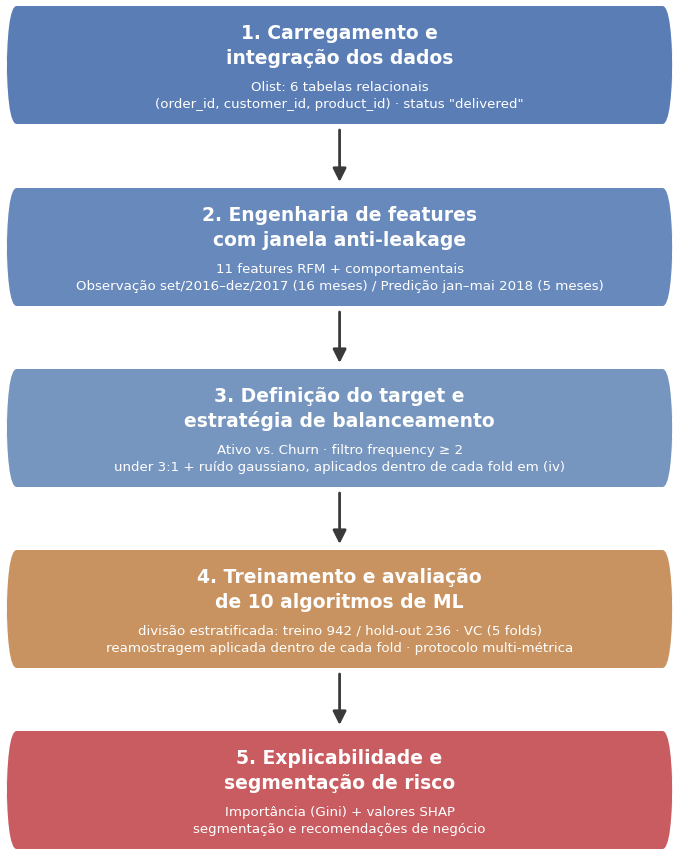
\includegraphics[width=0.6\textwidth]{USPSC-img/figuras/fig01-pipeline.png}
\end{center}
\begin{flushleft}
	\ABNTEXfontereduzida
	\SingleSpacing
	Fonte: elaborado pelo autor.

	\textit{Nota: a estratégia de balanceamento é definida na etapa (3) e aplicada na etapa (4), dentro de cada partição da validação cruzada, conforme o protocolo descrito na Seção \ref{sec:protocolo}.}
\end{flushleft}
\end{figure}

\FloatBarrier
\section{Base de Dados e Integração} \label{sec:base-dados}

A base de dados utilizada é o Olist Brazilian E-Commerce Public Dataset \cite{olist2018}, composto por seis tabelas relacionais: pedidos, clientes, itens de pedido, pagamentos, avaliações e produtos. A integração das tabelas foi realizada por meio de chaves primárias e estrangeiras compartilhadas (order\_id, customer\_id e product\_id), resultando em um dataset unificado cujo período de cobertura, conforme a documentação do conjunto de dados \cite{olist2018}, estende-se de setembro de 2016 a outubro de 2018. Foram considerados exclusivamente pedidos com status ``delivered'', garantindo que apenas transações efetivamente concluídas compusessem a base de análise.

\FloatBarrier
\section{Estratégia Temporal Anti-Leakage} \label{sec:janela-temporal}

A fim de evitar o vazamento de informação futura para o conjunto de treino, problema conhecido como data leakage, adotou-se uma estratégia de janela temporal dupla. A janela de observação, na qual as features comportamentais de cada cliente são computadas, encerra-se em 31 de dezembro de 2017 e abrange todo o histórico transacional disponível até essa data (setembro de 2016 a dezembro de 2017, aproximadamente dezesseis meses), assegurando suficiência estatística e contemplando um ciclo sazonal completo. A janela de predição, de 1.\textsuperscript{o} de janeiro a 31 de maio de 2018, define o período no qual se verifica se o cliente realizou nova compra, determinando, assim, sua classificação como Ativo (retornou) ou Churn (não retornou). Essa separação temporal garante que nenhuma informação posterior ao momento de predição influencie os modelos.

A escolha do horizonte de predição foi deliberada: cinco meses equilibram sensibilidade à recompra e representatividade do horizonte preditivo, janela compatível com um contexto de e-commerce marcado pela predominância de clientes de compra única, característica documentada para o mesmo dataset por \citeonline{matuszelanski2022}. A Figura \ref{fig:janela-temporal} representa graficamente essa separação temporal.

\begin{figure}[htbp]
\caption{Estratégia de janela temporal dupla (anti-leakage)}
\label{fig:janela-temporal}
\begin{center}
	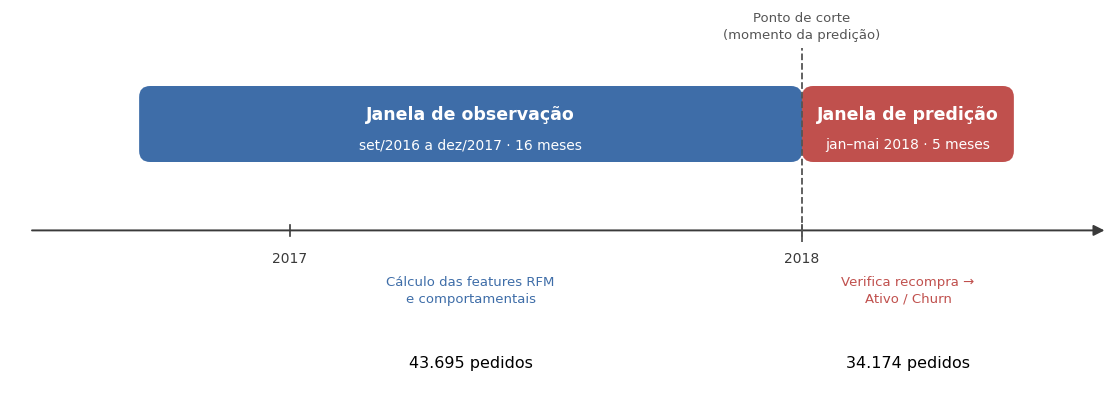
\includegraphics[width=1\textwidth]{USPSC-img/figuras/fig02-janela-temporal.png}
\end{center}
\begin{flushleft}
	\ABNTEXfontereduzida
	\SingleSpacing
	Fonte: elaborado pelo autor.
\end{flushleft}
\end{figure}

\FloatBarrier
\section{Engenharia de Features RFM} \label{sec:engenharia-features}

Com base na janela de observação, foram calculadas onze features por cliente, seguindo a metodologia RFM e incluindo variáveis complementares de comportamento transacional. A Tabela \ref{tab:features-rfm} sumariza as features construídas.

\begin{table}[htbp]
\ABNTEXfontereduzida
\SingleSpacing
\caption{Features RFM construídas na janela de observação (até dez/2017)}
\label{tab:features-rfm}
\centering
\begin{tabular}{l l l}
\hline
\textbf{Feature} & \textbf{Tipo} & \textbf{Descrição / Fórmula} \\
\hline
\textit{recency\_days}        & Numérica   & 01/01/2018 $-$ data do último pedido (em dias) \\
\textit{frequency}            & Numérica   & COUNT(DISTINCT order\_id) por customer\_unique\_id \\
\textit{monetary}             & Numérica   & SUM(valor do pedido) por customer\_unique\_id \\
\textit{avg\_ticket}          & Numérica   & monetary / frequency \\
\textit{avg\_delivery\_days}  & Numérica   & MEAN(data\_entrega $-$ data\_compra) \\
\textit{avg\_review\_score}   & Numérica   & MEAN(review\_score) \\
\textit{avg\_installments}    & Numérica   & MEAN(payment\_installments) \\
\textit{avg\_freight}         & Numérica   & MEAN(freight\_value) \\
\textit{n\_categories}        & Numérica   & COUNT(DISTINCT product\_category\_name) \\
\textit{top\_category}        & Categórica & MODE(product\_category\_name) $\rightarrow$ Label Encoding \\
\textit{customer\_state}      & Categórica & UF do cliente $\rightarrow$ Label Encoding \\
\hline
\end{tabular}
\begin{flushleft}
	\ABNTEXfontereduzida
	\SingleSpacing
	Fonte: elaborado pelo autor.

	\textit{Nota: registros sem categoria de produto identificada, correspondentes a 1,8\% do conjunto integrado, recebem o rótulo ``desconhecido'' na etapa de construção das features (Seção \ref{sec:protocolo}). Esse rótulo é computado como categoria distinta por COUNT(DISTINCT product\_category\_name), de modo que clientes com pedidos nessa condição podem ter a contagem de n\_categories acrescida em uma unidade.}
\end{flushleft}
\end{table}

As nove features numéricas cobrem as três dimensões do RFM e derivadas do comportamento transacional, conforme detalhado na Tabela \ref{tab:features-rfm}. As features categóricas compreendem top\_category e customer\_state, ambas submetidas a Label Encoding antes do treinamento. A opção pela codificação ordinal, em detrimento da codificação binária por one-hot, decorre da cardinalidade dessas variáveis frente ao tamanho da base: o catálogo de produtos do dataset contém 73 categorias distintas, às quais se soma o rótulo ``desconhecido'', de modo que a expansão binária elevaria a dimensionalidade a patamar incompatível com 1.178 observações. Cabe registrar a limitação inerente à escolha: modelos baseados em árvores tratam o inteiro atribuído a cada categoria como grandeza ordenada, produzindo partições sobre uma ordem que não possui significado substantivo. Esse efeito soma-se ao viés da importância por impureza de Gini em variáveis categóricas de cardinalidade elevada, discutido na Seção \ref{sec:interpretabilidade}, e recomenda cautela na interpretação da posição de top\_category nos rankings de importância. Codificações alternativas são registradas entre os trabalhos futuros. Clientes com frequency igual a 1 foram excluídos do escopo de modelagem, pois compradores únicos não possuem histórico suficiente para caracterizar comportamento de recompra e sua inclusão trivializaria o target Churn sem adicionar poder preditivo real.

Essa decisão de filtragem foi submetida à validação empírica no notebook que acompanha esta monografia: um modelo Random Forest de referência foi treinado em duas configurações, com o filtro adotado (frequency $\geq$ 2; 1.178 clientes) e incluindo os compradores únicos (frequency $\geq$ 1; mais de 42 mil clientes, com 98,9\% de Churn). A inclusão dos compradores únicos reduziu o ROC-AUC em aproximadamente 0,29 ponto (de 0,8106 para 0,5231), aproximando o modelo de um classificador aleatório, e degradou o MCC em cerca de 79\% (de 0,1931 para 0,0400). O resultado confirma empiricamente que os compradores únicos não agregam sinal preditivo de recompra, apenas diluem o problema, corroborando a recomendação de \citeonline{matuszelanski2022} para o dataset Olist.

A feature n\_categories foi incluída por hipótese de negócio (clientes que diversificam categorias demonstram maior engajamento com a plataforma), em linha com as recomendações de \citeonline{manzoor2024} sobre variáveis comportamentais complementares ao RFM. A variável revelou-se, posteriormente, um dos três principais drivers preditivos do modelo, em empate técnico de importância com a recência. Tal equivalência entre diversidade de categorias e recência não é reportada nos estudos anteriores aplicados ao Olist, incluindo \citeonline{matuszelanski2022}. Sua relevância sugere que a diversificação de categorias merece investigação como possível alavanca de retenção proativa, hipótese a ser confirmada em bases de maior volume.

\FloatBarrier
\section{Target e Balanceamento de Classes} \label{sec:target-balanceamento}

O target binário foi definido como: Churn = 1 para clientes que não realizaram nenhuma compra na janela de predição; e Ativo = 0 para aqueles que efetuaram ao menos uma transação no período. A base resultante apresentou desbalanceamento acentuado, com 95,8\% dos clientes classificados como Churn e 4,2\% como Ativos. Cabe destacar que essa proporção se verifica em uma coorte composta exclusivamente por clientes recorrentes, o que evidencia que, mesmo entre consumidores com histórico de recompra, os intervalos entre transações tendem a exceder o horizonte de predição adotado, característica consistente com a baixa taxa de retorno documentada para o dataset Olist \cite{matuszelanski2022}.

Para mitigar o efeito do desbalanceamento extremo, que tende a produzir modelos enviesados para a classe majoritária e com baixa capacidade preditiva real \cite{he2009}, adotou-se uma estratégia combinada de under e oversampling aplicada exclusivamente ao conjunto de treino. O undersampling reduziu a classe majoritária (Churn) a no máximo três vezes o tamanho da classe minoritária (Ativo). O oversampling sintético por ruído gaussiano de média zero e desvio-padrão 0,05, aplicado sobre as features já padronizadas (média 0, desvio padrão 1), expandiu a classe Ativo até igualar o tamanho da maioria, produzindo um conjunto de treino perfeitamente balanceado. Não se trata de interpolação entre vizinhos, como no SMOTE: cada instância sintética é uma cópia de uma observação real da classe minoritária somada a perturbação de baixa magnitude, procedimento que preserva a vizinhança original em vez de criar pontos em regiões não observadas do espaço de features. O procedimento corresponde à replicação ruidosa (\textit{noisy replication}) formulada por \citeonline{lee2000} para classificação binária com classes assimétricas, e encontra respaldo teórico no resultado de \citeonline{bishop1995}, segundo o qual o treinamento com ruído aditivo de baixa variância equivale a uma forma de regularização de Tikhonov, o que explica por que a perturbação atua como regularizador em vez de introduzir ruído estrutural. O conjunto de teste foi mantido com a distribuição original, preservando a validade da avaliação.

Essa escolha se apoiou em uma análise comparativa sistemática das alternativas de tratamento do desbalanceamento, sintetizada no Quadro \ref{qua:estrategias-balanceamento}, que pondera vantagens e riscos de cada estratégia à luz do tamanho reduzido da classe minoritária (aproximadamente 50 clientes ativos). Optou-se pela combinação de undersampling moderado (razão 3:1) com oversampling gaussiano por preservar a vizinhança real dos dados sem descartar informação da classe majoritária nem gerar instâncias em regiões não representativas, como poderia ocorrer com o SMOTE \cite{chawla2002} em um conjunto tão pequeno e esparso. Trata-se, portanto, de alternativa deliberadamente mais conservadora, cuja adequação foi verificada empiricamente por meio da análise de representatividade conduzida na Seção \ref{sec:representatividade}.

\begin{quadro}[htbp]
\ABNTEXfontereduzida
\SingleSpacing
\caption{Análise comparativa de estratégias de balanceamento de classes}
\label{qua:estrategias-balanceamento}
\centering
\begin{tabular}{|>{\raggedright\arraybackslash}p{3.0cm}|>{\raggedright\arraybackslash}p{5.3cm}|>{\raggedright\arraybackslash}p{5.6cm}|}
\hline
\textbf{Estratégia} & \textbf{Vantagens} & \textbf{Desvantagens / Riscos} \\
\hline
Sem balanceamento & Preserva a distribuição real; sem artefatos sintéticos. & Modelos enviesados para a classe majoritária, com regra de decisão que só alcança recall não trivial na classe Ativo mediante limiar muito acima do padrão (0,75 na Tabela \ref{tab:comparacao-balanceamento}). \\
\hline
Undersampling puro & Simples; reduz custo computacional; sem dados sintéticos. & Descarta a quase totalidade da classe Churn; base de treino diminuta (cerca de 80 amostras) com 40 Ativos. \\
\hline
SMOTE (oversampling sintético) & Amplia a classe minoritária por interpolação entre vizinhos reais; consagrado na literatura. & Em datasets pequenos e esparsos, gera instâncias em regiões não representativas; risco de ruído estrutural. \\
\hline
\textbf{Under + oversampling gaussiano (adotada)} & Equilibra as classes; retém três vezes mais amostras Churn que o undersampling puro; perturbação de baixa magnitude preserva a vizinhança real. & Ainda descarta cerca de 87\% da classe Churn presente no conjunto de treino; dois terços da classe Ativo no treino são sintéticos; exige validação de representatividade (Seção \ref{sec:representatividade}). \\
\hline
\end{tabular}
\begin{flushleft}
	\ABNTEXfontereduzida
	\SingleSpacing
	Fonte: elaborado pelo autor.
\end{flushleft}
\end{quadro}

\begin{table}[htbp]
\ABNTEXfontereduzida
\SingleSpacing
\caption{Comparação empírica de estratégias de balanceamento (split de referência)}
\label{tab:comparacao-balanceamento}
\centering
\scriptsize
\setlength{\tabcolsep}{3pt}
\begin{tabular}{@{}>{\raggedright\arraybackslash}p{3.0cm}rrrrrrrrr@{}}
\hline
\textbf{Estratégia} & \shortstack[r]{\textbf{N}\\\textbf{treino}} & \shortstack[r]{\textbf{ROC-}\\\textbf{AUC}} & \shortstack[r]{\textbf{CV-}\\\textbf{AUC}} & \textbf{MCC} & \textbf{Kappa} & \shortstack[r]{\textbf{F1-}\\\textbf{Macro}} & \shortstack[r]{\textbf{Rec.}\\\textbf{Ativo}} & \shortstack[r]{\textbf{Rec.}\\\textbf{Churn}} & \textbf{Limiar} \\
\hline
Sem balanceamento & 942 & 0,8018 & 0,6017 & 0,2983 & 0,2680 & 0,6319 & 0,20 & 0,9912 & 0,75 \\
Undersampling puro (1:1) & 80 & 0,7451 & 0,6080 & 0,1943 & 0,1884 & 0,5930 & 0,30 & 0,9425 & 0,27 \\
SMOTE & 1.804 & 0,7327 & 0,5928 & 0,1253 & 0,1233 & 0,5610 & 0,20 & 0,9469 & 0,44 \\
\textbf{Under 3:1 + gaussiano (adotada)} & \textbf{240} & \textbf{0,8106} & \textbf{0,6814} & \textbf{0,1931} & \textbf{0,1918} & \textbf{0,5957} & \textbf{0,20} & \textbf{0,9735} & \textbf{0,38} \\
\hline
\end{tabular}
\begin{flushleft}
	\ABNTEXfontereduzida
	\SingleSpacing
	Fonte: elaborado pelo autor.

	\textit{Nota: modelo de referência Random Forest (n\_estimators = 300, max\_depth = 10), mantido fixo nas quatro estratégias; o que se compara aqui são estratégias de reamostragem, não algoritmos. A reamostragem é aplicada dentro de cada partição da validação cruzada, e o limiar de classificação é derivado das probabilidades out-of-fold do conjunto de treino, conforme o protocolo descrito na Seção \ref{sec:protocolo}. Como o limiar é derivado independentemente em cada estratégia, as métricas dependentes de limiar (MCC, Kappa, F1-Macro e os recalls) são calculadas em pontos de corte distintos e não constituem comparação direta entre estratégias; a comparação estritamente pareada é a das colunas ROC-AUC e CV-AUC.}
\end{flushleft}
\end{table}

\begin{table}[htbp]
\ABNTEXfontereduzida
\SingleSpacing
\caption{Robustez das estratégias de balanceamento em trinta divisões estratificadas}
\label{tab:robustez-balanceamento}
\centering
\scriptsize
\setlength{\tabcolsep}{4pt}
\begin{tabular}{@{}>{\raggedright\arraybackslash}p{4.0cm}rrrr@{}}
\hline
\textbf{Estratégia} & \shortstack[r]{\textbf{ROC-AUC}\\\textbf{média}} & \shortstack[r]{\textbf{MCC}\\\textbf{médio}} & \shortstack[r]{\textbf{Kappa}\\\textbf{médio}} & \shortstack[r]{\textbf{Amplitude da}\\\textbf{ROC-AUC}} \\
\hline
Sem balanceamento & 0,6543 $\pm$ 0,0778 & 0,1168 $\pm$ 0,1167 & 0,1031 $\pm$ 0,1004 & 0,462 - 0,800 \\
Undersampling puro (1:1) & 0,6510 $\pm$ 0,0769 & 0,0439 $\pm$ 0,0765 & 0,0392 $\pm$ 0,0689 & 0,501 - 0,802 \\
SMOTE & 0,6615 $\pm$ 0,0660 & 0,1060 $\pm$ 0,0761 & 0,0895 $\pm$ 0,0696 & 0,539 - 0,810 \\
\textbf{Under 3:1 + gaussiano (adotada)} & \textbf{0,6686 $\pm$ 0,0831} & \textbf{0,1140 $\pm$ 0,0804} & \textbf{0,1053 $\pm$ 0,0726} & \textbf{0,500 - 0,822} \\
\hline
\end{tabular}
\begin{flushleft}
	\ABNTEXfontereduzida
	\SingleSpacing
	Fonte: elaborado pelo autor.

	\textit{Nota: aplica-se aqui a mesma observação da Tabela \ref{tab:comparacao-balanceamento} quanto ao modelo de referência e ao protocolo de avaliação.}
\end{flushleft}
\end{table}

A comparação empírica das quatro estratégias, conduzida no notebook que acompanha esta monografia e sintetizada nas Tabelas \ref{tab:comparacao-balanceamento} e \ref{tab:robustez-balanceamento}, corrobora a escolha adotada. No split de referência, a combinação de undersampling moderado com oversampling gaussiano obteve a maior ROC-AUC (0,811), à frente da ausência de balanceamento (0,802), do undersampling puro (0,745) e do SMOTE (0,733). Para verificar se esse resultado não decorria de uma partição favorável, o experimento foi repetido em trinta divisões estratificadas independentes, nas quais a estratégia adotada manteve a maior ROC-AUC média (0,669), seguida pelo SMOTE (0,662), pela ausência de balanceamento (0,654) e pelo undersampling puro (0,651).

O desempenho inferior do undersampling puro é consistente com a redução drástica do conjunto de treino que a estratégia impõe: com apenas 40 clientes Ativos no treino, o balanceamento 1:1 produz 80 amostras, base insuficiente para algoritmos ensemble. O SMOTE \cite{chawla2002}, por sua vez, interpola entre vizinhos reais, procedimento que em conjuntos pequenos e esparsos tende a gerar instâncias em regiões pouco representativas do espaço de features. A ausência de balanceamento, embora competitiva em ROC-AUC, preserva o viés estrutural para a classe majoritária que a literatura documenta em cenários de desbalanceamento extremo \cite{he2009}.

Cabe registrar duas ressalvas. A primeira é que, segundo o Coeficiente de Correlação de Matthews, uma das três métricas recomendadas por De la Cruz Huayanay, Bazán e Russo (\citeyear{delacruz2025}), a ausência de balanceamento supera a estratégia adotada no split de referência (0,2983 contra 0,1931, Tabela \ref{tab:comparacao-balanceamento}). O mesmo se verifica no Kappa de Cohen (0,2680 contra 0,1918) e no F1-Macro (0,6319 contra 0,5957), ambos igualmente favoráveis à ausência de balanceamento nesse split. Cabe observar, contudo, que essa vantagem não se traduz em ganho na classe minoritária: ambas as estratégias identificam corretamente a mesma proporção de clientes Ativos (Recall-Ativo de 0,20), e a diferença de MCC decorre exclusivamente do desempenho na classe majoritária (Recall-Churn de 0,9912 contra 0,9735). Na média das trinta divisões independentes, a diferença praticamente desaparece (MCC de 0,1140 para a estratégia adotada contra 0,1168 para a ausência de balanceamento, com desvios-padrão de 0,0804 e 0,1167), e a estratégia adotada apresenta o maior Kappa médio do conjunto (0,1053). A segunda ressalva é que as diferenças entre as estratégias situam-se dentro de um desvio-padrão, de modo que os resultados indicam tendência, e não superioridade estatisticamente estabelecida. A amplitude da ROC-AUC entre divisões, de 0,500 a 0,822 para a estratégia adotada, decorre do tamanho reduzido da classe Ativo no conjunto de teste (aproximadamente dez instâncias), limitação inerente ao problema e discutida ao longo deste trabalho. Reconhece-se, por fim, que o oversampling por ruído amplia a classe minoritária a partir de uma base amostral reduzida, o que motiva a análise de representatividade conduzida na Seção \ref{sec:representatividade}.

\FloatBarrier
\section{Protocolo de Treinamento e Avaliação} \label{sec:protocolo}

Os dados foram divididos em treino (80\%) e teste (20\%) por meio de StratifiedShuffleSplit, garantindo a proporção original de classes em ambos os conjuntos. A imputação de valores ausentes no conjunto de modelagem foi realizada pela mediana das features numéricas, e a padronização foi aplicada via StandardScaler, com parâmetros ajustados exclusivamente no conjunto de treino para evitar contaminação do teste \cite{kaufman2012}.

Precede essa etapa o tratamento de ausências na construção das features, integralmente contido na janela de observação e, portanto, anterior à definição do target e sem acesso a informação da janela de predição. Nesse tratamento, as variáveis de valor de pagamento e de avaliação foram imputadas pela mediana da respectiva coluna; as variáveis de frete e de número de parcelas receberam os valores neutros zero e um; e a categoria do produto, ausente em 1,8\% dos registros do conjunto integrado, recebeu o rótulo ``desconhecido'', conforme registrado na nota da Tabela \ref{tab:features-rfm}.

Foram treinados e avaliados dez algoritmos de Machine Learning: Regressão Logística, Árvore de Decisão, Random Forest, Extra Trees, Gradient Boosting, HistGradient Boosting, AdaBoost, K-Nearest Neighbors (KNN), Gaussian Naive Bayes e Support Vector Machine (SVM). Cada modelo foi submetido a validação cruzada estratificada com cinco folds (StratifiedKFold) no conjunto de treino e avaliado no hold-out de teste. A imputação, a padronização e a reamostragem são ajustadas dentro de cada partição, exclusivamente sobre a porção de ajuste, procedimento necessário para que instâncias sintéticas derivadas de uma mesma observação original não se distribuam entre folds distintos \cite{hastie2009,kaufman2012}. Registra-se que parte dos estimadores mantém o parâmetro class\_weight = ``balanced'' por padrão defensivo; sob o conjunto de treino perfeitamente balanceado (120/120), o parâmetro atribui pesos iguais às classes e é, portanto, neutro.

O protocolo de avaliação adota um conjunto abrangente de métricas sensíveis ao desbalanceamento, incorporando as três recomendadas por De la Cruz Huayanay, Bazán e Russo (\citeyear{delacruz2025}), a saber, MCC (Coeficiente de Correlação de Matthews), G-Mean e Kappa de Cohen, além de ROC-AUC, Average Precision, F1-Macro, Precisão e Recall por classe. Adota-se a classe Churn como positiva em todas as métricas por classe e na leitura da matriz de confusão, de modo que falso positivo designa cliente Ativo classificado como Churn, e falso negativo, cliente Churn classificado como Ativo.

O limiar de classificação constitui parâmetro livre da regra de decisão e, como tal, deve ser estimado sobre dados que não participem do relato de desempenho; estimá-lo no conjunto de teste equivale a utilizá-lo duas vezes, uma para ajustar o parâmetro e outra para reportar o resultado, o que caracteriza viés de seleção na avaliação \cite{cawley2010,hastie2009}. Dado que o valor padrão de 0,50 raramente é ótimo \cite{fawcett2006} e que o tamanho da classe minoritária inviabiliza a extração de uma terceira partição de validação, adotou-se o seguinte procedimento: as probabilidades preditas foram obtidas por validação cruzada estratificada de cinco folds sobre o conjunto de treino, com a reamostragem aplicada exclusivamente à porção de ajuste de cada partição e a porção de validação mantida na distribuição original das classes; sobre essas probabilidades out-of-fold, agregadas, o limiar foi varrido uma única vez no intervalo de 0,01 a 0,99, selecionando-se o valor que maximiza o Kappa de Cohen, mesmo critério adotado por De la Cruz Huayanay, Bazán e Russo (\citeyear{delacruz2025}). O limiar assim obtido foi congelado e aplicado ao hold-out, que permanece utilizado uma única vez. Como as probabilidades out-of-fold são estimadas sob a prevalência original, o limiar transfere-se ao conjunto de teste sem necessidade de correção adicional pelo viés de amostragem formalizado por \citeonline{dalpozzolo2015}. A escolha do Kappa de Cohen como critério de varredura mostrou-se pouco sensível: em oito dos dez algoritmos avaliados, incluindo o Random Forest adotado como modelo de produção, o limiar selecionado coincide com o que resultaria da maximização do F1-Macro. Divergem apenas o SVM, cujo limiar passaria de 0,37 para 0,23, e a Árvore de Decisão, de 0,61 para 0,01.

O critério de seleção do modelo de produção foi reformulado em relação à concepção inicial deste trabalho. A verificação de sobreajuste pela diferença entre validação cruzada e hold-out, conduzida sob o protocolo corrigido descrito acima, não excluiu nenhum dos dez algoritmos: a maior diferença observada foi de 0,1347 (Árvore de Decisão), abaixo do limite de 0,15 fixado para esta verificação. A prática de contrastar a estimativa reamostrada com a de um conjunto reservado, como diagnóstico do otimismo introduzido pelo procedimento de seleção, é recomendada por \citeonline{hastie2009} e por \citeonline{cawley2010}, que não estabelecem, contudo, um valor numérico de corte. O limite de 0,15 é, portanto, um parâmetro operacional definido por este trabalho antes da execução do benchmark, cuja função é tornar o critério auditável, e não uma grandeza extraída da literatura. A sensibilidade a essa escolha é reportada na Seção \ref{sec:benchmark}. Os valores elevados de validação cruzada obtidos na concepção inicial decorriam do procedimento então adotado, no qual a validação era conduzida sobre o conjunto já balanceado; a magnitude da correção é reportada na Seção \ref{sec:benchmark}. A seleção passou, assim, a fundamentar-se na natureza do entregável, discutida na Seção \ref{sec:benchmark} e detalhada na Seção \ref{sec:segmentacao}: o produto do modelo não é uma decisão binária em um ponto de corte, mas uma priorização de clientes em faixas de risco, que depende da ordenação dos scores e não do limiar. Por essa razão, o critério primário adotado é a qualidade da ordenação, medida por ROC-AUC e Average Precision, complementado pela verificação da eficiência do recorte resultante em cobertura fixa e pela disponibilidade de medidas nativas de importância de features, requisito do objetivo específico (\ref{obj:importancia}).

Todas as operações estocásticas do pipeline, incluindo divisão treino/teste, balanceamento e treinamento dos modelos, utilizam semente fixa (random\_state = 42), garantindo reprodutibilidade exata dos resultados em uma mesma configuração de ambiente; excetua-se a análise de robustez apresentada na Seção \ref{sec:target-balanceamento}, que varia deliberadamente a semente de particionamento. Cabe registrar, contudo, que a fixação de semente assegura determinismo apenas dentro de uma mesma versão das bibliotecas: alterações de implementação interna entre versões do scikit-learn \cite{pedregosa2011} podem produzir variações marginais nas métricas e na ordenação de features de importância próxima, sem comprometer as conclusões qualitativas do estudo. Os valores reportados neste trabalho correspondem à execução de referência documentada no notebook que acompanha esta monografia, disponível no repositório do autor \cite{ugulino2026}. O repositório contém o código integral do pipeline, as saídas de cada etapa na execução de referência e o arquivo de ambiente com as versões das bibliotecas utilizadas. O conjunto de dados não é redistribuído; sua origem é a indicada em \citeonline{olist2018}.

\FloatBarrier


\chapter{Avaliação Experimental} \label{Cap:AvaliacaoExperimental}

\FloatBarrier
\section{Análise Exploratória dos Dados} \label{sec:eda}

A análise exploratória revelou padrões comportamentais consistentes com a literatura de churn em e-commerce de varejo \cite{matuszelanski2022}. A distribuição de recência demonstra que clientes Ativos situam-se majoritariamente nos primeiros cem dias desde a última compra (66\% dos casos), com média de 84 dias, enquanto clientes Churn apresentam distribuição mais dispersa, com média de 126 dias e ocorrências isoladas que ultrapassam 400 dias de ausência. Essa separação confirma a recência, uma das dimensões centrais do framework RFM \cite{hughes1994}, como variável com poder discriminativo relevante.

A análise de frequência, segunda dimensão do RFM, evidencia que ambas as classes apresentam mediana de dois pedidos, mínimo imposto pelo filtro adotado, mas os clientes Ativos exibem média superior (2,56 contra 2,08 pedidos), com maior dispersão e valores extremos de até oito pedidos, contra seis entre os Churn. O review score médio apresenta diferença marginal entre as classes (Ativos: 4,25; Churn: 4,21), sugerindo que a satisfação declarada não é fator determinante isolado para a retenção, indicação de que o churn configura-se como um problema de engajamento, e não de qualidade do serviço \cite{manzoor2024}.

O perfil comparativo multivariado confirma que as dimensões mais discriminativas entre Ativos e Churn são o valor monetário total, terceira dimensão do RFM \cite{hughes1994}, com média de R\$ 372,25 entre os Ativos contra R\$ 299,12 entre os Churn, e o número de categorias distintas, indicador de engajamento não capturado pelo RFM puro \cite{manzoor2024}, com média de 1,80 categorias entre os Ativos contra 1,54 entre os Churn. O ticket médio (R\$ 150,70 contra R\$ 143,97), assim como o tempo de entrega e o review score, não apresentou separação expressiva entre as classes nesta análise univariada, indicando menor relevância preditiva isolada dessas variáveis.

A Figura \ref{fig:eda-recencia} evidencia a concentração dos clientes Ativos em intervalos curtos desde a última compra, enquanto os clientes Churn dispersam-se por períodos mais longos. A Figura \ref{fig:eda-frequencia} mostra medianas idênticas de dois pedidos, com os Ativos apresentando maior dispersão e valores extremos superiores. A Figura \ref{fig:eda-review} confirma a diferença marginal de review score entre as classes. A Figura \ref{fig:proporcao-classes} explicita o desbalanceamento de 95,8\% contra 4,2\%.

\begin{figure}[htbp]
\caption{Análise exploratória de recência}
\label{fig:eda-recencia}
\begin{center}
	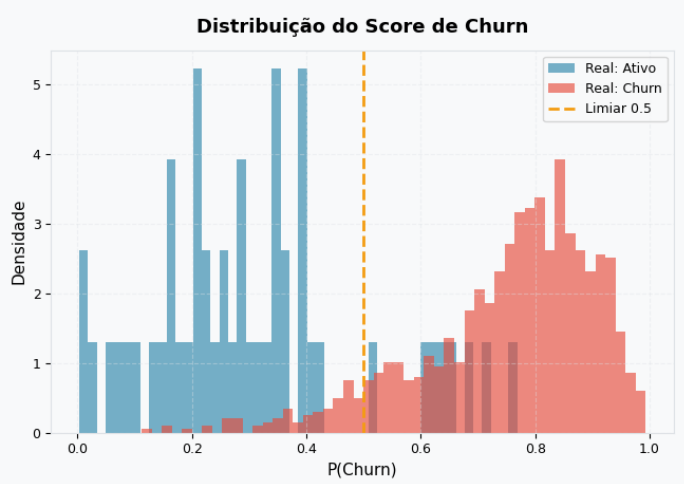
\includegraphics[width=0.9\textwidth]{USPSC-img/figuras/fig03-eda-recencia.png}
\end{center}
\begin{flushleft}
	\ABNTEXfontereduzida
	\SingleSpacing
	Fonte: elaborado pelo autor.
\end{flushleft}
\end{figure}

\begin{figure}[htbp]
\caption{Análise exploratória de frequência}
\label{fig:eda-frequencia}
\begin{center}
	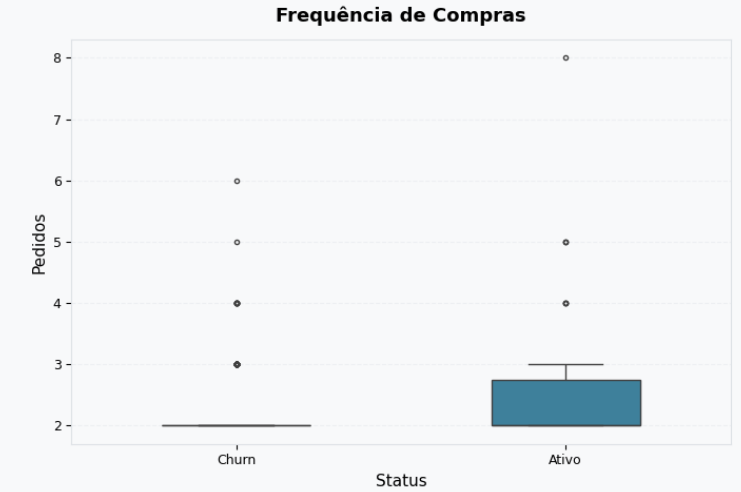
\includegraphics[width=0.9\textwidth]{USPSC-img/figuras/fig04-eda-frequencia.png}
\end{center}
\begin{flushleft}
	\ABNTEXfontereduzida
	\SingleSpacing
	Fonte: elaborado pelo autor.
\end{flushleft}
\end{figure}

\begin{figure}[htbp]
\caption{Análise exploratória de review score}
\label{fig:eda-review}
\begin{center}
	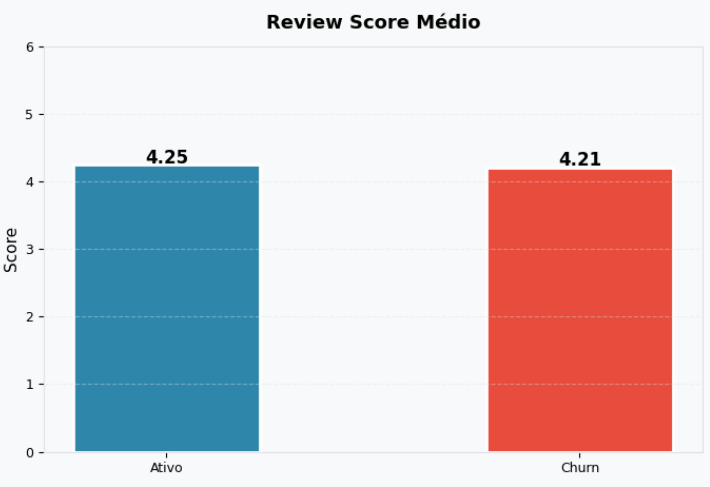
\includegraphics[width=0.9\textwidth]{USPSC-img/figuras/fig05-eda-review-score.png}
\end{center}
\begin{flushleft}
	\ABNTEXfontereduzida
	\SingleSpacing
	Fonte: elaborado pelo autor.
\end{flushleft}
\end{figure}

\begin{figure}[htbp]
\caption{Proporção Churn versus Ativo}
\label{fig:proporcao-classes}
\begin{center}
	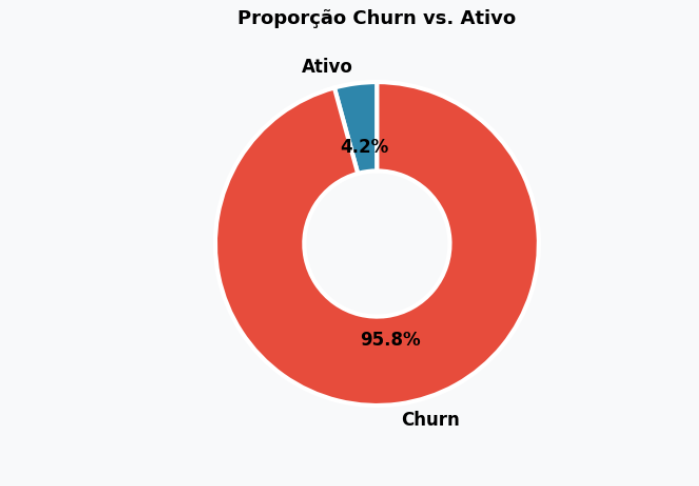
\includegraphics[width=0.7\textwidth]{USPSC-img/figuras/fig06-proporcao-churn-ativo.png}
\end{center}
\begin{flushleft}
	\ABNTEXfontereduzida
	\SingleSpacing
	Fonte: elaborado pelo autor.
\end{flushleft}
\end{figure}

\FloatBarrier
\section{Benchmark Comparativo de Algoritmos} \label{sec:benchmark}

A Tabela \ref{tab:benchmark} apresenta os resultados consolidados dos dez algoritmos avaliados, ordenados por ROC-AUC no conjunto de teste e acompanhados das métricas complementares MCC, G-Mean e Kappa, cujos rankings são analisados na Seção \ref{sec:correlacao-rankings}. O Random Forest obteve o melhor desempenho em termos de discriminação global (AUC = 0,8106), seguido pelo HistGradient Boosting (AUC = 0,7615) e pelo Extra Trees (AUC = 0,7491). No extremo oposto, a Árvore de Decisão apresentou o pior resultado (AUC = 0,4772), valor inferior ao do classificador aleatório, cujo AUC teórico é 0,50 \cite{fawcett2006}, seguida pelo KNN (AUC = 0,5336). Em ambos os casos, o desempenho aproxima-se ou situa-se abaixo do classificador aleatório, resultado discutido adiante à luz do protocolo de validação adotado.

\begin{table}[htbp]
\ABNTEXfontereduzida
\SingleSpacing
\caption{Benchmark comparativo dos dez algoritmos de Machine Learning}
\label{tab:benchmark}
\centering
\scriptsize
\setlength{\tabcolsep}{2.2pt}
\begin{tabular}{@{}>{\raggedright\arraybackslash}p{2.3cm}rrrrrrrrrrrr@{}}
\hline
\textbf{Modelo} & \textbf{AUC} & \textbf{AP} & \shortstack[r]{\textbf{CV-}\\\textbf{AUC}} & \textbf{$\Delta$} & \shortstack[r]{\textbf{F1-}\\\textbf{Macro}} & \textbf{MCC} & \shortstack[r]{\textbf{G-}\\\textbf{Mean}} & \textbf{Kappa} & \shortstack[r]{\textbf{Prec.}\\\textbf{Ativo}} & \shortstack[r]{\textbf{Rec.}\\\textbf{Ativo}} & \shortstack[r]{\textbf{Rec.}\\\textbf{Churn}} & \textbf{Limiar} \\
\hline
Random Forest & 0,8106 & 0,9905 & 0,6814 & 0,1293 & 0,5957 & 0,1931 & 0,4412 & 0,1918 & 0,2500 & 0,20 & 0,9735 & 0,38 \\
HistGradient Boosting & 0,7615 & 0,9872 & 0,7363 & 0,0252 & 0,6049 & 0,2143 & 0,5342 & 0,2110 & 0,2143 & 0,30 & 0,9513 & 0,18 \\
Extra Trees & 0,7491 & 0,9860 & 0,6777 & 0,0714 & 0,5649 & 0,1639 & 0,3148 & 0,1370 & 0,3333 & 0,10 & 0,9912 & 0,34 \\
Regressão Logística & 0,7075 & 0,9838 & 0,6326 & 0,0749 & 0,6440 & 0,3517 & 0,4462 & 0,2939 & 0,6667 & 0,20 & 0,9956 & 0,12 \\
SVM & 0,7035 & 0,9833 & 0,6238 & 0,0798 & 0,4920 & 0,0250 & 0,4111 & 0,0197 & 0,0541 & 0,20 & 0,8451 & 0,37 \\
Gradient Boosting & 0,6642 & 0,9796 & 0,6695 & 0,0053 & 0,5339 & 0,0679 & 0,3106 & 0,0678 & 0,1111 & 0,10 & 0,9646 & 0,08 \\
Naive Bayes & 0,6405 & 0,9552 & 0,6390 & 0,0015 & 0,5887 & 0,1778 & 0,4402 & 0,1775 & 0,2222 & 0,20 & 0,9690 & 0,01 \\
AdaBoost & 0,5544 & 0,9694 & 0,5372 & 0,0172 & 0,5725 & 0,2100 & 0,3155 & 0,1547 & 0,5000 & 0,10 & 0,9956 & 0,47 \\
KNN & 0,5336 & 0,9596 & 0,5913 & 0,0577 & 0,5143 & 0,0314 & 0,3063 & 0,0307 & 0,0667 & 0,10 & 0,9381 & 0,09 \\
Árvore de Decisão & 0,4772 & 0,9559 & 0,6119 & 0,1347 & 0,4592 & 0,0178 & 0,4708 & 0,0112 & 0,0484 & 0,30 & 0,7389 & 0,61 \\
\hline
\end{tabular}
\begin{flushleft}
	\ABNTEXfontereduzida
	\SingleSpacing
	Fonte: elaborado pelo autor.

	\textit{Nota: $\Delta$ é a diferença absoluta entre CV-AUC e AUC no hold-out. AP designa a Average Precision para a classe Churn, cuja linha de base no conjunto de teste é 0,958, valor correspondente à prevalência dessa classe; a informação relevante nessa coluna é a comparação entre modelos, e não a magnitude absoluta. Rec. Ativo corresponde à proporção das dez instâncias da classe Ativo do conjunto de teste corretamente identificadas. O limiar de cada modelo foi derivado das probabilidades out-of-fold do conjunto de treino, conforme a Seção \ref{sec:protocolo}, e todas as métricas dependentes de limiar foram calculadas nesse valor. Nenhum modelo foi descartado pelo critério de diferença entre validação cruzada e hold-out.}
\end{flushleft}
\end{table}

A validação cruzada, conduzida com a reamostragem aplicada dentro de cada partição, não indicou sobreajuste em nenhum dos dez algoritmos: a maior diferença em relação ao hold-out foi de 0,1347 (Árvore de Decisão), seguida de 0,1293 (Random Forest), ambas abaixo do limite de 0,15 fixado na Seção \ref{sec:protocolo}. Registra-se a sensibilidade a esse parâmetro: sob um corte de 0,10, esses dois algoritmos seriam descartados, entre eles o adotado como modelo de produção; sob 0,20, o resultado seria idêntico ao obtido. Como nenhum modelo foi excluído pelo critério, ele não participou da escolha do modelo de produção, que se apoia nos fundamentos expostos adiante nesta seção. Esse resultado contrasta com o obtido na concepção inicial deste trabalho, em que a validação cruzada era conduzida sobre o conjunto de treino já balanceado. Naquele protocolo, instâncias sintéticas geradas por perturbação de uma mesma observação original distribuíam-se entre folds distintos, e o modelo avaliava, na partição de validação, quase duplicatas de exemplos vistos no ajuste. O efeito da correção é sistemático e ordena-se pela capacidade de memorização de cada algoritmo: a estimativa de validação cruzada caiu 0,3251 no AdaBoost, 0,3222 no KNN e 0,2657 no Extra Trees, contra apenas 0,0789 na Regressão Logística e 0,0634 no Naive Bayes, modelos paramétricos cuja estrutura não permite memorizar instâncias próximas. O caso do KNN é ilustrativo: sua estimativa de validação cruzada passou de 0,9135 para 0,5913, valor compatível com o desempenho de 0,5336 obtido no hold-out. Conclui-se que a diferença entre validação cruzada e hold-out observada na concepção inicial media vazamento de informação entre partições, e não sobreajuste ao conjunto de treino.

Sob as três métricas recomendadas por De la Cruz Huayanay, Bazán e Russo (\citeyear{delacruz2025}), o modelo indicado seria o HistGradient Boosting: ele lidera o G-Mean (0,5342, o maior valor do conjunto) e ocupa a segunda posição em MCC (0,2143) e em Kappa de Cohen (0,2110). É também um dos dois algoritmos que identificam o maior número de clientes Ativos, três das dez instâncias do hold-out, empatado com a Árvore de Decisão mas com precisão muito superior (0,2143 contra 0,0484), e o que apresenta a menor diferença entre validação cruzada e hold-out entre os três modelos de melhor desempenho (0,0252), além da maior CV-AUC do conjunto (0,7363). A liderança isolada em MCC (0,3517) e Kappa (0,2939) cabe, contudo, à Regressão Logística, cuja vantagem não se sustenta na classe minoritária: o modelo identifica as mesmas duas instâncias Ativas que o Random Forest, e sua superioridade decorre integralmente da redução de falsos negativos, isto é, de clientes Churn incorretamente classificados como Ativos (um caso contra seis). Trata-se do mesmo padrão registrado na Seção \ref{sec:target-balanceamento} a respeito da ausência de balanceamento. O Random Forest, por sua vez, lidera a ROC-AUC (0,8106) e a Average Precision para a classe Churn (0,9905), as duas métricas do conjunto que independem do limiar de classificação e que medem, portanto, a qualidade da ordenação dos clientes por risco.

Os valores absolutos de MCC e Kappa de Cohen, com máximos de 0,35 e 0,29 respectivamente entre os dez modelos, situam-se abaixo do limiar usualmente associado a concordância substancial \cite{landis1977}. É importante enfatizar que essa limitação decorre estruturalmente da composição do conjunto de teste: com apenas dez instâncias da classe Ativo em um hold-out de 236 clientes, no qual a proporção de 4,2\% da base foi preservada, qualquer erro de classificação na classe minoritária impacta desproporcionalmente o MCC e o Kappa, comportamento previsto analiticamente por \citeonline{luque2019} e coerente com a sensibilidade do MCC a todos os quadrantes da matriz de confusão, destacada por \citeonline{chicco2020}. A mesma escassez restringe o número de configurações possíveis da matriz de confusão: o Recall da classe Ativo assume apenas três valores distintos entre os dez algoritmos avaliados (0,10, 0,20 e 0,30), e nenhum modelo ultrapassa três acertos em dez. Não se trata de falha algorítmica, mas de consequência matemática do desbalanceamento extremo preservado no hold-out, escolha metodológica deliberada para preservar a validade da avaliação em condições reais de operação.

Os três modelos de melhor desempenho, Random Forest, HistGradient Boosting e Regressão Logística, apresentam perfis distintos de vantagens e desvantagens, sintetizados no Quadro \ref{qua:tres-modelos}. A inclusão da Regressão Logística no quadro decorre de sua liderança isolada em MCC e Kappa de Cohen: sob as métricas recomendadas por De la Cruz Huayanay, Bazán e Russo (\citeyear{delacruz2025}), ela é candidata obrigatória, ainda que a literatura a trate como modelo de referência e não como concorrente dos ensembles \cite{prabadevi2023}. A escolha entre os três não é absoluta, mas está condicionada ao objetivo do negócio e à estrutura de custos da operação de retenção.

\begingroup
% Reserva espaco para que a legenda nao fique separada da primeira linha do quadro
\Needspace*{10\baselineskip}
\quadrocaption{Análise de vantagens e desvantagens dos três modelos de melhor desempenho}
\label{qua:tres-modelos}
\ABNTEXfontereduzida
\SingleSpacing
\begin{longtable}{|>{\raggedright\arraybackslash}p{2.3cm}|>{\raggedright\arraybackslash}p{5.6cm}|>{\raggedright\arraybackslash}p{5.6cm}|}
\hline
\textbf{Modelo} & \textbf{Vantagens} & \textbf{Desvantagens} \\
\hline
\endfirsthead
\hline
\textbf{Modelo} & \textbf{Vantagens} & \textbf{Desvantagens} \\
\hline
\endhead
\hline
\endfoot
\hline
\endlastfoot
Random Forest (produção) &
Maior ROC-AUC (0,8106) e maior Average Precision para a classe Churn (0,9905), as duas métricas que independem do limiar e medem a qualidade da ordenação dos clientes por risco; melhor captura de clientes Ativos em cobertura fixa, liderando ou empatando em todas as frações avaliadas entre 10\% e 60\% do conjunto de teste; alcança 90\% dos clientes Ativos abordando 35,6\% das observações, a menor cobertura entre os três modelos; retém nove dos dez clientes Ativos do conjunto de teste fora da faixa Crítico, em 39,0\% das observações, lift de 2,31 vezes; importância de features nativa via impureza de Gini, requisito do objetivo específico (\ref{obj:importancia}). &
Menores MCC (0,1931), Kappa de Cohen (0,1918) e G-Mean (0,4412) entre os três modelos; identifica duas das dez instâncias Ativas do hold-out, contra três do HistGradient Boosting; menor Average Precision para a classe Ativo (0,1494, contra 0,2559 do HistGradient Boosting), métrica dominada pelo extremo inicial da ordenação; maior diferença entre validação cruzada e hold-out entre os três (0,1293); ROC-AUC média em validação cruzada de 0,6814, inferior aos 0,7363 do HistGradient Boosting; maior custo de memória em produção. \\
\hline
HistGradient Boosting (alternativo) &
Lidera o G-Mean (0,5342, o maior valor do conjunto de dez algoritmos); segundo maior MCC (0,2143) e Kappa de Cohen (0,2110); identifica três das dez instâncias Ativas do hold-out, o maior número entre os três modelos; maior Average Precision para a classe Ativo entre os três (0,2559), o que indica acerto no extremo inicial da ordenação; maior CV-AUC do conjunto (0,7363) e menor diferença em relação ao hold-out entre os três (0,0252); treino rápido em dados tabulares. &
ROC-AUC de 0,7615, inferior aos 0,8106 do Random Forest; scores concentrados no extremo superior da escala (primeiro quartil de 0,7927 e mediana de 0,9621, contra 0,6545 e 0,7781 do Random Forest), o que aloca 77,6\% da base completa e 79,7\% do conjunto de teste na faixa Crítico, reduzindo as demais faixas a 9,6\%, 5,6\% e 7,2\% na base completa e a 8,1\%, 5,9\% e 6,4\% no conjunto de teste; captura menos clientes Ativos que o Random Forest em todas as coberturas entre 20\% e 50\% do conjunto de teste, e requer 49,6\% de cobertura para alcançar 90\% dos Ativos, contra 35,6\% do Random Forest; retém três dos dez clientes Ativos fora da faixa Crítico, em 20,3\% das observações, lift de 1,48 vezes; menor Recall da classe Churn entre os três (0,9513); o HistGradientBoostingClassifier não expõe medida nativa de importância de features, o que inviabiliza a análise de estabilidade da ordenação por Gini conduzida na Seção \ref{sec:interpretabilidade}. \\
\hline
Regressão Logística (referência sob métricas de decisão binária) &
Lidera isoladamente o MCC (0,3517) e o Kappa de Cohen (0,2939), duas das três métricas recomendadas por De la Cruz Huayanay, Bazán e Russo (\citeyear{delacruz2025}); maior Precisão na classe Ativo (0,6667) e maior Recall na classe Churn (0,9956) entre os dez algoritmos; distribuição de scores mais dispersa dos três modelos (intervalo interquartílico de 0,3614, contra 0,2056 do Random Forest), ocupando as quatro faixas de risco de forma mais uniforme (5,8\%, 31,2\%, 33,4\% e 29,6\% na base completa); modelo paramétrico, de baixo custo computacional e interpretação direta por coeficientes, cuja estrutura não permite memorizar instâncias, o que se reflete na queda de apenas 0,0789 entre a estimativa de validação cruzada vazada e a corrigida. &
Menor ROC-AUC entre os três (0,7075) e menor Average Precision para a classe Churn (0,9838); pior captura de clientes Ativos em cobertura fixa, com dois dos dez em 20\% do conjunto de teste, contra quatro do Random Forest, e lift de 0,98 vezes nessa cobertura, valor indistinguível do acaso; requer 52,5\% de cobertura para alcançar 90\% dos clientes Ativos, a maior dos três modelos, e 66,9\% das observações para reter dez dos dez Ativos fora da faixa Crítico, lift de 1,49 vezes; sua vantagem em MCC e Kappa decorre integralmente da redução de falsos negativos na classe majoritária (um caso contra seis do Random Forest) e não de ganho na classe Ativo, na qual identifica as mesmas duas instâncias; não dispõe de medida de importância por impureza, requisito do objetivo específico (\ref{obj:importancia}). \\
\end{longtable}
\begin{flushleft}
	\ABNTEXfontereduzida
	\SingleSpacing
	Fonte: elaborado pelo autor.
\end{flushleft}
\addtocounter{table}{-1}
\endgroup

A seleção do modelo de produção seguiu dois critérios, ordenados pela natureza do entregável descrito na Seção \ref{sec:segmentacao}. O primeiro é a qualidade da ordenação dos clientes por risco. A estratificação em faixas não constitui uma decisão binária em um ponto de corte, mas uma priorização que depende da posição relativa de cada cliente na escala de scores; as métricas apropriadas a esse uso são, portanto, aquelas que independem do limiar, e o Random Forest lidera ambas (ROC-AUC de 0,8106 e Average Precision de 0,9905 para a classe Churn). Cabe registrar que a Average Precision da classe Churn parte de uma linha de base de 0,958, de modo que sua magnitude absoluta é pouco informativa e apenas a ordenação entre modelos o é. A evidência decisiva da qualidade da ordenação não é, por isso, nenhuma das duas métricas isoladamente, mas a curva de captura em cobertura fixa apresentada adiante nesta seção, que independe de linha de base e mede diretamente quantos clientes recuperáveis cada modelo entrega por unidade de esforço. Cabe explicitar que a vantagem do Random Forest reside na ordenação dos clientes, e não na dispersão de seus scores. A Figura \ref{fig:distribuicao-scores} evidencia que a Regressão Logística produz a distribuição mais uniforme entre as quatro faixas (5,8\%, 31,2\%, 33,4\% e 29,6\% na base completa, contra 2,3\%, 8,6\%, 31,0\% e 58,1\% do Random Forest), e ainda assim é a menos eficaz na identificação de clientes recuperáveis por unidade de cobertura. O segundo critério é, portanto, a eficiência do recorte resultante, verificada empiricamente no conjunto de teste e detalhada nos parágrafos seguintes. Registra-se explicitamente que, sob as três métricas recomendadas por De la Cruz Huayanay, Bazán e Russo (\citeyear{delacruz2025}), aplicáveis à avaliação de decisões binárias, o modelo de produção não seria o Random Forest, que ocupa a quarta posição em MCC e em G-Mean e a terceira em Kappa de Cohen. A escolha recairia sobre o HistGradient Boosting ou sobre a Regressão Logística, que empatam em posição média nos três rankings (1,67 cada), o primeiro por liderar o G-Mean e a segunda por liderar MCC e Kappa. Esse empate é ilustrativo: as métricas recomendadas apontam a inadequação do Random Forest para a decisão binária, mas não desempatam entre si, o que reforça que o critério de escolha precisa vir da natureza do entregável. A divergência entre os dois conjuntos de critérios não é resolvida por arbitragem entre métricas, mas pela definição do que o modelo entrega: adota-se o Random Forest porque o produto deste trabalho é uma priorização de risco, e o HistGradient Boosting permanece registrado como alternativa indicada caso o objetivo passe a ser a maximização da detecção da classe minoritária em regime de decisão binária.

Registra-se, ademais, uma limitação operacional do HistGradient Boosting relativa à distribuição de suas probabilidades preditas. Aplicado à base completa, esse modelo concentra os scores junto do extremo superior da escala (primeiro quartil de 0,7927, mediana de 0,9621 e terceiro quartil de 0,9915), enquanto o Random Forest mantém a distribuição centrada em valores intermediários da escala (primeiro quartil de 0,6545, mediana de 0,7781 e terceiro quartil de 0,8601) e a Regressão Logística, a mais dispersa das três (primeiro quartil de 0,4204, mediana de 0,6000 e terceiro quartil de 0,7818). Esse deslocamento das probabilidades para a classe majoritária do treino é coerente com o viés induzido pelo treinamento em conjunto artificialmente balanceado, formalizado por \citeonline{dalpozzolo2015}, e manifesta-se de forma mais acentuada no HistGradient Boosting do que nos demais, sem prejuízo da ordenação relativa dos clientes, o que explica a preservação de seu ROC-AUC. A consequência prática recai sobre a granularidade da segmentação de risco em faixas apresentada na Seção \ref{sec:segmentacao}. Aplicados os mesmos limiares da Tabela \ref{tab:segmentacao} à base completa, o HistGradient Boosting aloca 77,6\% dos clientes na faixa Crítico e distribui os demais em 9,6\% no Baixo, 5,6\% no Médio e 7,2\% no Alto, contra 58,1\%, 2,3\%, 8,6\% e 31,0\% do Random Forest e 29,6\%, 5,8\%, 31,2\% e 33,4\% da Regressão Logística, respectivamente. O mesmo padrão reproduz-se no conjunto de teste, o que afasta a hipótese de artefato das observações de treino: nele o HistGradient Boosting aloca 79,7\% dos clientes na faixa Crítico, restando 8,1\% no Baixo, 5,9\% no Médio e 6,4\% no Alto, enquanto o Random Forest aloca 61,0\% no Crítico, 30,9\% no Alto, 6,4\% no Médio e 1,7\% no Baixo, e a Regressão Logística, 33,1\%, 31,8\%, 30,1\% e 5,1\%. A escala do modelo alternativo comporta, portanto, essencialmente uma faixa útil, o que compromete a capacidade de priorizar clientes por grau de risco. Registra-se, contudo, que a dispersão da escala não é, isoladamente, critério de escolha: a Regressão Logística apresenta a distribuição mais uniforme dos três modelos e o pior desempenho na identificação de clientes recuperáveis por unidade de cobertura, conforme se demonstra a seguir.

Cabe dimensionar o trade-off em termos absolutos. A vantagem do HistGradient Boosting na detecção da classe minoritária corresponde a um cliente Ativo adicional identificado entre os dez do conjunto de teste, ao custo de onze falsos negativos na classe Churn contra seis do Random Forest. Do ponto de vista da operação de retenção, a comparação relevante é a concentração de clientes Ativos nas faixas de menor risco, necessariamente restrita ao conjunto de teste, uma vez que a base completa contém as observações utilizadas no ajuste. Nesse recorte, o Random Forest reúne dois dos dez clientes Ativos em 8,1\% das observações, lift de 2,48 vezes, e o HistGradient Boosting reúne três em 14,0\%, lift de 2,15 vezes. A diferença entre os dois valores corresponde a um único cliente e não autoriza afirmar superioridade de qualquer dos modelos, de modo que esse critério não se presta ao desempate. Adotando-se o recorte complementar, a exclusão da faixa Crítico, o Random Forest retém nove dos dez clientes Ativos em 39,0\% do conjunto de teste, lift de 2,31 vezes, contra três dos dez em 20,3\% do HistGradient Boosting, lift de 1,48 vezes, e dez dos dez em 66,9\% da Regressão Logística, lift de 1,49 vezes. A Regressão Logística alcança a totalidade dos clientes Ativos, mas ao custo de abordar dois terços do conjunto de teste, cobertura que descaracteriza o próprio propósito da priorização.

Os três recortes acima entregam frações distintas do conjunto de teste, o que faz o lift refletir simultaneamente a qualidade da ordenação e o ponto em que o corte de 75\% incide sobre a distribuição de cada modelo. Para isolar a ordenação, os clientes foram ordenados do menor para o maior score e mediu-se, em coberturas fixas, quantos dos dez clientes Ativos do conjunto de teste seriam alcançados. O Random Forest lidera ou empata em todas as coberturas avaliadas: em 30\% das observações captura oito dos dez clientes Ativos, contra seis do HistGradient Boosting e cinco da Regressão Logística; em 40\%, nove contra oito e sete; e em 50\%, dez contra nove e oito. Consequentemente, alcança 90\% dos clientes Ativos abordando 35,6\% do conjunto de teste, contra 49,6\% do HistGradient Boosting e 52,5\% da Regressão Logística. Abaixo de 30\% de cobertura nenhum dos três modelos ultrapassa quatro acertos em dez, e a partir de 60\% os três alcançam a totalidade dos Ativos, de modo que a escolha do modelo só produz efeito operacional relevante no intervalo intermediário, precisamente aquele em que o Random Forest apresenta vantagem. Cabe a ressalva de que o conjunto de teste contém apenas dez clientes Ativos, de modo que cada unidade capturada equivale a dez pontos percentuais de Recall e diferenças de um único cliente não são conclusivas.

Some-se a isso que o HistGradientBoostingClassifier não expõe medida nativa de importância de features. A análise de interpretabilidade conduzida na Seção \ref{sec:interpretabilidade}, requisito do objetivo específico (\ref{obj:importancia}), apoia-se na importância por impureza de Gini e na estabilidade dessa ordenação em trinta partições estratificadas, ambas indisponíveis para o modelo alternativo. Os valores SHAP permaneceriam calculáveis, e são efetivamente empregados na Tabela \ref{tab:shap-tres-modelos} como terreno comum de comparação entre os três modelos, mas isoladamente não reproduziriam a evidência de estabilidade, que é estimada sobre a ordenação por Gini. Replicar a análise exigiria substituir o estimador pela importância por permutação, que a própria Seção \ref{sec:interpretabilidade} mostra não ser informativa neste regime amostral, ajuste que extrapola o escopo deste trabalho. O HistGradient Boosting permanece recomendado como alternativa, condicionada à aplicação prévia de técnicas de calibração de probabilidades, como Platt scaling ou regressão isotônica, cuja eficácia na correção de probabilidades produzidas por boosting foi demonstrada empiricamente por \citeonline{niculescu2005}, especialmente em contextos de custo por contato elevado, nos quais a redução de falsos positivos é prioritária.

\FloatBarrier
\section{Correlação entre Rankings de Métricas} \label{sec:correlacao-rankings}

A análise de correlação de Spearman entre os rankings dos dez modelos revelou comportamento heterogêneo entre as métricas avaliadas. Os rankings por ROC-AUC e por Kappa de Cohen apresentam a correlação mais elevada do conjunto (rho = 0,6485), única estatisticamente significativa ao nível de 5\% (p = 0,043). A correlação com o ranking por MCC é moderada e não significativa (rho = 0,5515; p = 0,098), e a correlação com o ranking por G-Mean é fraca (rho = 0,2970; p = 0,405), indicando que essas duas métricas ordenam os modelos de maneira substancialmente distinta.

A divergência é evidenciada de forma direta pelo próprio ranking, que produz três vencedores distintos entre os quatro critérios avaliados: o Random Forest lidera a ROC-AUC (0,8106), o HistGradient Boosting lidera o G-Mean (0,5342) e a Regressão Logística lidera simultaneamente o MCC (0,3517) e o Kappa (0,2939). Nenhum dos três modelos ocupa a primeira posição em mais de dois dos quatro critérios, e o líder por ROC-AUC figura apenas na quarta posição do ranking de G-Mean.

Esse resultado converge com a recomendação de De la Cruz Huayanay, Bazán e Russo (\citeyear{delacruz2025}) contra o uso isolado da ROC-AUC, ainda que por evidência de natureza distinta: enquanto aqueles autores avaliam, em simulação, a capacidade de cada métrica de identificar o modelo verdadeiro, este trabalho observa a divergência entre rankings de modelos em dados reais. A fraca associação entre os rankings de ROC-AUC e G-Mean justifica a adoção do portfólio de métricas complementares utilizado neste trabalho e reforça a necessidade de que estudos comparativos de churn em e-commerce não se limitem à ROC-AUC como único critério avaliativo. Cabe registrar, contudo, que os coeficientes foram estimados sobre apenas dez observações, de modo que os valores devem ser interpretados como indicativos da tendência observada neste conjunto de modelos, e não como estimativas populacionais precisas; apenas uma das três correlações atinge significância ao nível de 5\%.

\FloatBarrier
\section{Análise do Limiar de Classificação e Curvas de Desempenho} \label{sec:limiar}

A análise do ponto de corte para o Random Forest, apresentada na Figura \ref{fig:limiar-corte}, indicou que o limiar que maximiza o Kappa de Cohen sobre as probabilidades out-of-fold do conjunto de treino situa-se em 0,38, abaixo do valor padrão de 0,50 \cite{fawcett2006}. Esse resultado decorre do treinamento em um conjunto balanceado artificialmente, procedimento que altera as probabilidades a priori e, por consequência, enviesa as probabilidades posteriores estimadas pelo modelo, fenômeno formalizado analiticamente por \citeonline{dalpozzolo2015}. O deslocamento é evidenciado pela própria distribuição das probabilidades preditas no conjunto de teste, cuja mediana é de 0,779 e cujo valor mínimo é de 0,112, indicando concentração na faixa superior da escala. A proximidade entre as distribuições out-of-fold do treino (mediana de 0,772) e do hold-out (mediana de 0,779) confirma que o limiar derivado da primeira transfere-se adequadamente ao segundo.

Cabe dimensionar o efeito do procedimento de derivação do limiar. O valor de 0,38, obtido sobre o conjunto de treino, produz Kappa de 0,1918 no hold-out. Caso o limiar fosse selecionado diretamente sobre o conjunto de teste, como na concepção inicial deste trabalho, o valor escolhido seria 0,34 e o Kappa reportado seria 0,2254. A diferença de 0,0336 entre os dois valores corresponde exatamente ao viés otimista que a seleção do limiar no conjunto de avaliação incorpora ao resultado, e a magnitude desse viés não pode ser conhecida sem que se disponha do procedimento correto como referência. Todas as métricas dependentes de limiar reportadas neste trabalho foram calculadas no limiar derivado do treino.

No limiar padrão de 0,50, 91,9\% dos clientes de teste são classificados como Churn, proporção inferior à real (95,8\%), o que indica que parte dos clientes que de fato não retornaram recebe probabilidade prevista abaixo de 0,50 e seria incorretamente classificada como Ativo. A redução do limiar para 0,38 atenua esse deslocamento, ampliando a cobertura da classe majoritária ao custo de maior número de falsos positivos, isto é, de clientes Ativos incorretamente classificados como Churn, trade-off dimensionado na Seção \ref{sec:benchmark}. Cabe registrar que o viés decorrente do balanceamento afeta as métricas dependentes de limiar, mas não a ordenação das probabilidades preditas \cite{dalpozzolo2015}, o que corrobora a adoção de métricas independentes de limiar como critério primário de seleção.

As matrizes de confusão resultantes (Figuras \ref{fig:matrizes-a} e \ref{fig:matrizes-b}) confirmam a elevada capacidade de identificação da classe Churn, com Recall de 0,97 (220 das 226 instâncias), e evidenciam, ao mesmo tempo, a limitação imposta pela classe Ativo, representada por apenas dez instâncias no conjunto de teste, das quais duas são corretamente identificadas. O teto observado entre os dez algoritmos avaliados é de três acertos em dez (Tabela \ref{tab:benchmark}), obtido pelo HistGradient Boosting e pela Árvore de Decisão, o que situa o desempenho do modelo de produção próximo ao máximo alcançável neste regime amostral e reforça que a limitação é da base, e não do algoritmo.

\begin{figure}[htbp]
\caption{Matrizes de confusão do Logistic Regression, Decision Tree, HistGradient Boosting, AdaBoost e KNN no conjunto de teste (limiar out-of-fold)}
\label{fig:matrizes-a}
\begin{center}
	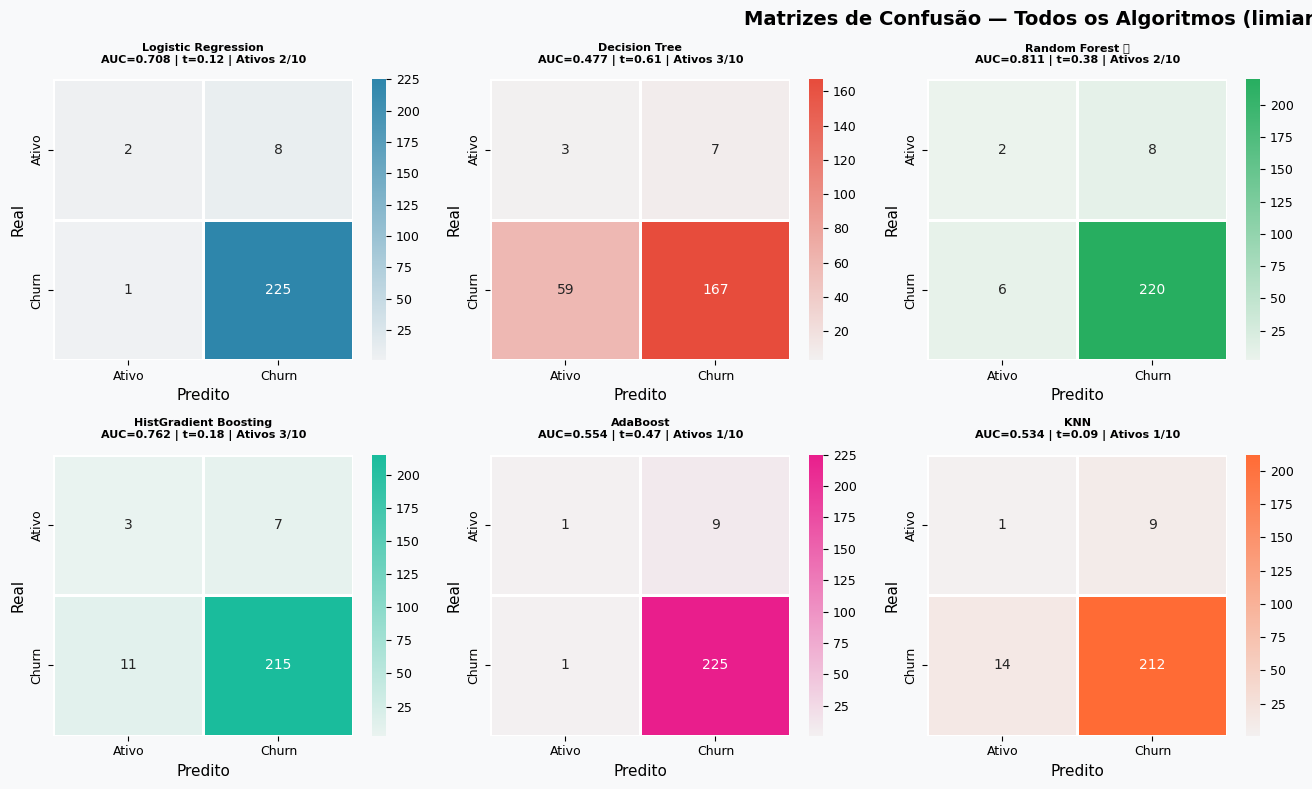
\includegraphics[width=0.95\textwidth]{USPSC-img/figuras/fig07-matrizes-confusao-a.png}
\end{center}
\begin{flushleft}
	\ABNTEXfontereduzida
	\SingleSpacing
	Fonte: elaborado pelo autor.
\end{flushleft}
\end{figure}

\begin{figure}[htbp]
\caption{Matrizes de confusão do Extra Trees, Gradient Boosting, Naive Bayes e SVM no conjunto de teste (limiar out-of-fold)}
\label{fig:matrizes-b}
\begin{center}
	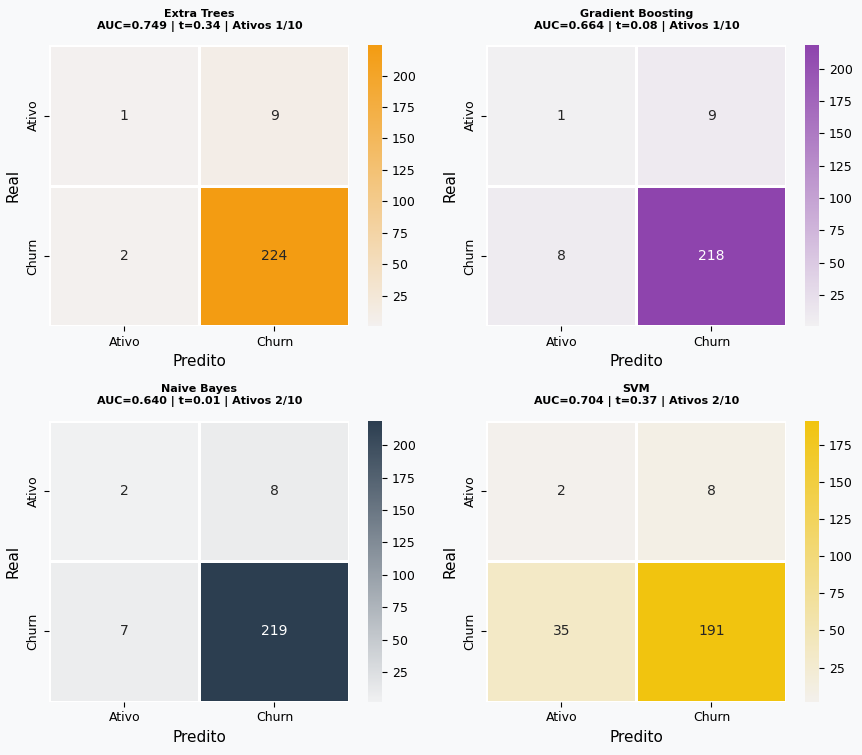
\includegraphics[width=0.95\textwidth]{USPSC-img/figuras/fig08-matrizes-confusao-b.png}
\end{center}
\begin{flushleft}
	\ABNTEXfontereduzida
	\SingleSpacing
	Fonte: elaborado pelo autor.
\end{flushleft}
\end{figure}

A Curva Precision-Recall (Figura \ref{fig:curva-pr}) corrobora a qualidade preditiva do modelo, análise especialmente apropriada em desbalanceamento severo \cite{saito2015}. A Average Precision (AP) para a classe Churn é de 0,9905, valor que deve ser lido contra a linha de base de 0,958 correspondente à prevalência dessa classe no conjunto de teste. A informação útil dessa métrica está, portanto, na comparação entre modelos, e não em sua magnitude absoluta, que é estruturalmente alta em qualquer classificador sob esse grau de desbalanceamento. Para a classe Ativo, minoritária, a AP situa-se em 0,1494, aproximadamente 3,5 vezes o baseline de um classificador aleatório (0,042), desempenho superior ao acaso, mas limitado pela escassez de exemplos positivos, apenas dez instâncias no conjunto de teste. Os valores correspondentes nos dois modelos concorrentes são de 0,2559 no HistGradient Boosting e 0,1749 na Regressão Logística, divergência analisada na Seção \ref{sec:benchmark}.

\begin{figure}[htbp]
\caption{Critério de escolha do ponto de corte em função do limiar (Random Forest)}
\label{fig:limiar-corte}
\begin{center}
	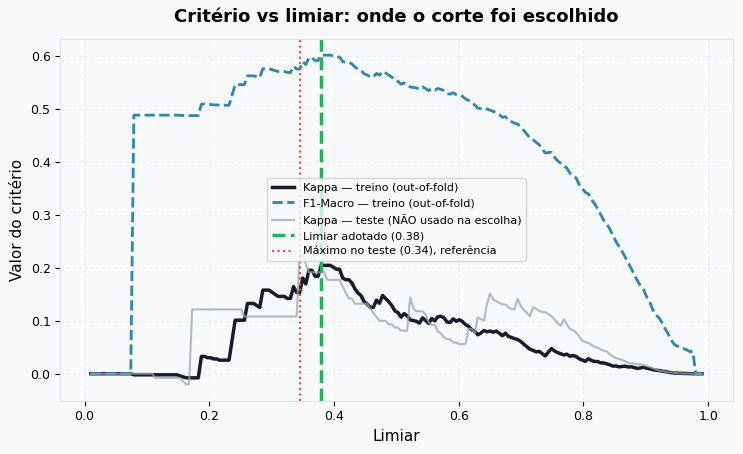
\includegraphics[width=0.9\textwidth]{USPSC-img/figuras/fig09-limiar-corte.png}
\end{center}
\begin{flushleft}
	\ABNTEXfontereduzida
	\SingleSpacing
	Fonte: elaborado pelo autor.
\end{flushleft}
\end{figure}

\begin{figure}[htbp]
\caption{Curva Precision-Recall por classe, independente do limiar (Random Forest)}
\label{fig:curva-pr}
\begin{center}
	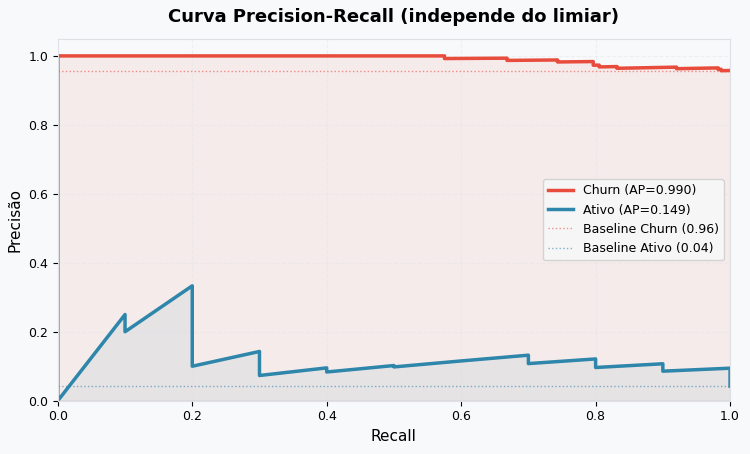
\includegraphics[width=0.9\textwidth]{USPSC-img/figuras/fig10-curva-precision-recall.png}
\end{center}
\begin{flushleft}
	\ABNTEXfontereduzida
	\SingleSpacing
	Fonte: elaborado pelo autor.
\end{flushleft}
\end{figure}

\FloatBarrier
\section{Validação da Representatividade do Balanceamento} \label{sec:representatividade}

A fim de verificar se o subconjunto da classe Churn retido no treino após o undersampling aleatório preserva a distribuição estatística da classe original \cite{he2009}, foram aplicados dois testes complementares: o Population Stability Index (PSI) e o teste de Kolmogorov-Smirnov (KS). A comparação contrapõe as 1.128 observações da classe Churn completa às 120 efetivamente utilizadas no treino após o undersampling na razão 3:1, correspondentes a uma taxa de retenção de 10,6\%. A Tabela \ref{tab:psi-ks} apresenta os resultados para as nove features numéricas.

\begin{table}[htbp]
\ABNTEXfontereduzida
\SingleSpacing
\caption{Validação de representatividade via PSI e KS-test (features numéricas)}
\label{tab:psi-ks}
\centering
\scriptsize
\setlength{\tabcolsep}{4pt}
\begin{tabular}{@{}lcrrrrrl@{}}
\hline
\textbf{Feature} & \textbf{Tipo} & \shortstack[r]{\textbf{N}\\\textbf{Completo}} & \shortstack[r]{\textbf{N}\\\textbf{Retido}} & \textbf{PSI} & \textbf{KS} & \textbf{p-valor} & \textbf{Status} \\
\hline
recency\_days       & Contínua & 1.128 & 120 & 0,0375 & 0,0574 & 0,845 & Representativa \\
frequency           & Discreta & 1.128 & 120 & 0,0039 & 0,0041 & 1,000 & Representativa \\
monetary            & Contínua & 1.128 & 120 & 0,0209 & 0,0418 & 0,987 & Representativa \\
avg\_ticket         & Contínua & 1.128 & 120 & 0,0265 & 0,0473 & 0,958 & Representativa \\
avg\_delivery\_days & Contínua & 1.128 & 120 & 0,0340 & 0,0537 & 0,896 & Representativa \\
avg\_review\_score  & Contínua & 1.128 & 120 & 0,0103 & 0,0305 & 1,000 & Representativa \\
avg\_installments   & Contínua & 1.128 & 120 & 0,1293 & 0,1035 & 0,182 & Atenção \\
avg\_freight        & Contínua & 1.128 & 120 & 0,0602 & 0,0812 & 0,448 & Representativa \\
n\_categories       & Discreta & 1.128 & 120 & 0,0022 & 0,0101 & 1,000 & Representativa \\
\hline
\end{tabular}
\begin{flushleft}
	\ABNTEXfontereduzida
	\SingleSpacing
	Fonte: elaborado pelo autor.
\end{flushleft}
\end{table}

Oito das nove features apresentaram PSI inferior a 0,10, limiar de instabilidade convencionalmente adotado, com p-valores do teste KS superiores a 0,44, indicando ausência de diferença estatisticamente significativa entre as distribuições. A única exceção é a variável avg\_installments, cujo PSI de 0,1293 situa-se na faixa de atenção, ainda que o teste KS não rejeite a hipótese de igualdade das distribuições (p = 0,182). Nenhuma feature foi classificada como distorcida.

Esses resultados são consistentes com a preservação da distribuição da classe Churn no subconjunto retido. O peso da conclusão recai sobre o PSI: oito das nove features situam-se abaixo de 0,10 e a nona, avg\_installments, permanece na faixa de atenção, sem que nenhuma variável alcance a faixa de distorção. O teste de Kolmogorov-Smirnov entra como verificação complementar, cabendo registrar que a não rejeição da hipótese de igualdade não equivale a demonstrá-la: com 120 observações retidas contra 1.128, a potência do teste é limitada, e diferenças de magnitude moderada não seriam necessariamente detectadas. Tomados em conjunto, os dois indicadores sustentam que o conjunto de treino foi construído sobre uma amostra do Churn real, e não sobre uma versão sistematicamente distorcida da classe majoritária, com desvio restrito a uma única variável de importância intermediária no modelo.

Registra-se que essa verificação alcança o undersampling da classe majoritária. A expansão sintética da classe Ativo, responsável por dois terços das instâncias minoritárias do conjunto de treino, não é objeto do mesmo teste: com quarenta observações originais, os testes empregados teriam potência insuficiente para distinguir a distribuição sintética da original. Sua adequação é discutida qualitativamente no Quadro \ref{qua:estrategias-balanceamento} e na Seção \ref{subsec:clientes-informativos}, e a validação quantitativa da perturbação gaussiana permanece entre os trabalhos futuros.

\subsection{Discussão: representatividade e clientes informativos} \label{subsec:clientes-informativos}

A validação por PSI e KS-test atesta que o undersampling aleatório preserva a distribuição estatística marginal das features. Cabe, contudo, uma reflexão metodológica complementar: a estratégia de seleção aleatória trata todas as observações da classe majoritária como igualmente informativas, hipótese que nem sempre se sustenta. A literatura de aprendizado sensível a instâncias distingue observações seguras, que representam de forma confiável a região central da distribuição, de observações redundantes ou ruidosas, cuja remoção não compromete, e pode até favorecer, a capacidade discriminativa do modelo \cite{kubat1997}.

No contexto deste trabalho, essa perspectiva é particularmente relevante para a classe minoritária, composta por aproximadamente 50 clientes Ativos. Por se tratar de uma amostra reduzida, cada observação da classe Ativo representa parcela expressiva da informação disponível sobre o comportamento de recompra, razão pela qual a perturbação gaussiana adotada no oversampling preserva integralmente as observações originais, em vez de substituí-las por instâncias interpoladas.

Uma extensão natural seria substituir o undersampling aleatório da classe Churn por uma seleção orientada por informatividade, como o one-sided selection \cite{kubat1997}, que remove observações redundantes e ruidosas da classe majoritária, retendo preferencialmente as mais confiáveis. Dado que o undersampling aleatório demonstrou representatividade estatística em oito das nove features analisadas, conforme a Seção \ref{sec:representatividade}, é razoável esperar que o ganho marginal dessa abordagem seja limitado neste dataset específico, ainda que essa hipótese não tenha sido testada empiricamente. A seleção orientada por informatividade permanece, assim, como direção promissora para bases de maior volume, e é registrada entre os trabalhos futuros.

\FloatBarrier
\section{Interpretabilidade: Importância das Features e SHAP} \label{sec:interpretabilidade}

A análise de importância de features via impureza de Gini \cite{breiman2001} revelou que a frequência de compras é, com folga, a variável mais determinante para a predição do churn, respondendo por 23,19\% da importância total do modelo (Tabela \ref{tab:importancia-gini}). As cinco features mais relevantes, frequency (23,19\%), recency\_days (12,19\%), n\_categories (11,88\%), avg\_installments (7,84\%) e avg\_delivery\_days (7,41\%), respondem conjuntamente por 62,52\% da importância total. Destaca-se que recency\_days e n\_categories encontram-se em empate técnico: a diferença de importância entre ambas é de aproximadamente 0,3 ponto percentual, de modo que a ordenação exata entre a segunda e a terceira posições é sensível a variações de implementação e de versão de biblioteca \cite{pedregosa2011}, embora a composição do trio dominante, frequência, recência e diversidade de categorias, permaneça estável entre execuções.

\begin{table}[htbp]
\ABNTEXfontereduzida
\SingleSpacing
\caption{Importância das cinco principais features do modelo Random Forest (Gini)}
\label{tab:importancia-gini}
\centering
\begin{tabular}{@{}cl r >{\raggedright\arraybackslash}p{7.6cm}@{}}
\hline
\textbf{Pos.} & \textbf{Feature} & \textbf{Importância} & \textbf{Insight Estratégico} \\
\hline
1\textsuperscript{a} & frequency & 23,19\% & Principal driver de recompra: clientes que compram mais vezes apresentam menor propensão ao churn \\
2\textsuperscript{a} & recency\_days & 12,19\% & Recência elevada é forte sinal de inatividade iminente; empate técnico com n\_categories \\
3\textsuperscript{a} & n\_categories & 11,88\% & Diversidade de categorias como proxy de engajamento; empate técnico com recency\_days \\
4\textsuperscript{a} & avg\_installments & 7,84\% & Uso de parcelamento em mais vezes associa-se a maior risco, sugerindo compras pontuais em vez de relacionamento recorrente \\
5\textsuperscript{a} & avg\_delivery\_days & 7,41\% & Tempo de entrega como fator de experiência que influencia a decisão de retorno \\
\hline
\end{tabular}
\begin{flushleft}
	\ABNTEXfontereduzida
	\SingleSpacing
	Fonte: elaborado pelo autor.

	\textit{Nota: recency\_days e n\_categories apresentam importâncias em empate técnico, com diferença de aproximadamente 0,3 ponto percentual. Dada essa proximidade, a ordenação exata entre a 2\textsuperscript{a} e a 3\textsuperscript{a} posições não deve ser interpretada como hierarquia estabelecida, ainda que a composição do trio dominante permaneça consistente. As importâncias são apresentadas com duas casas decimais; o total de 62,52\% reportado no texto é calculado sobre os valores sem arredondamento, cuja soma é 0,625163.}
\end{flushleft}
\end{table}

O resultado para n\_categories (número de categorias distintas adquiridas) merece destaque especial: sua presença consistente entre os três principais drivers preditivos, em empate técnico com a recência, sugere que a diversidade de categorias de compra é um forte indicador de engajamento com a plataforma. A Figura \ref{fig:importancia-gini} apresenta a importância relativa de todas as variáveis, evidenciando o domínio de frequency e a proximidade entre recency\_days e n\_categories, e a Figura \ref{fig:top5-gini} destaca o recorte das cinco primeiras posições. Esse achado reforça a relevância da diversidade de compras como indicador de engajamento, aspecto pouco explorado na literatura de churn aplicada ao Olist. Clientes que compram em múltiplas categorias tendem a apresentar maior propensão ao retorno, o que representa insumo relevante para estratégias de cross-selling visando à retenção \cite{kotler2016}.

\begin{figure}[htbp]
\caption{Importância das features por impureza de Gini (Random Forest)}
\label{fig:importancia-gini}
\begin{center}
	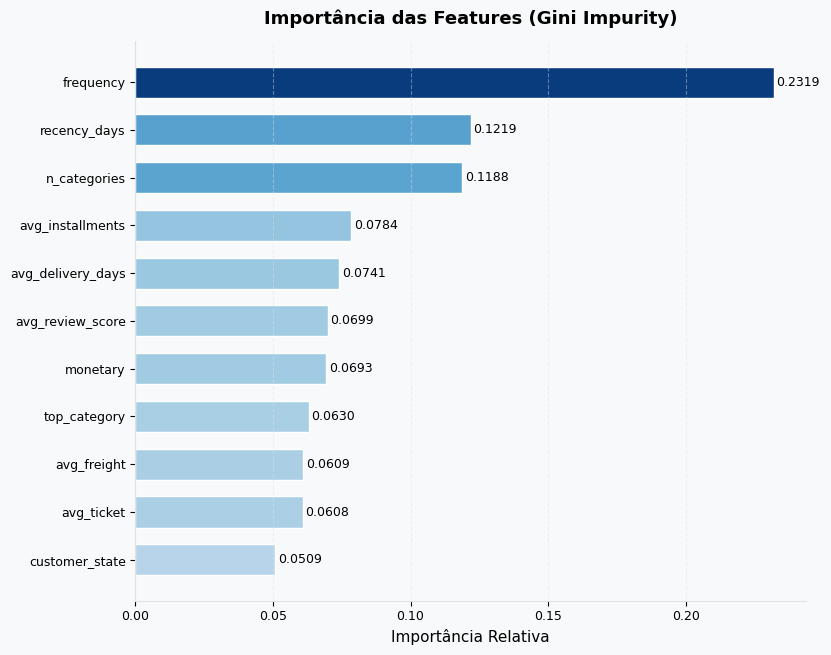
\includegraphics[width=0.9\textwidth]{USPSC-img/figuras/fig11-importancia-gini.png}
\end{center}
\begin{flushleft}
	\ABNTEXfontereduzida
	\SingleSpacing
	Fonte: elaborado pelo autor.
\end{flushleft}
\end{figure}

\begin{figure}[htbp]
\caption{Top-5 Features por impureza de Gini (Random Forest)}
\label{fig:top5-gini}
\begin{center}
	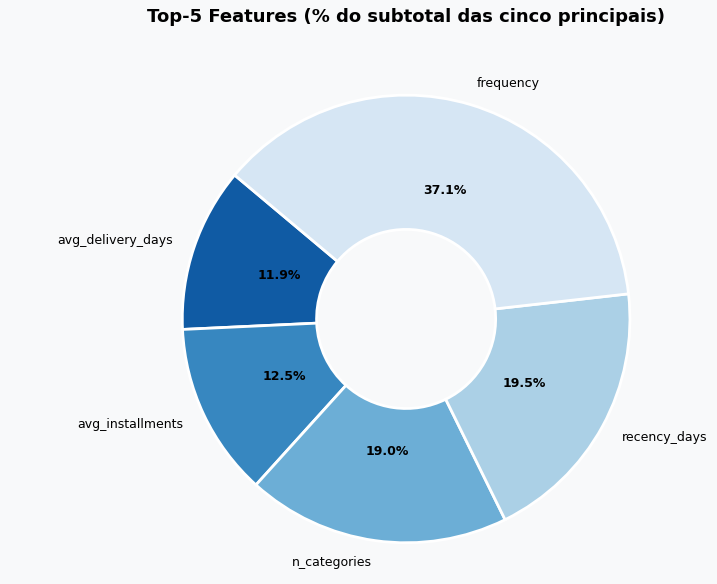
\includegraphics[width=0.85\textwidth]{USPSC-img/figuras/fig12-top5-gini.png}
\end{center}
\begin{flushleft}
	\ABNTEXfontereduzida
	\SingleSpacing
	Fonte: elaborado pelo autor.
\end{flushleft}
\end{figure}

A análise SHAP via TreeExplainer \cite{lundberg2020} enriquece o ranking de Gini ao revelar as direções dos efeitos (Figura \ref{fig:shap-beeswarm}). A Figura \ref{fig:shap-importancia} apresenta a importância média absoluta dos valores SHAP, cuja ordenação pode ser confrontada diretamente com a da Figura \ref{fig:importancia-gini}. A concordância entre os dois métodos é elevada: as quatro features mais relevantes ocupam posições idênticas em ambos os rankings, com divergência superior a uma posição em apenas duas das onze variáveis. Cabe registrar, contudo, que essa concordância não constitui validação independente da hierarquia de importância. A importância por impureza de Gini quantifica a redução de impureza produzida por cada variável nas árvores ajustadas, e o TreeSHAP percorre exatamente essas mesmas árvores para decompor as predições: ambos os estimadores derivam da mesma estrutura de modelo, de modo que sua concordância é esperada por construção. A evidência de estabilidade adotada neste trabalho é de outra natureza e apresenta-se a seguir. O valor base do modelo, $\mathbb{E}[f(x)] = 0{,}504$, reflete o balanceamento aplicado ao conjunto de treino, conforme discutido na Seção \ref{sec:limiar}.

\begin{figure}[htbp]
\caption{Importância média \shapabs{} das features (Random Forest)}
\label{fig:shap-importancia}
\begin{center}
	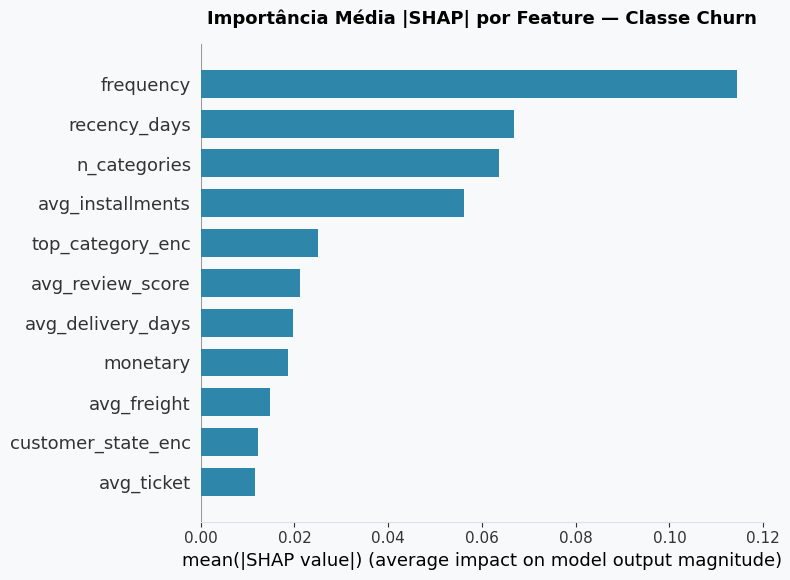
\includegraphics[width=0.9\textwidth]{USPSC-img/figuras/fig13-shap-importancia-media.png}
\end{center}
\begin{flushleft}
	\ABNTEXfontereduzida
	\SingleSpacing
	Fonte: elaborado pelo autor.
\end{flushleft}
\end{figure}

Para verificar a estabilidade da ordenação por critério independente do estimador, o modelo foi reajustado em trinta partições estratificadas independentes, registrando-se a posição de cada feature no ranking de importância por Gini em cada uma delas. A variável frequency ocupou a primeira posição nas trinta partições, sem exceção. A variável n\_categories permaneceu entre as três primeiras em 29 das trinta, com posições variando entre a segunda e a quarta, e recency\_days em 22 das trinta, com posições entre a segunda e a quinta. A variável seguinte em estabilidade, monetary, figurou entre as três primeiras em apenas quatro partições, o que delimita com clareza o trio dominante. Esse resultado sustenta a afirmação de estabilidade da hierarquia entre partições e, adicionalmente, confirma o empate técnico entre recency\_days e n\_categories registrado na Tabela \ref{tab:importancia-gini}: embora a recência esteja 0,3 ponto percentual à frente na partição de referência, a diversidade de categorias apresenta posição média superior no conjunto das trinta partições (2,30 contra 3,17).

Registra-se, por completude, que um terceiro estimador de importância, a permutação de features calculada sobre o conjunto de teste, produz ordenação distinta das duas anteriores, elevando avg\_installments à primeira posição e deslocando frequency para a quarta. Esse estimador não é informativo no regime amostral deste trabalho: com dez instâncias da classe Ativo no hold-out, o desvio-padrão de cada estimativa situa-se entre 44\% e 93\% da respectiva média nas nove variáveis de média positiva, e as duas restantes apresentam média negativa, valor que não admite interpretação substantiva. A imprecisão é suficiente para dissolver a própria ordenação que o estimador produz: a primeira e a segunda colocadas, avg\_installments (0,0788 $\pm$ 0,0449) e recency\_days (0,0721 $\pm$ 0,0508), apresentam intervalos amplamente sobrepostos. A divergência observada não refuta, portanto, a ordenação por Gini, mas impede que se afirme robustez da hierarquia ao método de estimação, razão pela qual a estabilidade entre partições foi adotada como evidência.

A análise de interpretabilidade conduzida até aqui apoia-se no Random Forest, modelo de produção. Cabe verificar em que medida a hierarquia de importância obtida é propriedade dos dados ou artefato do estimador escolhido. A importância por impureza de Gini não permite essa verificação, por não estar disponível no HistGradientBoostingClassifier nem se aplicar a modelos lineares. Os valores SHAP, ao contrário, são calculáveis para os três modelos e constituem, portanto, o único terreno comum de comparação. A Tabela \ref{tab:shap-tres-modelos} apresenta a posição de cada feature no ranking por importância média absoluta e sua participação relativa no total de cada modelo, calculadas sobre o mesmo conjunto de teste.

\begin{table}[htbp]
\ABNTEXfontereduzida
\SingleSpacing
\caption{Posição e participação relativa das features no ranking por importância média \shapabs{} nos três modelos}
\label{tab:shap-tres-modelos}
\centering
\begin{tabular}{@{}lcccrrr@{}}
\hline
\textbf{Feature} & \textbf{Pos. RF} & \textbf{Pos. HistGB} & \textbf{Pos. RL} & \textbf{\% RF} & \textbf{\% HistGB} & \textbf{\% RL} \\
\hline
frequency          & 1\textsuperscript{a}  & 1\textsuperscript{a}  & 3\textsuperscript{a}  & 27,0 & 19,4 & 13,9 \\
recency\_days      & 2\textsuperscript{a}  & 2\textsuperscript{a}  & 2\textsuperscript{a}  & 15,7 & 13,4 & 19,0 \\
n\_categories      & 3\textsuperscript{a}  & 6\textsuperscript{a}  & 4\textsuperscript{a}  & 15,0 & 8,2  & 10,6 \\
avg\_installments  & 4\textsuperscript{a}  & 4\textsuperscript{a}  & 1\textsuperscript{a}  & 13,2 & 11,7 & 21,0 \\
top\_category      & 5\textsuperscript{a}  & 5\textsuperscript{a}  & 7\textsuperscript{a}  & 5,9  & 9,5  & 6,1 \\
avg\_review\_score & 6\textsuperscript{a}  & 9\textsuperscript{a}  & 8\textsuperscript{a}  & 5,0  & 4,9  & 5,8 \\
avg\_delivery\_days& 7\textsuperscript{a}  & 3\textsuperscript{a}  & 6\textsuperscript{a}  & 4,7  & 11,8 & 6,4 \\
monetary           & 8\textsuperscript{a}  & 7\textsuperscript{a}  & 9\textsuperscript{a}  & 4,4  & 6,4  & 4,7 \\
avg\_freight       & 9\textsuperscript{a}  & 11\textsuperscript{a} & 11\textsuperscript{a} & 3,5  & 4,3  & 2,5 \\
customer\_state    & 10\textsuperscript{a} & 8\textsuperscript{a}  & 10\textsuperscript{a} & 2,9  & 5,9  & 3,7 \\
avg\_ticket        & 11\textsuperscript{a} & 10\textsuperscript{a} & 5\textsuperscript{a}  & 2,7  & 4,6  & 6,4 \\
\hline
\end{tabular}
\begin{flushleft}
	\ABNTEXfontereduzida
	\SingleSpacing
	Fonte: elaborado pelo autor.

	\textit{Nota: RF designa o Random Forest, HistGB o HistGradient Boosting e RL a Regressão Logística. Os valores absolutos de \shapabs{} não são comparáveis entre modelos e por isso não são reportados: o TreeExplainer aplicado ao Random Forest devolve contribuições em espaço de probabilidade, ao passo que o HistGradient Boosting e a Regressão Logística as devolvem em log-odds. São comparáveis a posição no ranking e a participação relativa, esta definida como a importância média absoluta da feature dividida pela soma das importâncias das onze features do mesmo modelo. Para a Regressão Logística os valores foram obtidos por LinearExplainer, que sob independência de features corresponde à forma fechada apresentada na Seção \ref{sec:shap-teorico}. Conjunto de teste, n = 236.}
\end{flushleft}
\end{table}

A convergência entre os três estimadores é substancial e estatisticamente significativa: a correlação de Spearman entre os rankings é de 0,800 entre Random Forest e HistGradient Boosting (p = 0,003) e de 0,709 nos dois pares que envolvem a Regressão Logística (p = 0,015). A recência ocupa a segunda posição nos três modelos, sem exceção, o que a torna o achado mais robusto da análise de interpretabilidade. A frequência lidera nos dois modelos baseados em árvores e cai para a terceira posição no modelo linear, resultado coerente com a natureza da relação: o beeswarm plot evidencia que o efeito da frequência é essencialmente descontínuo, concentrado na diferença entre dois pedidos e mais de dois, padrão que um modelo linear captura apenas parcialmente.

Registram-se duas divergências relevantes. A primeira é a variável avg\_installments, que ocupa a primeira posição na Regressão Logística e a quarta nos dois ensembles; sua elevação também havia sido observada pela importância por permutação, o que constitui indício independente de que seu peso é subestimado pelo Gini, ainda que aquele estimador não seja informativo neste regime amostral. A segunda é avg\_delivery\_days, terceira no HistGradient Boosting e sétima no Random Forest, deslocamento que sugere sensibilidade do algoritmo de boosting a limiares do tempo de entrega não capturados pelo ensemble por bagging. A variável n\_categories, terceira no Random Forest e quarta na Regressão Logística, cai para a sexta posição no HistGradient Boosting, de modo que a composição do trio dominante identificada nesta seção é confirmada por dois dos três estimadores, e não pelos três.

O beeswarm plot evidencia que valores baixos de frequency (poucos pedidos) aumentam significativamente a probabilidade predita de churn, enquanto valores altos a reduzem, relação capturada por uma correlação de $-0{,}862$ entre o valor da feature e sua contribuição SHAP. Para n\_categories, o padrão é análogo (correlação de $-0{,}648$): clientes com maior diversidade de categorias apresentam contribuições SHAP negativas para o churn, ou seja, a diversidade reduz o risco predito. Para recency\_days, a direção é a esperada e a associação é a mais forte entre as três (correlação de $+0{,}895$): maior recência eleva o risco de churn. Os dependence plots e os waterfall plots de instâncias representativas, apresentados ao final desta seção, detalham respectivamente os limiares não lineares dessas relações e a decomposição individual da predição para clientes típicos de cada classe.

Registra-se, como divergência pontual entre os métodos, que a variável top\_category ocupa a quinta posição no ranking SHAP, três posições acima do observado pela impureza de Gini. Esse deslocamento sugere que a categoria dominante de compra exerce efeito direcional mais relevante do que a redução de impureza isoladamente permite inferir, achado consistente com a limitação conhecida da importância por Gini em variáveis categóricas de cardinalidade elevada.

\begin{figure}[htbp]
\caption{Valores SHAP (beeswarm) das features no conjunto de teste}
\label{fig:shap-beeswarm}
\begin{center}
	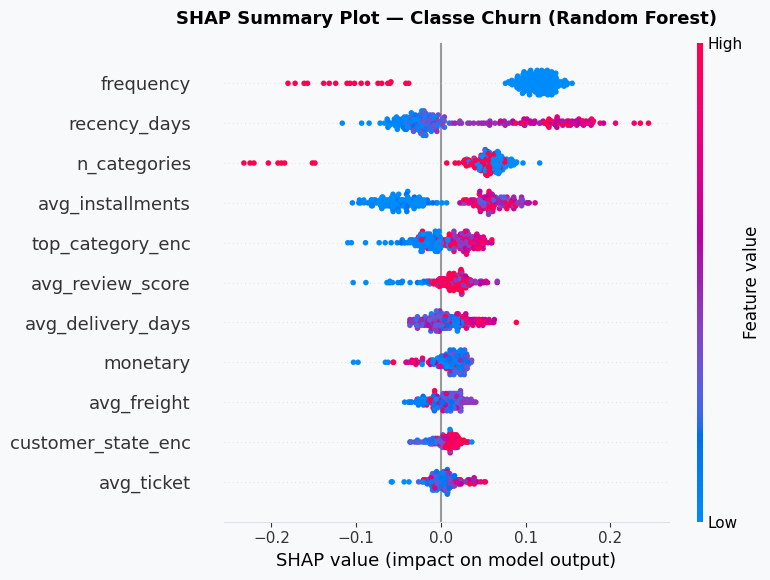
\includegraphics[width=0.9\textwidth]{USPSC-img/figuras/fig14-shap-beeswarm.png}
\end{center}
\begin{flushleft}
	\ABNTEXfontereduzida
	\SingleSpacing
	Fonte: elaborado pelo autor.
\end{flushleft}
\end{figure}

\subsection{Perfil do cliente que retorna: leitura sob a ótica da retenção} \label{subsec:perfil-retorna}

Embora a variável-alvo seja formalmente o churn, os valores SHAP permitem inverter a leitura e caracterizar diretamente o perfil do cliente que volta a comprar, objetivo de maior valor acionável para a organização. As contribuições SHAP que reduzem a probabilidade de churn correspondem, por complementaridade, aos atributos associados à retenção. Sob essa ótica, o cliente com maior propensão a retornar à plataforma apresenta o seguinte perfil: (i) realiza compras com maior frequência (2,56 pedidos em média, contra 2,08 entre os clientes Churn, conforme a Seção \ref{sec:eda}); (ii) mantém recência baixa, com intervalos curtos entre transações; e (iii) compra em mais categorias distintas (n\_categories elevado), indicando exploração ampla do catálogo. Em contraste, o uso de parcelamento em mais vezes (avg\_installments elevado) associa-se a maior risco de churn, possivelmente por sinalizar compras pontuais de maior ticket em vez de um relacionamento recorrente com a loja. Cabe observar que essa última variável é a que ocupa a primeira posição no ranking SHAP da Regressão Logística (Tabela \ref{tab:shap-tres-modelos}), o que sugere que seu efeito seja predominantemente monotônico e, por isso, mais bem capturado por um modelo linear.

Esse achado tem implicação estratégica direta: a diversidade de categorias, um dos três principais drivers do modelo, sugere que estimular o cliente a explorar novas categorias, via recomendação e cross-selling, é mecanismo promissor para elevar a probabilidade de retorno \cite{kotler2016}. A análise exploratória (Seção \ref{sec:eda}) corrobora esse perfil ao mostrar que clientes Ativos apresentam maior valor monetário acumulado (R\$ 372,25 contra R\$ 299,12) e compram em categorias mais variadas (1,80 contra 1,54 categorias, em média) que os clientes Churn. Cabe observar que o valor monetário acumulado, embora discrimine as classes na análise exploratória, ocupa apenas a sétima posição na importância por impureza de Gini, o que sugere que seu poder preditivo é em parte absorvido pela frequência de compras, com a qual mantém dependência direta.

Registra-se, como ressalva metodológica, que a classe Ativo conta com aproximadamente 50 clientes na base completa, de modo que o perfil de retenção descrito, ainda que consistente entre a análise exploratória, a importância por Gini estimada em trinta partições e os valores SHAP dos três modelos, deve ser interpretado como hipótese robusta a ser confirmada em bases de maior volume.

Todos os valores das figuras abaixo referem-se ao modelo Random Forest adotado como modelo de produção, calculados sobre o conjunto de teste. Os dependence plots das Figuras \ref{fig:dep-frequency}, \ref{fig:dep-recency} e \ref{fig:dep-ncategories} evidenciam que as relações capturadas pelo modelo não são lineares. Para frequency, as contribuições concentram-se em dois agrupamentos disjuntos: clientes com dois pedidos recebem contribuição positiva para o churn, entre 0,08 e 0,15, e clientes com três ou mais pedidos recebem contribuição negativa, o que caracteriza um limiar de decisão e não uma tendência gradual. Para recency\_days a relação é monotônica crescente e aproximadamente sigmóide, com a transição de contribuição negativa para positiva ocorrendo em torno da média da distribuição padronizada. Para n\_categories o padrão repete a descontinuidade observada em frequency, com separação nítida entre clientes de uma ou duas categorias e clientes de três ou mais. Essa descontinuidade é a razão estrutural pela qual a frequência perde posições no ranking SHAP da Regressão Logística (Tabela \ref{tab:shap-tres-modelos}): um modelo linear não representa limiares dessa natureza.

\begin{figure}[H]
\caption{Dependence plots da feature frequency no SHAP (Random Forest)}
\label{fig:dep-frequency}
\begin{center}
	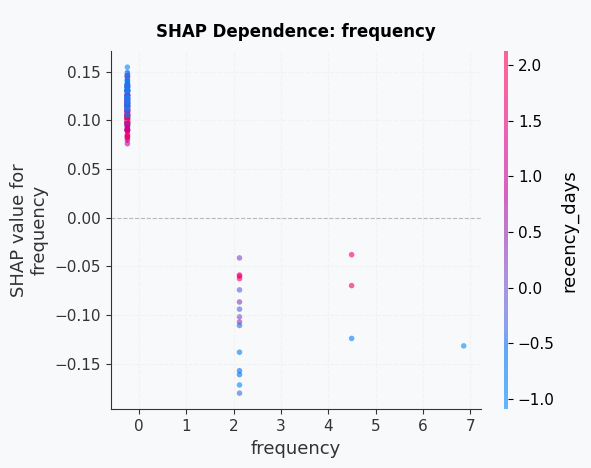
\includegraphics[width=0.80\textwidth]{USPSC-img/figuras/fig15-shap-dependence-frequency.png}
\end{center}
\begin{flushleft}
	\ABNTEXfontereduzida
	\SingleSpacing
	Fonte: elaborado pelo autor.
\end{flushleft}
\end{figure}

\begin{figure}[H]
\caption{Dependence plots da feature recency\_days no SHAP (Random Forest)}
\label{fig:dep-recency}
\begin{center}
	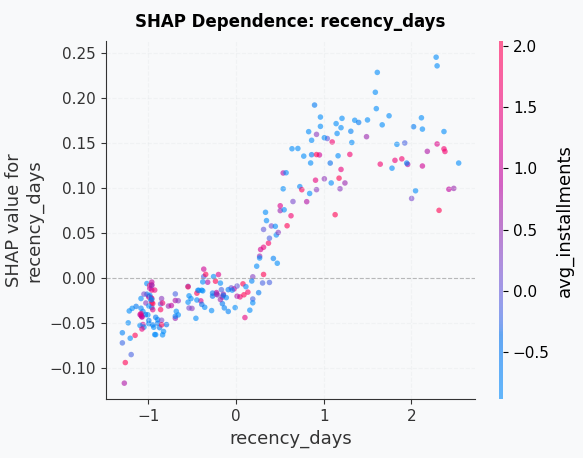
\includegraphics[width=0.85\textwidth]{USPSC-img/figuras/fig16-shap-dependence-recency.png}
\end{center}
\begin{flushleft}
	\ABNTEXfontereduzida
	\SingleSpacing
	Fonte: elaborado pelo autor.
\end{flushleft}
\end{figure}

\begin{figure}[H]
\caption{Dependence plots da feature n\_categories no SHAP (Random Forest)}
\label{fig:dep-ncategories}
\begin{center}
	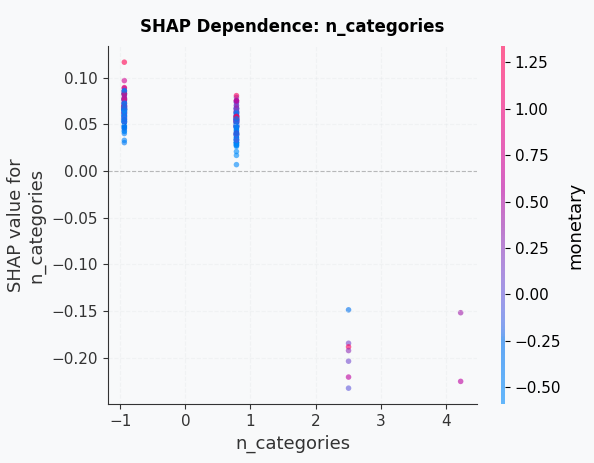
\includegraphics[width=0.85\textwidth]{USPSC-img/figuras/fig17-shap-dependence-ncategories.png}
\end{center}
\begin{flushleft}
	\ABNTEXfontereduzida
	\SingleSpacing
	Fonte: elaborado pelo autor.
\end{flushleft}
\end{figure}

As Figuras \ref{fig:waterfall-ativo} e \ref{fig:waterfall-churn} decompõem a predição individual dos clientes mais próximos do centroide de cada classe no espaço de features padronizado. Ambas partem do mesmo valor base, $\mathbb{E}[f(x)] = 0{,}504$, que reflete o balanceamento aplicado ao conjunto de treino conforme a Seção \ref{sec:limiar}.

O cliente representativo da classe Churn (Figura \ref{fig:waterfall-churn}) recebe $f(x) = 0{,}841$, valor consistente com sua classe real. A decomposição atribui o deslocamento principalmente à frequência ($+0{,}12$), à diversidade de categorias ($+0{,}08$) e ao parcelamento médio ($+0{,}07$), reproduzindo em nível individual a hierarquia agregada da Figura \ref{fig:shap-importancia}.

O cliente representativo da classe Ativo (Figura \ref{fig:waterfall-ativo}) recebe $f(x) = 0{,}613$, valor acima do limiar de 0,38 e que, portanto, o classifica incorretamente como Churn. Longe de invalidar a ilustração, esse resultado a torna mais informativa: o cliente mais próximo do centroide da classe Ativo apresenta frequência e diversidade de categorias abaixo da média da base, atributos que o modelo associa ao abandono, e as contribuições que o afastam do churn, o parcelamento médio ($-0{,}06$) e a recência ($-0{,}03$), são insuficientes para compensá-los. A figura expõe, em um caso concreto, a razão do Recall de 0,20 na classe Ativo reportado na Tabela \ref{tab:benchmark}: o perfil médio do cliente que retorna não é suficientemente distinto do perfil do cliente que abandona, limitação devida ao tamanho reduzido da classe minoritária e não à especificação do modelo. Esse é também o fundamento do critério de seleção adotado na Seção \ref{sec:benchmark}: uma vez que a decisão binária no limiar é estruturalmente limitada por esse regime amostral, o valor operacional do modelo reside na ordenação que ele produz, e não na classificação que dela resulta.

\begin{figure}[htbp]
\caption{Decomposição SHAP da predição para o cliente mais próximo do centroide da classe Ativo}
\label{fig:waterfall-ativo}
\begin{center}
	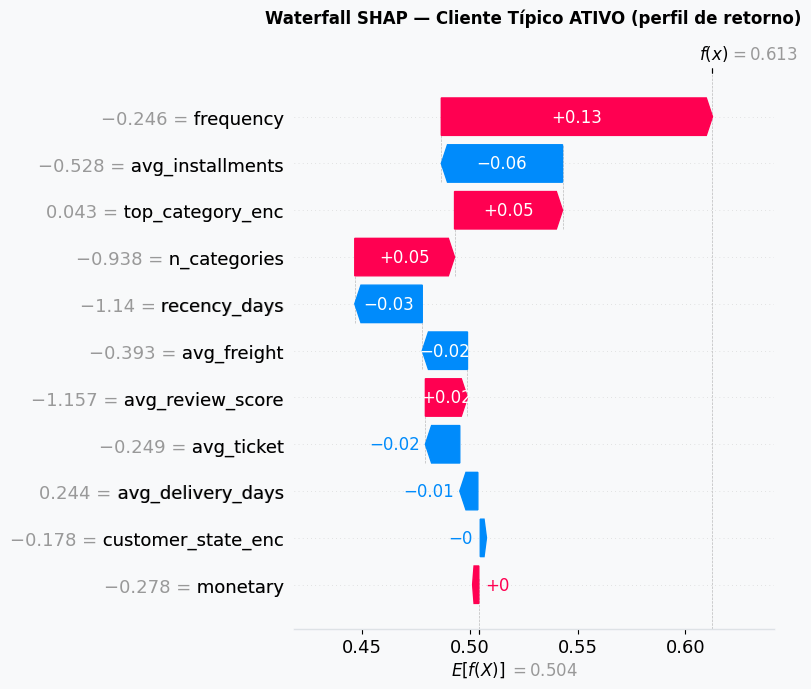
\includegraphics[width=0.9\textwidth]{USPSC-img/figuras/fig18-shap-waterfall-ativo.png}
\end{center}
\begin{flushleft}
	\ABNTEXfontereduzida
	\SingleSpacing
	Fonte: elaborado pelo autor.
\end{flushleft}
\end{figure}

\begin{figure}[htbp]
\caption{Decomposição SHAP da predição para o cliente mais próximo do centroide da classe Churn}
\label{fig:waterfall-churn}
\begin{center}
	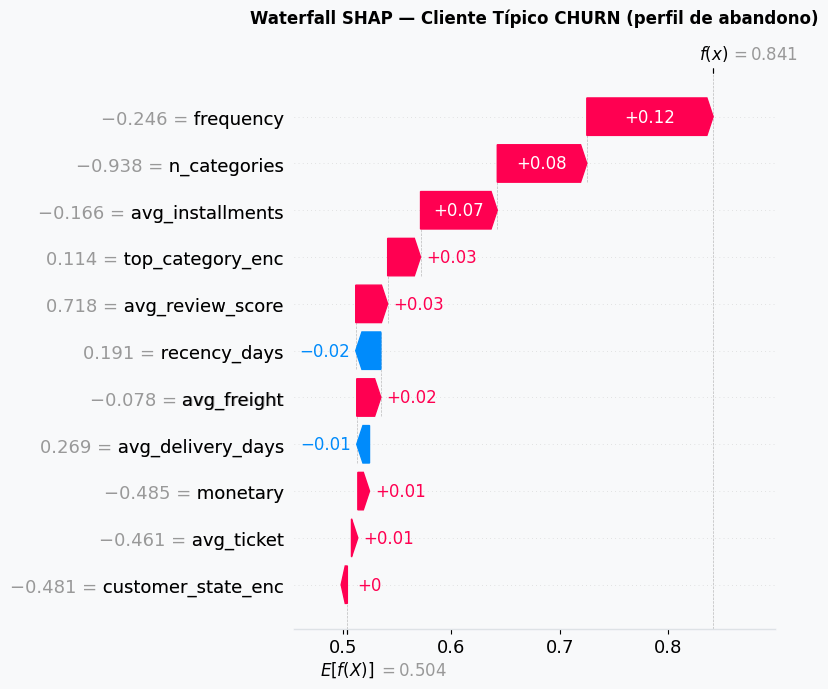
\includegraphics[width=0.9\textwidth]{USPSC-img/figuras/fig19-shap-waterfall-churn.png}
\end{center}
\begin{flushleft}
	\ABNTEXfontereduzida
	\SingleSpacing
	Fonte: elaborado pelo autor.
\end{flushleft}
\end{figure}

\FloatBarrier
\section{Segmentação de Risco e Recomendações de Negócio} \label{sec:segmentacao}

Aplicado o modelo Random Forest à base completa de 1.178 clientes, cada cliente recebeu um score de probabilidade de churn, utilizado para classificação em quatro segmentos de risco \cite{kotler2016}. Os limiares de 25\%, 50\% e 75\% que delimitam os segmentos são cortes nominais da escala de probabilidade, adotados por interpretabilidade e não otimizados sobre os dados; sua adequação é aferida a posteriori pela taxa de churn observada em cada faixa. A Figura \ref{fig:distribuicao-scores} apresenta a distribuição desses scores nos três modelos de melhor desempenho, com os limiares que delimitam os quatro segmentos, e a Tabela \ref{tab:segmentacao} detalha a distribuição e o perfil médio de cada segmento sob o modelo de produção.

\begin{figure}[htbp]
\caption{Distribuição dos scores de probabilidade de churn e limiares de segmentação nos três modelos}
\label{fig:distribuicao-scores}
\begin{center}
	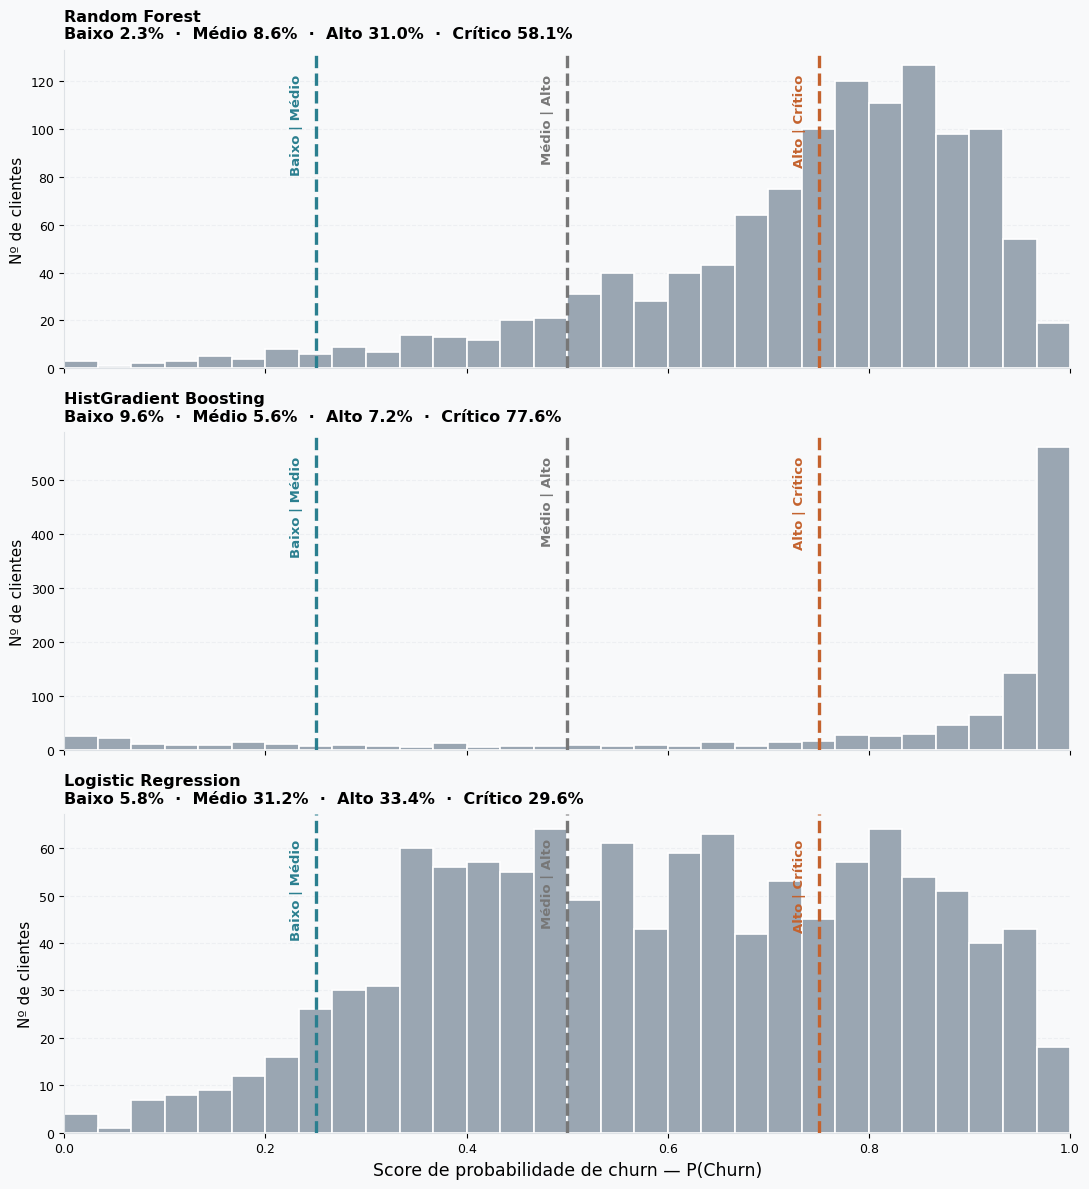
\includegraphics[width=0.95\textwidth]{USPSC-img/figuras/fig20-distribuicao-scores.png}
\end{center}
\begin{flushleft}
	\ABNTEXfontereduzida
	\SingleSpacing
	Fonte: elaborado pelo autor.

	\textit{Nota: os três painéis aplicam os mesmos cortes nominais de 25\%, 50\% e 75\%, que delimitam os segmentos de risco e não correspondem ao limiar de classificação de cada modelo (0,38 no Random Forest, 0,18 no HistGradient Boosting e 0,12 na Regressão Logística, conforme a Tabela \ref{tab:benchmark}). Os cortes de segmentação são uma escolha de negócio, aferida a posteriori pela taxa de churn observada em cada faixa; o limiar de classificação é parâmetro da regra de decisão binária, derivado das probabilidades out-of-fold conforme a Seção \ref{sec:protocolo}. Escopo: base completa de 1.178 clientes.}
\end{flushleft}
\end{figure}

\begin{table}[htbp]
\ABNTEXfontereduzida
\SingleSpacing
\caption{Segmentação de risco de churn e ações recomendadas por segmento}
\label{tab:segmentacao}
\centering
\setlength{\tabcolsep}{4pt}
\begin{tabular}{@{}l c r r >{\raggedright\arraybackslash}p{4.7cm}@{}}
\hline
\textbf{Segmento} & \textbf{Critério} & \textbf{Clientes} & \shortstack[r]{\textbf{Recência}\\\textbf{Média}} & \textbf{Ação Recomendada} \\
\hline
Crítico & $P > 75\%$              & 685 (58,1\%) & 147,95 dias & Ação urgente: cupons e contato direto \\
Alto    & $50\% < P \leq 75\%$    & 365 (31,0\%) & 95,78 dias  & Ofertas e descontos personalizados \\
Médio   & $25\% < P \leq 50\%$    & 101 (8,6\%)  & 80,72 dias  & Campanhas de reengajamento leve \\
Baixo   & $P \leq 25\%$           & 27 (2,3\%)   & 72,52 dias  & Cross-sell e manutenção de engajamento \\
\hline
\end{tabular}
\begin{flushleft}
	\ABNTEXfontereduzida
	\SingleSpacing
	Fonte: elaborado pelo autor.
\end{flushleft}
\end{table}

A validade da segmentação é aferida pela taxa de churn efetivamente observada em cada faixa, isto é, pelo próprio rótulo que o modelo busca prever, e não por variáveis que integram seu conjunto de entrada. Cabe, antes, uma delimitação de escopo: a Tabela \ref{tab:segmentacao} descreve a base completa de 1.178 clientes, que inclui as observações utilizadas no ajuste do modelo, de modo que suas contagens refletem, em parte, o comportamento do classificador sobre dados já vistos. Sobre essa base, a taxa cresce de forma estritamente monotônica ao longo dos segmentos: 22,2\% no Baixo, 79,2\% no Médio, 98,1\% no Alto e 99,9\% no Crítico, com amplitude de 77,6 pontos percentuais entre os extremos.

A leitura com valor preditivo, contudo, é restrita ao conjunto de teste, cujos 236 clientes não participaram do ajuste. Nele, a progressão mantém-se na mesma direção (75,0\% no Baixo e 99,3\% no Crítico), com inversão entre as faixas Médio e Alto atribuível ao reduzido número de observações por segmento. Os dez clientes ativos do conjunto de teste distribuem-se em um no Baixo, um no Médio, sete no Alto e um no Crítico. O resultado operacionalmente relevante está, portanto, na exclusão da faixa Crítico: fora dela permanecem nove dos dez clientes Ativos, em 92 das 236 observações (39,0\%), o que corresponde a um lift de 2,31 vezes sobre a proporção de Ativos no conjunto de teste (4,2\%). A mesma métrica calculada sobre a base completa resulta em 2,34 vezes (49 dos 50 Ativos em 41,9\% das observações), estabilidade que indica não haver, nesse recorte, ganho atribuível à memorização das observações de treino.

Registra-se, por transparência, que o recorte alternativo composto pelas duas faixas de menor risco não apresenta a mesma estabilidade: na base completa ele reúne 42 dos 50 clientes Ativos em 10,9\% das observações, lift de 7,73 vezes, mas no conjunto de teste reúne apenas dois dos dez em 8,1\%, lift de 2,48 vezes. A diferença decorre de os quarenta clientes ativos presentes no conjunto de treino situarem-se integralmente nessas duas faixas. Verifica-se, assim, que a estratificação separa risco fora da amostra, com magnitude da ordem de duas vezes, magnitude que deve ser lida com cautela em razão do número reduzido de clientes Ativos no conjunto de teste.

Com base nos scores de risco, propõem-se ações diferenciadas de retenção: clientes no segmento Baixo devem ser priorizados para cross-sell; no Médio, são candidatos a campanhas de reengajamento leve, como newsletters; o segmento Alto requer abordagem mais ativa, com descontos personalizados; e o segmento Crítico demanda ação urgente, com cupons de alto impacto antes do abandono definitivo. O princípio econômico orientador é escalonar o investimento conforme o risco cresce, aplicação prática do argumento de \citeonline{reichheld2000} de que, no comércio eletrônico, a rentabilidade do cliente depende da extensão do relacionamento, o que torna a retenção economicamente preferível à reaquisição. A leitura em cobertura fixa apresentada na Seção \ref{sec:benchmark} fornece o parâmetro de dimensionamento dessas campanhas: abordar 35,6\% dos clientes (fração medida no conjunto de teste, único recorte fora da amostra) é suficiente, sob o modelo de produção, para alcançar 90\% dos clientes com propensão real ao retorno.

\FloatBarrier


\chapter{Conclusão} \label{Cap:Conclusao}

Este trabalho demonstrou que é possível construir modelos preditivos de churn com qualidade discriminativa relevante a partir de variáveis comportamentais simples, calculadas sobre dados transacionais reais de e-commerce brasileiro. O modelo selecionado atingiu ROC-AUC de 0,8106 na partição de referência, valor que deve ser lido em conjunto com duas estimativas convergentes de desempenho esperado: a validação cruzada de cinco folds sobre o conjunto de treino, conduzida com reamostragem interna a cada partição, resultou em 0,6814, e a média de trinta partições estratificadas independentes, em 0,6686 ($\pm$ 0,0831). A partição de referência situa-se, portanto, na faixa superior da distribuição amostral, e o desempenho esperado em uso é o indicado pelas duas últimas estimativas. O pipeline proposto, com separação rigorosa de janelas temporais e estratégia combinada de balanceamento, mostrou-se eficaz para lidar com os principais desafios metodológicos do problema: data leakage, desbalanceamento extremo de classes e viés de avaliação.

Cabe registrar que a escolha do Random Forest não se apoiou na maximização de métricas de classificação binária. Sob as três métricas recomendadas por De la Cruz Huayanay, Bazán e Russo (\citeyear{delacruz2025}), o modelo indicado seria o HistGradient Boosting, e a liderança isolada em MCC e Kappa de Cohen cabe à Regressão Logística. A adoção do Random Forest fundamenta-se na natureza do entregável: a operação de retenção proposta requer uma priorização de clientes em faixas de risco, e não uma decisão binária, o que desloca o critério para a qualidade da ordenação dos scores, medida por ROC-AUC e pela Average Precision da classe Churn, nas quais o Random Forest lidera. A qualidade dessa ordenação sustenta a estratificação em quatro faixas interpretáveis, cuja validade é aferida pela taxa de churn observada em cada uma, crescente de 22,2\% a 99,9\% na base completa e preservada em direção no conjunto de teste. Verificada fora da amostra, a estratificação retém nove dos dez clientes Ativos do conjunto de teste fora da faixa Crítico, em 39,0\% das observações, lift de 2,31 vezes, magnitude que se mantém quando a mesma métrica é calculada sobre a base completa (2,34 vezes). Em cobertura fixa, critério que neutraliza o tamanho do recorte e isola a ordenação, o Random Forest lidera ou empata os dois concorrentes em todas as frações avaliadas entre 10\% e 60\% do conjunto de teste, e alcança 90\% dos clientes Ativos abordando 35,6\% das observações, contra 49,6\% do HistGradient Boosting e 52,5\% da Regressão Logística. Cabe registrar que recortes mais restritivos, como o das duas faixas de menor risco, apresentam na base completa valores substancialmente superiores aos verificados no conjunto de teste, razão pela qual não são adotados como evidência. O HistGradient Boosting, em contraste, concentra os scores junto do extremo superior da escala (mediana de 0,9621), alocando 77,6\% da base na faixa Crítico, e não expõe medida nativa de importância de features, sobre a qual se apoiam a hierarquia de drivers e a evidência de estabilidade entre partições apresentadas na Seção \ref{sec:interpretabilidade}. A Regressão Logística, embora produza a distribuição de scores mais uniforme entre as quatro faixas, é a menos eficaz das três na identificação de clientes recuperáveis por unidade de cobertura, o que evidencia que a dispersão da escala não constitui, isoladamente, critério de escolha. Registra-se, por fim, que o HistGradient Boosting apresenta ROC-AUC média superior em validação cruzada (0,7363 contra 0,6814) e menor diferença em relação ao hold-out (0,0252 contra 0,1293), conforme a Tabela \ref{tab:benchmark}, diferença que não altera a ordenação em cobertura fixa, critério em que se apoia a seleção.

A análise de correlação de Spearman entre os rankings dos dez modelos revelou comportamento heterogêneo entre as métricas: o ranking por ROC-AUC apresenta correlação moderada com o de Kappa de Cohen (rho = 0,6485, única significativa ao nível de 5\%, com p = 0,043) e com o de MCC (rho = 0,5515; p = 0,098), e correlação fraca com o de G-Mean (rho = 0,2970; p = 0,405), coeficientes estimados sobre dez modelos e, portanto, indicativos da tendência observada neste conjunto, e não estimativas populacionais precisas. A divergência é evidenciada de forma direta pelo próprio ranking, que produz três vencedores distintos entre os quatro critérios: Random Forest em ROC-AUC, HistGradient Boosting em G-Mean e Regressão Logística em MCC e Kappa. Esse resultado converge com a recomendação de De la Cruz Huayanay, Bazán e Russo (\citeyear{delacruz2025}) contra o uso isolado da ROC-AUC como critério de seleção de modelos em cenários de dados desbalanceados, e reforça a importância de portfólios de métricas complementares em estudos de churn, prática ainda pouco adotada em trabalhos aplicados ao dataset Olist.

A análise de importância de features revelou que frequência de compras, recência e diversidade de categorias (n\_categories) são os principais drivers preditivos do churn, respondendo por 47,26\% da importância total do modelo na execução de referência. A estabilidade da hierarquia entre partições sustenta esse achado: em trinta divisões estratificadas independentes, frequency ocupou a primeira posição em todas, n\_categories permaneceu entre as três primeiras em 29 e recency\_days em 22. O destaque de n\_categories, em empate técnico de importância com a recência, sugere que estratégias de cross-selling constituem mecanismo promissor de retenção proativa, resultado pouco explorado na literatura aplicada ao Olist e com implicação direta para o design de campanhas de marketing. A comparação dos rankings por valores SHAP entre os três modelos de melhor desempenho, apresentada na Tabela \ref{tab:shap-tres-modelos}, corrobora parcialmente essa hierarquia: a recência ocupa a segunda posição nos três estimadores e a frequência lidera nos dois modelos baseados em árvores, ao passo que a diversidade de categorias é confirmada entre as quatro primeiras por dois dos três modelos. Quanto à direção dos efeitos, os dependence plots apresentados na Seção \ref{subsec:perfil-retorna} evidenciam relações não lineares: a frequência e a diversidade de categorias passam a contribuir negativamente para o churn a partir de três pedidos e de três categorias distintas, a recência mantém relação monotônica crescente com o risco, e o parcelamento médio elevado associa-se a maior propensão ao abandono. Lida sob a ótica da retenção, essa configuração caracteriza o perfil do cliente que volta a comprar: maior frequência (2,56 contra 2,08 pedidos), recência baixa e maior diversidade de categorias (1,80 contra 1,54), caracterização que deve ser interpretada como hipótese a confirmar em bases de maior volume, dada a dimensão da classe Ativo.

A validação da representatividade do balanceamento via PSI e KS-test indicou que, apesar de o subconjunto retido corresponder a apenas 10,6\% da classe Churn completa (13,3\% da parcela presente no conjunto de treino), oito das nove features numéricas preservaram a distribuição estatística original, com desvio marginal restrito à variável avg\_installments (PSI = 0,1293, sem rejeição pelo teste KS). O resultado é compatível com a hipótese de que o modelo aprendeu padrões do Churn real, e não de uma versão sistematicamente distorcida da classe majoritária \cite{he2009}, ressalvado que a potência do teste KS é limitada pelo tamanho do subconjunto retido e que a verificação alcança o undersampling da classe majoritária, não a expansão sintética da classe minoritária. Essa etapa de validação, não localizada nos estudos de churn aplicados ao dataset Olist consultados neste trabalho, constitui contribuição metodológica adicional.

As principais contribuições do trabalho incluem: a comparação sistemática de dez algoritmos aplicados ao e-commerce brasileiro com protocolo multi-métrica; a validação de um pipeline anti-leakage com janela temporal dupla; a comparação empírica de quatro estratégias de tratamento do desbalanceamento, incluindo análise de robustez em trinta divisões independentes; a validação estatística da representatividade do subconjunto efetivamente balanceado; a identificação de n\_categories entre os três principais drivers preditivos do churn, pouco discutida na literatura aplicada ao Olist; a proposição de um critério de seleção de modelo baseado na captura em cobertura fixa, que neutraliza o tamanho do recorte e isola a qualidade da ordenação; e a documentação do efeito, sobre as estimativas de validação cruzada, da aplicação da reamostragem previamente ao particionamento, quantificado em queda de até 0,3251 na área sob a curva ROC para os algoritmos de maior capacidade.

O trabalho apresenta limitações decorrentes da filtragem de clientes com compra única, que reduz a base para 1.178 clientes, e da ausência de hiperparametrização exaustiva. A limitação mais relevante refere-se ao tamanho da classe minoritária: com aproximadamente cinquenta clientes Ativos na base e dez no conjunto de teste, as métricas dependentes de limiar apresentam elevada sensibilidade a variações amostrais, e cada cliente capturado na análise de cobertura fixa equivale a dez pontos percentuais de Recall, de modo que diferenças de uma única unidade entre modelos não são conclusivas. A análise de robustez conduzida na Seção \ref{sec:target-balanceamento} quantifica esse efeito: em trinta divisões estratificadas independentes, a ROC-AUC variou entre 0,500 e 0,822, com média de 0,6686, o que indica que o desempenho da execução de referência situa-se na faixa superior da distribuição. Cabe registrar que o comportamento das métricas de classificação sob amostras pequenas é lacuna explicitamente apontada por De la Cruz Huayanay, Bazán e Russo (\citeyear{delacruz2025}), cujo estudo empregou tamanhos de 5.000 e 10.000 observações, o que situa este trabalho fora do regime amostral em que aquelas recomendações foram estabelecidas. Registra-se ainda que nenhum dos estimadores de importância de features disponíveis resolve, isoladamente, a ordenação das variáveis nesse regime: a importância por permutação, calculada sobre um hold-out com dez instâncias da classe minoritária, apresenta desvios-padrão entre 44\% e 93\% das respectivas médias nas variáveis de média positiva, razão pela qual a estabilidade entre partições foi adotada como evidência. Adicionalmente, o dataset Olist cobre o período de 2016 a 2018, o que pode não refletir integralmente a dinâmica atual do mercado brasileiro de e-commerce. Por fim, registra-se que ordenações entre features de importância muito próxima podem variar marginalmente entre versões das bibliotecas utilizadas \cite{pedregosa2011}, ainda que com semente fixa, razão pela qual as conclusões deste trabalho são formuladas sobre os padrões robustos a essas variações.

Trabalhos futuros podem explorar: (1) feature engineering com dados de sessão e comportamento de navegação; (2) modelos de churn em tempo real com processamento via streaming; (3) hiperparametrização via otimização bayesiana (Optuna) \cite{imani2025}; (4) modelos de sobrevivência (Cox Proportional Hazards) para estimativa do tempo até o churn; (5) integração de SHAP por instância no contrato de serving da API para explicações personalizadas por cliente; (6) seleção de amostras típicas (clientes mais informativos) em substituição ao undersampling aleatório, conforme discutido na Seção \ref{subsec:clientes-informativos}; (7) calibração de probabilidades (Platt scaling ou regressão isotônica) para os modelos de boosting, visando estabilizar o ponto de corte; (8) exposição do modelo como ferramenta via protocolo MCP (Model Context Protocol), permitindo que analistas de negócio consultem scores de risco e explicações SHAP em linguagem natural, integrando o modelo a fluxos conversacionais de apoio à decisão; e (9) codificação alternativa das variáveis categóricas, por target encoding ou por agrupamento prévio de categorias de baixa frequência, em substituição ao Label Encoding adotado.

% ---

% ----------------------------------------------------------
% ELEMENTOS PÓS-TEXTUAIS
% ----------------------------------------------------------
%\postextual
%\begin{anexosenv}
\phantomsection
\addcontentsline{toc}{chapter}{DECLARAÇÃO DE USO DE INTELIGÊNCIA ARTIFICIAL}
\vspace*{0.22cm}
\begin{center}
{\bfseries\fontsize{15}{16}\selectfont
Declaração de uso de INTELIGÊNCIA\\
ARTIFICIAL, cuidados éticos e adequação à\\
LGPD no TCC\par}
\vspace{0.65cm}
{\bfseries\large MBA em Inteligência Artificial e Big Data -- ICMC/USP}
\end{center}

\vspace{0.25cm}
\textbf{Aluno(a):} \formline{12.6cm}

\vspace{0.48cm}
\textbf{Título do TCC:} \formline{11.55cm}

\vspace{1.0cm}
Declaro que, na elaboração deste Trabalho de Conclusão de Curso:

\vspace{0.45cm}
\choice{\textbf{Não utilizei ferramentas de Inteligência Artificial Generativa como apoio à elaboração do TCC.}}

\vspace{0.35cm}
\noindent\checkbox\hspace{0.12cm}\textbf{Utilizei ferramentas de Inteligência Artificial Generativa como apoio à elaboração do TCC,}\\
\hspace*{0.35cm}conforme indicado abaixo.


\begin{enumerate}
\item \textbf{Como utilizei IA}: Marque as opções aplicáveis:

\vspace{0.32cm}
\choice{Revisão, aprimoramento ou tradução de textos}
\vspace{0.24cm}
\choice{Busca, síntese ou organização de informações e literatura}
\vspace{0.24cm}
\choice{Geração, revisão ou depuração de código}
\vspace{0.24cm}
\choice{Análise, tratamento ou interpretação de dados}
\vspace{0.24cm}
\choice{Apoio à estruturação de ideias, metodologia ou solução}
\vspace{0.24cm}
\choice{Geração ou aprimoramento de imagens, gráficos ou outros conteúdos}
\vspace{0.24cm}
\noindent\checkbox\hspace{0.12cm}Outro: \formline{10.95cm}

\vspace{0.42cm}
\textbf{Ferramenta utilizadas:} \formline{10.55cm}

\vspace{0.48cm}
\formline{15.25cm}

\vspace*{0.45cm}

\item \textbf{Nível de utilização}\\
\noindent Marque a opção que melhor representa o uso de IA na elaboração do TCC:

\vspace{0.38cm}
\choice{\textbf{Nível 1 -- Apoio pontual}}
Uso em atividades específicas, como revisão de texto, tradução, esclarecimento de dúvidas ou sugestões pontuais.

\vspace{0.38cm}
\choice{\textbf{Nível 2 -- Apoio significativo}}
Uso recorrente em algumas etapas, como estruturação de conteúdo, programação, análise de dados ou desenvolvimento da solução.

\vspace{0.38cm}
\choice{\textbf{Nível 3 -- Apoio substancial}}
Uso relevante na geração ou desenvolvimento de conteúdos, códigos, análises ou outros elementos que integram o TCC.

\vspace{0.72cm}
\item \textbf{Declaração sobre cuidados Éticos e atendimento à LGPD}\\
\textbf{Cuidados éticos:} quais foram os procedimentos éticos adotados em pesquisas envolvendo seres humanos, conforme as Normas e Diretrizes Regulamentadoras da Pesquisa Envolvendo Seres Humanos -- Resolução C N S N$^\circ$ 466/2012, Norma Operacional 001/2013, Resolução C N S N$^\circ$ 510/2016 e Resolução C N S N$^\circ$ 674/2022 (para pesquisas nacionais). Em trabalhos nos quais pesquisas com seres humanos não foram realizadas, a seção deve ser preenchida com ``Não se aplica'' ou ``Atende à Resolução C N S N$^\circ$ 510/2016''.

\vspace{0.4cm}
\choice{Não se aplica}
\vspace{0.12cm}
\noindent\checkbox\hspace{0.12cm}Cuidados adotados: \formline{10.7cm}

\vspace{0.42cm}
\formline{15.25cm}

\vspace{0.60cm}
Quando o estudo envolver \textbf{coleta, uso ou análise de dados pessoais}, ainda que disponíveis publicamente, as pessoas autoras devem também indicar as medidas adotadas para proteção de dados pessoais, em conformidade com a \textbf{Lei Geral de Proteção de Dados Pessoais} -- LGPD (Lei N$^\circ$ 13.709/2018), descrevendo, quando pertinente, os cuidados adotados no tratamento desses dados, tais como procedimentos de anonimização ou pseudonimização e medidas relacionadas ao armazenamento, acesso e segurança das informações. Imagens de pessoas menores de idade ou vulneráveis devem ser suprimidas ou devidamente anonimizadas no texto.

\vspace{0.38cm}
\choice{Não se aplica}
\vspace{0.12cm}
\noindent\checkbox\hspace{0.12cm}Medidas adotadas: \formline{10.65cm}

\vspace{0.42cm}
\formline{15.25cm}

\vspace*{0.45cm}
\item \textbf{Declaração de responsabilidade}\\

Declaro que revisei, validei criticamente e assumo a responsabilidade pelos conteúdos produzidos com o auxílio de ferramentas de Inteligência Artificial.

\vspace{0.55cm}
Declaro, ainda, que compreendo plenamente, sou capaz de explicar e defender todo o conteúdo apresentado neste TCC, bem como que observei os princípios éticos e os requisitos de proteção de dados aplicáveis

\vspace{1.0cm}
\textbf{Data:} \formline{0.85cm} / \formline{0.85cm} / \formline{1.5cm}

\vspace{0.55cm}
\textbf{Assinatura do(a) aluno(a):} \formline{7.9cm}
\end{enumerate}

\end{anexosenv}
% ----------------------------------------------------------

% -----------------------------------------------------------
% Referências bibliográficas
% ----------------------------------------------------------
\bibliography{USPSC-bib/referencias-tcc}

% ----------------------------------------------------------
% ELEMENTOS PÓS-TEXTUAIS
% ----------------------------------------------------------
\postextual
\begin{anexosenv}
\phantomsection
\addcontentsline{toc}{chapter}{DECLARAÇÃO DE USO DE INTELIGÊNCIA ARTIFICIAL}
\vspace*{0.22cm}
\begin{center}
{\bfseries\fontsize{15}{16}\selectfont
Declaração de uso de INTELIGÊNCIA\\
ARTIFICIAL, cuidados éticos e adequação à\\
LGPD no TCC\par}
\vspace{0.65cm}
{\bfseries\large MBA em Inteligência Artificial e Big Data -- ICMC/USP}
\end{center}

\vspace{0.25cm}
\textbf{Aluno(a):} \formline{12.6cm}

\vspace{0.48cm}
\textbf{Título do TCC:} \formline{11.55cm}

\vspace{1.0cm}
Declaro que, na elaboração deste Trabalho de Conclusão de Curso:

\vspace{0.45cm}
\choice{\textbf{Não utilizei ferramentas de Inteligência Artificial Generativa como apoio à elaboração do TCC.}}

\vspace{0.35cm}
\noindent\checkbox\hspace{0.12cm}\textbf{Utilizei ferramentas de Inteligência Artificial Generativa como apoio à elaboração do TCC,}\\
\hspace*{0.35cm}conforme indicado abaixo.


\begin{enumerate}
\item \textbf{Como utilizei IA}: Marque as opções aplicáveis:

\vspace{0.32cm}
\choice{Revisão, aprimoramento ou tradução de textos}
\vspace{0.24cm}
\choice{Busca, síntese ou organização de informações e literatura}
\vspace{0.24cm}
\choice{Geração, revisão ou depuração de código}
\vspace{0.24cm}
\choice{Análise, tratamento ou interpretação de dados}
\vspace{0.24cm}
\choice{Apoio à estruturação de ideias, metodologia ou solução}
\vspace{0.24cm}
\choice{Geração ou aprimoramento de imagens, gráficos ou outros conteúdos}
\vspace{0.24cm}
\noindent\checkbox\hspace{0.12cm}Outro: \formline{10.95cm}

\vspace{0.42cm}
\textbf{Ferramenta utilizadas:} \formline{10.55cm}

\vspace{0.48cm}
\formline{15.25cm}

\vspace*{0.45cm}

\item \textbf{Nível de utilização}\\
\noindent Marque a opção que melhor representa o uso de IA na elaboração do TCC:

\vspace{0.38cm}
\choice{\textbf{Nível 1 -- Apoio pontual}}
Uso em atividades específicas, como revisão de texto, tradução, esclarecimento de dúvidas ou sugestões pontuais.

\vspace{0.38cm}
\choice{\textbf{Nível 2 -- Apoio significativo}}
Uso recorrente em algumas etapas, como estruturação de conteúdo, programação, análise de dados ou desenvolvimento da solução.

\vspace{0.38cm}
\choice{\textbf{Nível 3 -- Apoio substancial}}
Uso relevante na geração ou desenvolvimento de conteúdos, códigos, análises ou outros elementos que integram o TCC.

\vspace{0.72cm}
\item \textbf{Declaração sobre cuidados Éticos e atendimento à LGPD}\\
\textbf{Cuidados éticos:} quais foram os procedimentos éticos adotados em pesquisas envolvendo seres humanos, conforme as Normas e Diretrizes Regulamentadoras da Pesquisa Envolvendo Seres Humanos -- Resolução C N S N$^\circ$ 466/2012, Norma Operacional 001/2013, Resolução C N S N$^\circ$ 510/2016 e Resolução C N S N$^\circ$ 674/2022 (para pesquisas nacionais). Em trabalhos nos quais pesquisas com seres humanos não foram realizadas, a seção deve ser preenchida com ``Não se aplica'' ou ``Atende à Resolução C N S N$^\circ$ 510/2016''.

\vspace{0.4cm}
\choice{Não se aplica}
\vspace{0.12cm}
\noindent\checkbox\hspace{0.12cm}Cuidados adotados: \formline{10.7cm}

\vspace{0.42cm}
\formline{15.25cm}

\vspace{0.60cm}
Quando o estudo envolver \textbf{coleta, uso ou análise de dados pessoais}, ainda que disponíveis publicamente, as pessoas autoras devem também indicar as medidas adotadas para proteção de dados pessoais, em conformidade com a \textbf{Lei Geral de Proteção de Dados Pessoais} -- LGPD (Lei N$^\circ$ 13.709/2018), descrevendo, quando pertinente, os cuidados adotados no tratamento desses dados, tais como procedimentos de anonimização ou pseudonimização e medidas relacionadas ao armazenamento, acesso e segurança das informações. Imagens de pessoas menores de idade ou vulneráveis devem ser suprimidas ou devidamente anonimizadas no texto.

\vspace{0.38cm}
\choice{Não se aplica}
\vspace{0.12cm}
\noindent\checkbox\hspace{0.12cm}Medidas adotadas: \formline{10.65cm}

\vspace{0.42cm}
\formline{15.25cm}

\vspace*{0.45cm}
\item \textbf{Declaração de responsabilidade}\\

Declaro que revisei, validei criticamente e assumo a responsabilidade pelos conteúdos produzidos com o auxílio de ferramentas de Inteligência Artificial.

\vspace{0.55cm}
Declaro, ainda, que compreendo plenamente, sou capaz de explicar e defender todo o conteúdo apresentado neste TCC, bem como que observei os princípios éticos e os requisitos de proteção de dados aplicáveis

\vspace{1.0cm}
\textbf{Data:} \formline{0.85cm} / \formline{0.85cm} / \formline{1.5cm}

\vspace{0.55cm}
\textbf{Assinatura do(a) aluno(a):} \formline{7.9cm}
\end{enumerate}

\end{anexosenv}
% ----------------------------------------------------------

% ----------------------------------------------------------
% Glossário
% ----------------------------------------------------------
%
% Consulte o manual da classe abntex2 para orientações sobre o glossário.
%
%\glossary

% ----------------------------------------------------------
% Apêndices
% ----------------------------------------------------------
%%% USPSC-Apendice.tex
% ---
% Inicia os apêndices
% ---

\begin{apendicesenv}
% Imprime uma página indicando o início dos apêndices
\partapendices
\chapter{apêndice(s)}
Elemento opcional, que consiste em texto ou documento elaborado pelo autor, a fim de complementar sua argumentação, conforme a ABNT NBR 14724 \cite{nbr14724}.

Os apêndices devem ser identificados por letras maiúsculas consecutivas, seguidas de hífen e pelos respectivos títulos. Excepcionalmente, utilizam-se letras maiúsculas dobradas na identificação dos apêndices, quando esgotadas as 26 letras do alfabeto. A paginação deve ser contínua, dando seguimento ao texto principal. \cite{aguia2020}
% ----------------------------------------------------------
\chapter{Exemplo de tabela centralizada verticalmente e horizontalmente}
\index{tabelas}A \autoref{tab-centralizada} exemplifica como proceder para obter uma tabela centralizada verticalmente e horizontalmente.
% utilize \usepackage{array} no PREAMBULO (ver em USPSC-modelo.tex) obter uma tabela centralizada verticalmente e horizontalmente
\begin{table}[htbp]
\ABNTEXfontereduzida
\caption[Exemplo de tabela centralizada verticalmente e horizontalmente]{Exemplo de tabela centralizada verticalmente e horizontalmente}
\label{tab-centralizada}

\begin{tabular}{ >{\centering\arraybackslash}m{6cm}  >{\centering\arraybackslash}m{6cm} }
\hline
 \centering \textbf{Coluna A} & \textbf{Coluna B}\\
\hline
  Coluna A, Linha 1 & Este é um texto bem maior para exemplificar como é centralizado verticalmente e horizontalmente na tabela. Segundo parágrafo para verificar como fica na tabela\\
  Quando o texto da coluna A, linha 2 é bem maior do que o das demais colunas  & Coluna B, linha 2\\
\hline
\end{tabular}
\begin{flushleft}
		Fonte: Elaborada pelos autores.\
\end{flushleft}
\end{table}

% ----------------------------------------------------------
\chapter{Exemplo de tabela com grade}
\index{tabelas}A \autoref{tab-grade} exemplifica a inclusão de traços estruturadores de conteúdo para melhor compreensão do conteúdo da tabela, em conformidade com as normas de apresentação tabular do IBGE.
% utilize \usepackage{array} no PREAMBULO (ver em USPSC-modelo.tex) obter uma tabela centralizada verticalmente e horizontalmente
\begin{table}[htbp]
\ABNTEXfontereduzida
\caption[Exemplo de tabelas com grade]{Exemplo de tabelas com grade}
\label{tab-grade}
\begin{tabular}{ >{\centering\arraybackslash}m{8cm} | >{\centering\arraybackslash}m{6cm} }
\hline
 \centering \textbf{Coluna A} & \textbf{Coluna B}\\
\hline
  A1 & B1\\
\hline
  A2 & B2\\
\hline
  A3 & B3\\
\hline
  A4 & B4\\
\hline
\end{tabular}
\begin{flushleft}
		Fonte: Elaborada pelos autores.\
\end{flushleft}
\end{table}


\end{apendicesenv}
% ---

\FloatBarrier


% ----------------------------------------------------------
% Anexos
% ----------------------------------------------------------
%%% USPSC-Anexos.tex
% ---
% Inicia os anexos
% ---
\begin{anexosenv}

% Imprime uma página indicando o início dos anexos
\partanexos

% ---
\chapter{Exemplo de anexo}
% ---
Elemento opcional, que consiste em um texto ou documento não elaborado pelo autor, que serve de fundamentação, comprovação e ilustração, conforme a ABNT NBR 14724. \cite{nbr14724}.

\end{anexosenv}


%---------------------------------------------------------------------
% INDICE REMISSIVO
%--------------------------------------------------------------------
% O trabalho não utiliza índice remissivo. Para ativar, retire a % da linha abaixo
% e insira comandos \index{} no texto.
%%% USPSC-IndicexRemissivos.tex
% ---
% Inicia os Índices Remissivos
% ---
%---------------------------------------------------------------------
% INDICE REMISSIVO
%--------------------------------------------------------------------
\phantompart
\printindex
%---------------------------------------------------------------------


%---------------------------------------------------------------------

\end{document}
